\documentclass[a4paper,12pt,twoside]{report}

\usepackage[T1]{fontenc}                        % Fontenc per caratteri accentati
\usepackage[utf8]{inputenc}                     % UTF-8 encoding
\usepackage[italian]{babel}                     % Package italiano
\usepackage{mathptmx}                           % Font times

\usepackage{indentfirst}                        % Per indentare il primo paragrafo

\usepackage{lipsum}                             % Lorem ipsum

\usepackage{graphicx}                           % Immagini
\usepackage{subfig}                             % Sotto-immagini
\usepackage{float}                              % Per posizionare meglio le immagini
\usepackage{caption}                            % Didascalie
\usepackage[italian]{varioref}                  % Riferimenti completi per le immagini
    
\usepackage{booktabs}                           % Tabelle
\usepackage{array}                              % Larghezza colonne personalizzabile

\usepackage{sectsty}                            % Sezioni personalizzate
\usepackage{fancyhdr}                           % Header e footer personalizzati

\usepackage{listings}                           % Package per i codici
\usepackage{color}                              % Colori  per i codici
\usepackage[dvipsnames]{xcolor}

\usepackage{algorithm}
\usepackage{algpseudocode}

\usepackage{amsmath,amssymb,amsthm}             % Simboli matematici
\usepackage{latexsym,eurosym}                   % Altri   simboli


\usepackage[autostyle,                          % Necessario per biblatex
            italian=guillemets]{csquotes}
\usepackage[style=numeric,hyperref,             % Package bibliografia
            firstinits=true,                    % Mostra solo iniziali dei nomi
            maxbibnames=99,                     % Mostra tutti gli autori
            doi=false,isbn=false,               % Non mostrare i campi DOI e ISBN
            defernumbers=true]{biblatex}
            

\usepackage{microtype}                          % Finezze tipografiche
            

%% Impostazioni margini e interlinea
\usepackage{geometry}                           % Package per i margini
\usepackage{setspace}                           % Package per l'interlinea


\usepackage{hyperref}                           % Deve essere caricato per ultimo

\input{impostazioni-tesi}                       % File con le impostazioni della tesi
\input{abstract-env}
\addbibresource{bibliografia.bib}  

\hypersetup{
    colorlinks=true,
    citecolor=blue,
    linkcolor=black, % Colore per l'indice e riferimenti interni
    urlcolor=blue    % Colore per i link web
}% Definizione dell'ambiente myabstract

\begin{document}

\hypersetup{pageanchor=false}                   % Disattiviamo hyperref

%% Pagina del titolo
\input{frontespizio}


%% Sommario
\begin{myabstract2}
L'evoluzione dei Vision Transformer (ViT) ha permesso l'evoluzione della visione artificiale moderna, ma la loro elevata complessità computazionale ostacola l'inferenza locale su dispositivi mobili ed edge, sollevando problematiche di privacy e latenza legate all'uso di servizi cloud. \par

In questo lavoro si propone un framework automatico per la compressione strutturata di modelli ViT, modellando il pruning come un problema di ottimizzazione combinatoria multi-obiettivo risolto tramite un algoritmo Branch and Bound a profondità limitata. Per identificare i parametri ridondanti, viene formulata una metrica di importanza basata sulla matrice d'informazione di Fisher che approssima l'Hessiano della funzione di perdita. Questa metrica guida il taglio strutturato del modello, attraverso la selezione dei parametri meno rilevanti a fronte di azioni di pruning selezionate in fase di ottimizzazione. Il framework affronta la complessità combinatoria del problema sfruttando un set di ricerca limitato e dotato di tecniche di campionamento e augmentation volte a migliorare il processo di compressione, preservando le performance del modello. \par

I test sperimentali su CIFAR-100 e ImageNet-1K con modelli ViT-Small e DeiT-Small dimostrano come sia possibile ottenere una riduzione che raggiunge il 30\% dei parametri a fronte di un calo di accuratezza inferiore all'1\%. Infine, il deploy su dispositivi mobili Android tramite ONNX Runtime e NNAPI evidenzia come i guadagni prestazionali siano misurabili e rilevanti, soprattutto in contesti caratterizzati da risorse limitate, validando l'efficacia pratica del metodo in scenari edge reali.
\end{myabstract2}

\hypersetup{pageanchor=true}                    % Riattiviamo hyperref

%% Indice
\restoregeometry
\pagestyle{fancy}
\tableofcontents


%% Introduzione
\clearpage
\phantomsection
\addcontentsline{toc}{chapter}{Introduzione}
\chapter*{Introduzione}
Dall'introduzione dei modelli \textit{Transformer} \cite{AttentionIsAllYouNeed} nell'anno 2017, l'ambito dell'intelligenza artificiale ha conosciuto una nuova stagione. Questa architettura ha rivoluzionato il mondo dell'industria e della ricerca, portando ad una diffusione su larga scala di servizi e strumenti basati su tale tecnologia. Questa rivoluzione ha avuto inizio con l'avvento di modelli linguistici, come GPT-2 \cite{radford2019language}, ma successivamente si è estesa a vari domini, in particolare a quello delle immagini, con i \textit{Vision Transformer} \cite{dosovitskiy2021imageworth16x16words}, oppure a quello della trascrizione audio con i modelli \textit{Whisper} \cite{radford2022robustspeechrecognitionlargescale}.



%% Capitoli
\chapter{Fondamenta Teoriche}
Gran parte dell'intelligenza artificiale moderna si fonda sull'utilizzo del
\textbf{Deep Learning} \cite{lecun2015DeepLearning}, grazie alla sua capacità
intrinseca di estrarre le \textit{features} dai dati, superando i limiti del
\textit{Machine Learning} tradizionale. Ad oggi, il DL viene utilizzato in una
grande varietà di domini, come l'elaborazione del linguaggio naturale, oppure
la visione artificiale, o ancora la robotica. Tuttavia, le reti neurali
\textit{feed-forward} presentano una grave limitazione, ovvero l'assenza di uno
stato interno, che non ne permette l'utilizzo con dati in sequenza, come i
video, gli audio o il testo. Al fine di ovviare a questa mancanza, sono state
introdotte le \textbf{Reti Neurali Ricorrenti}, specificatamente pensate per
l'elaborazione di dati sequenziali di qualsiasi tipologia.
\begin{figure}[H]
    \centering
    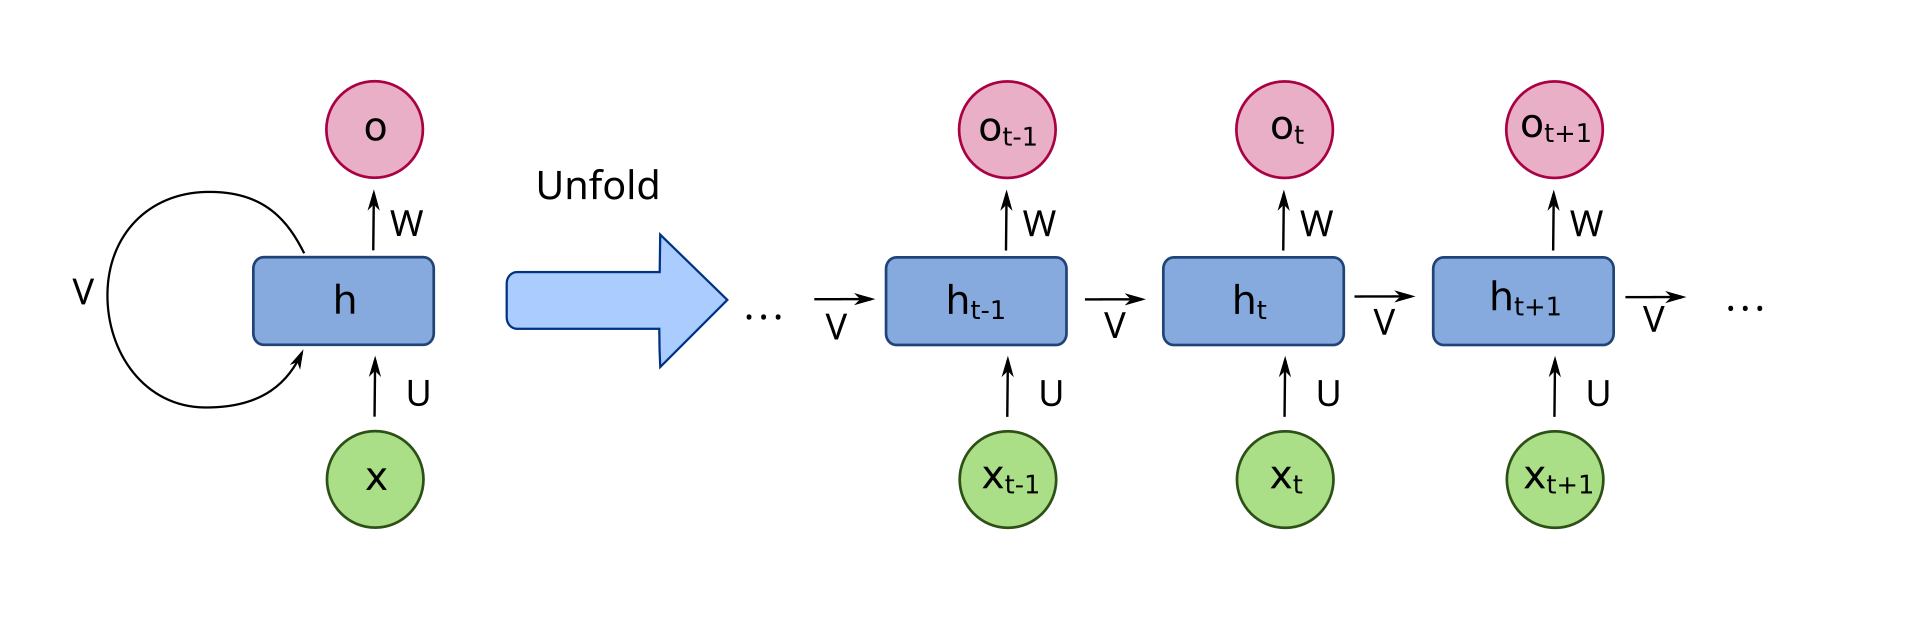
\includegraphics[width=0.8\textwidth]{images/SOTA/rnn.png}
    \caption{Rete Neurale Ricorrente e \textit{unfolding}. Fonte: \url{https://commons.wikimedia.org/w/index.php?curid=60109157} }
\end{figure}
Nonostante la capacità teorica delle RNN di processare sequenze di lunghezza arbitraria, la loro applicazione pratica è limitata a causa di una serie di problematiche molto note. Come dimostrato matematicamente da Bengio et al. \cite{bengio1994learning}, l'addestramento di questi modelli è ostacolato dal fenomeno della scomparsa o dell'esplosione del gradiente. Questa criticità rende estremamente difficile per il modello correlare informazioni distanti all'interno della sequenza temporale. Al fine di contrastare questi fenomeni nascono le reti \textbf{Long Short Term Memory} (LSTM) \cite{lstm} e \textbf{Gated Recurrent Units} (GRU) \cite{DBLP:journals/corr/ChoMGBSB14}, che introducono il concetto di \textit{gating} per contrastare le problematiche legate al gradiente. Per anni questa tipologia di modelli ha costituito lo stato dell'arte per i dati sequenziali, nonostante delle limitazioni note, ad esempio la necessità di elaborare i dati in modo sequenziale (parola per parola nel caso di elaborazione del linguaggio naturale) rendendo impossibile la parallelizzazione del calcolo tramite hardware moderno (GPU), oppure la difficoltà con le dipendenze a lungo termine all'interno delle sequenze.
\section{I modelli Transformer}
I modelli \textit{Transformer} trovano le loro origini nel meccanismo di
\textbf{Attenzione}, nato anni prima nell'ambito dei modelli
\textit{encoder-decoder}, in particolare con le reti \textit{seq2seq}
\cite{seq2seq}, utilizzate nell'ambito della traduzione automatica. In questa
tipologia di modelli il \textit{decoder}, tipicamente costituito da una RNN,
utilizza un unico vettore, lo stato finale dell'\textit{encoder} (anche in
questo caso si trattava solitamente di una RNN), che riassume la sequenza di
input per poi generare l'output.
\begin{figure}[H]
    \centering
    \includegraphics[width=0.7\textwidth]{images/SOTA/seq2seq.png}
    \caption{Inferenza con modelli \textit{seq2seq}. Fonte: \url{https://github.com/d2l-ai/d2l-en} }
\end{figure}
La grande limitazione di questi modelli risiede proprio nell'utilizzo di un singolo vettore statico per la fase di decodifica, che non risulta sufficiente a riassumere adeguatamente la sequenza in input. Inoltre, se quest'ultima risulta particolarmente lunga, dato l'utilizzo di modelli RNN o LSTM, le informazioni legate ai primi dati in ingresso potevano essere perdute a causa della grande distanza dallo stato finale. Allo scopo di superare i limiti del vettore di contesto e migliorare quindi le prestazioni dei modelli \textit{seq2seq} viene introdotto per la prima volta un meccanismo di attenzione da Bahdanau et al. \cite{bahdanau2016neuralmachinetranslationjointly}.
\begin{figure}[H]
    \centering
    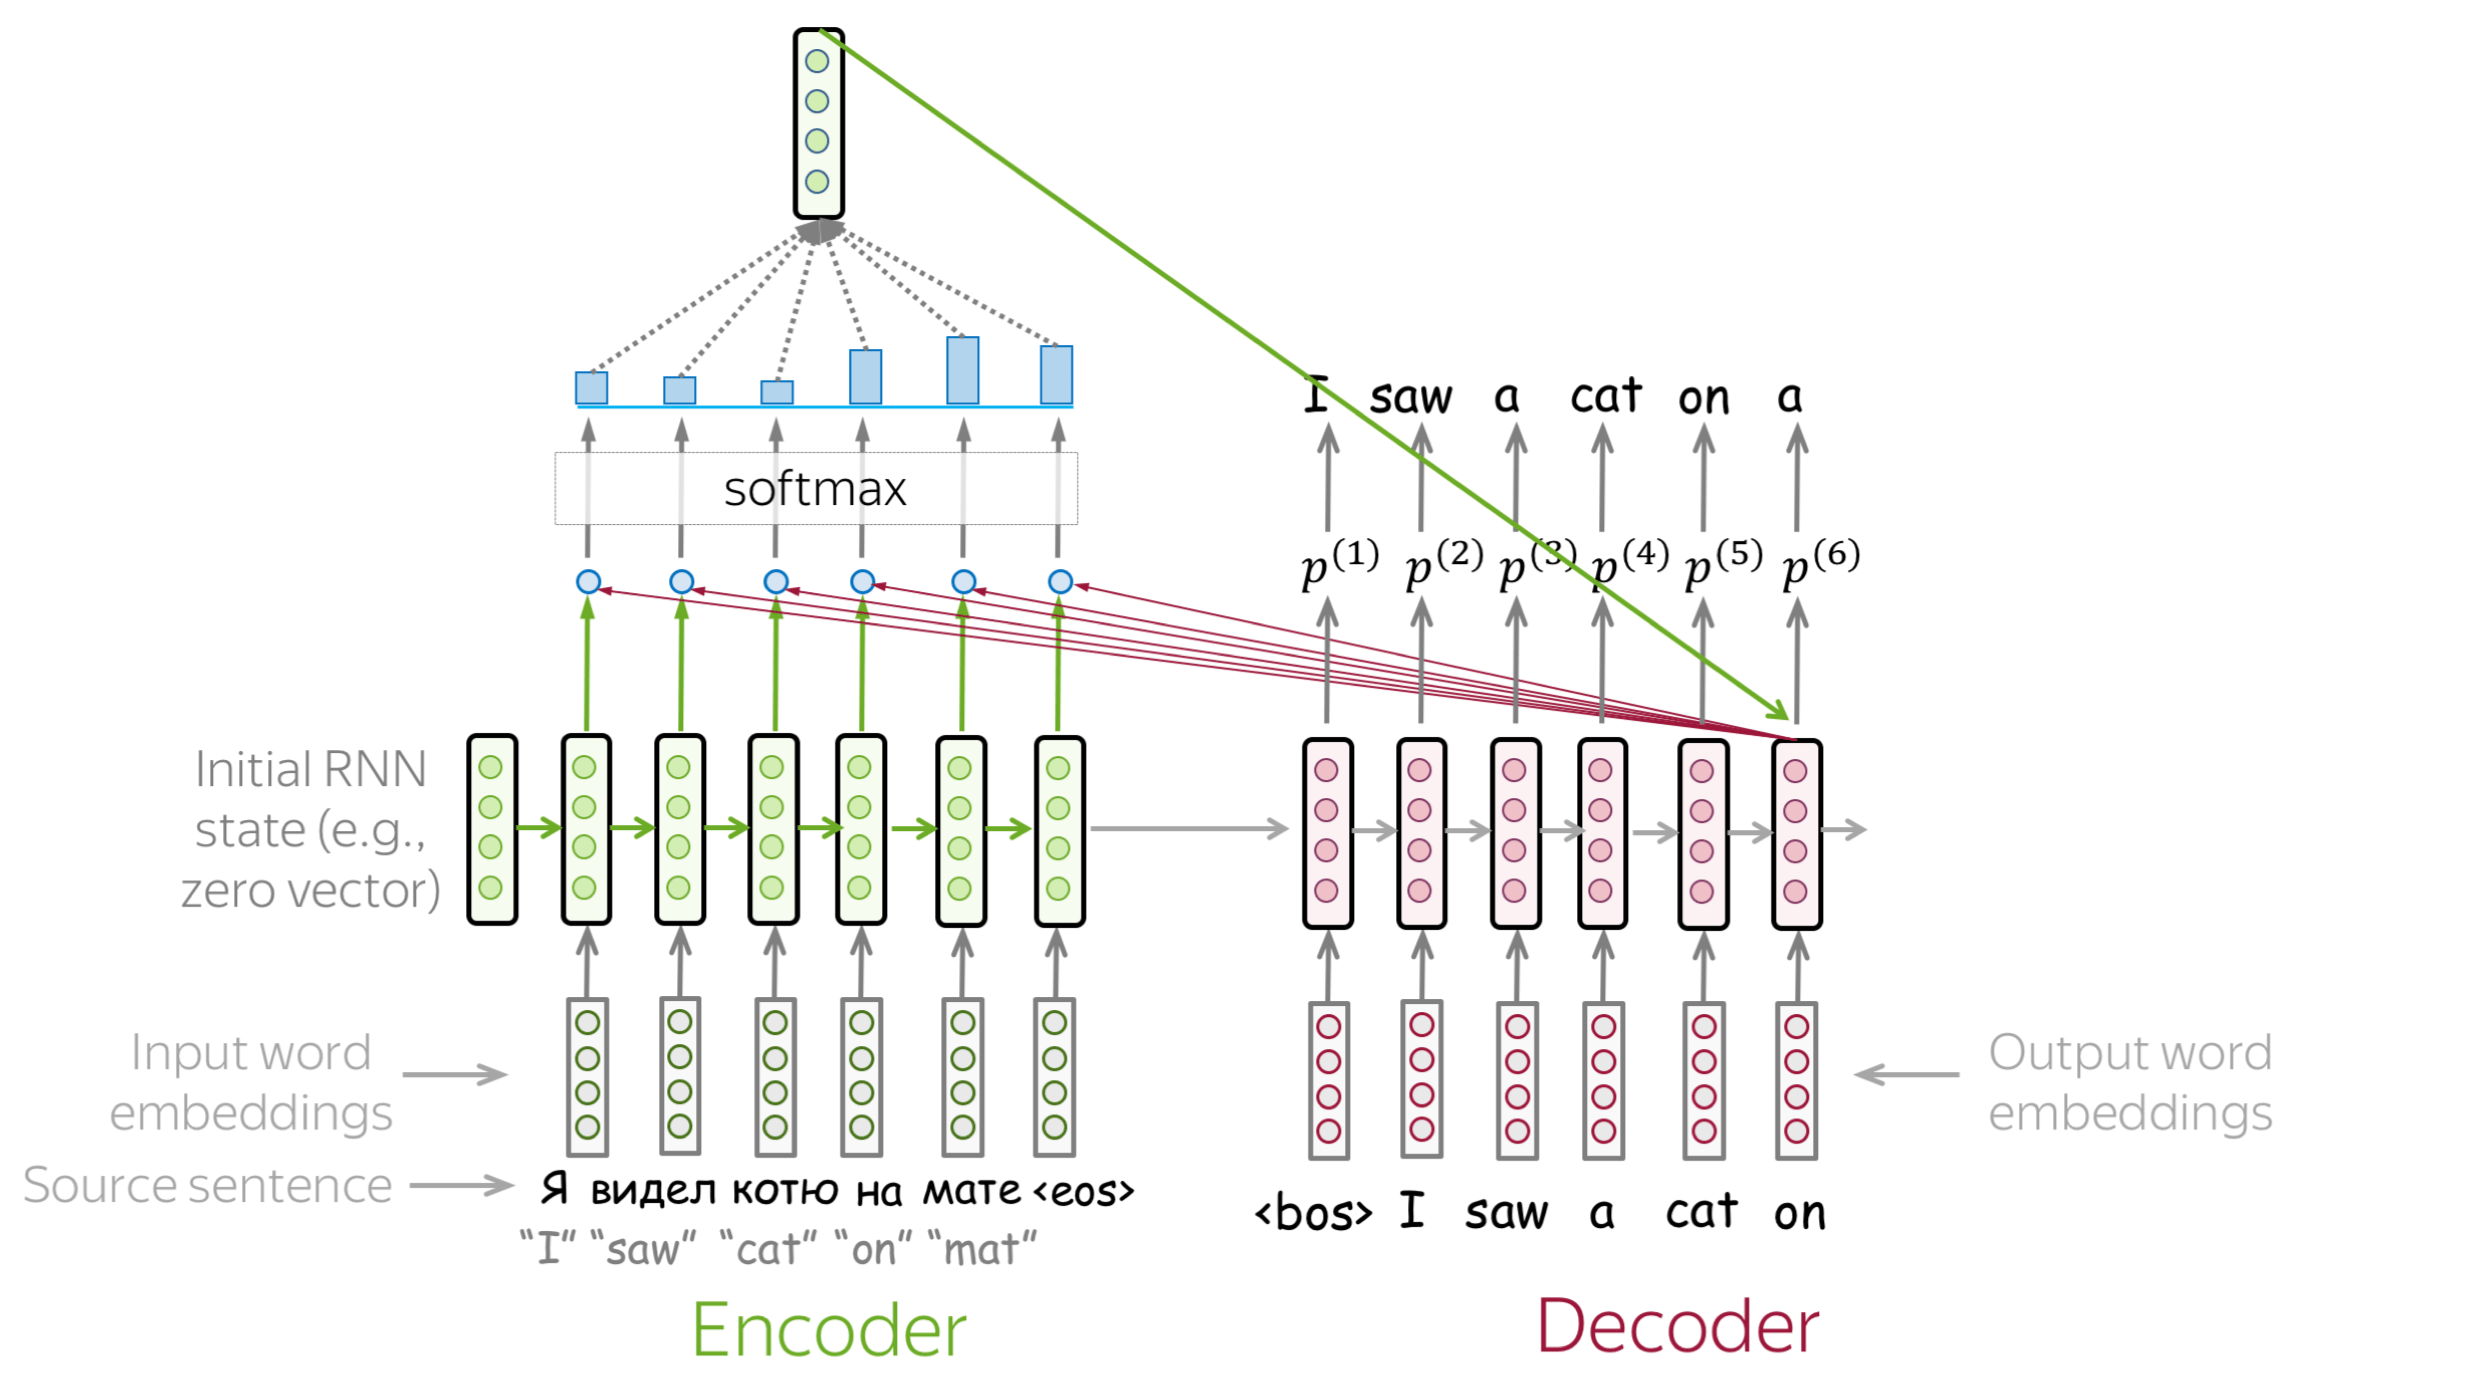
\includegraphics[width=1.0\textwidth]{images/SOTA/attn.png}
    \caption{Meccanismo di attenzione nei modelli \textit{seq2seq}. Fonte: \url{https://lena-voita.github.io/nlp_course/seq2seq_and_attention.html} }
\end{figure}
Questo meccanismo rende dinamico il vettore di contesto, che viene calcolato per ogni iterazione di decodifica pesando i contributi di tutti gli stati intermedi ottenuti dall'\textit{encoder}. In questo modo è possibile fornire in input al modello \textit{decoder} un vettore che riassume adeguatamente la sequenza in ingresso, dando maggiore importanza alle porzioni realmente rilevanti per l'output e migliorando nettamente le prestazioni dei modelli \textit{seq2seq}. \par
Nonostante l'introduzione dell'attenzione abbia rappresentato una svolta nel
superamento del limite costituito dal vettore di contesto statico, queste
architetture rimanevano ancora profondamente legate alla natura sequenziale
delle RNN o LSTM. In tale configurazione, l'attenzione agisce solo come un
meccanismo ausiliario tra l'\textit{encoder} e il \textit{decoder}, e
l'elaborazione dei dati avviene un passo alla volta, impedendo qualsiasi tipo
di parallelizzazione dei calcoli. \par
La vera rivoluzione si verifica con l'introduzione dell'architettura
\textbf{Transformer} \cite{AttentionIsAllYouNeed}, che abbandona interamente
l'approccio sequenziale delle reti ricorrenti per passare a quello delle reti
\textit{feed-forward}, utilizzando la \textbf{Multi-Head Self Attention}. In
particolare, l'architettura proposta da Vaswani et al. è di tipo
\textit{encoder-decoder}, poiché è stata utilizzata e testata sul dominio della
traduzione automatica.
\begin{figure}[H]
    \centering
    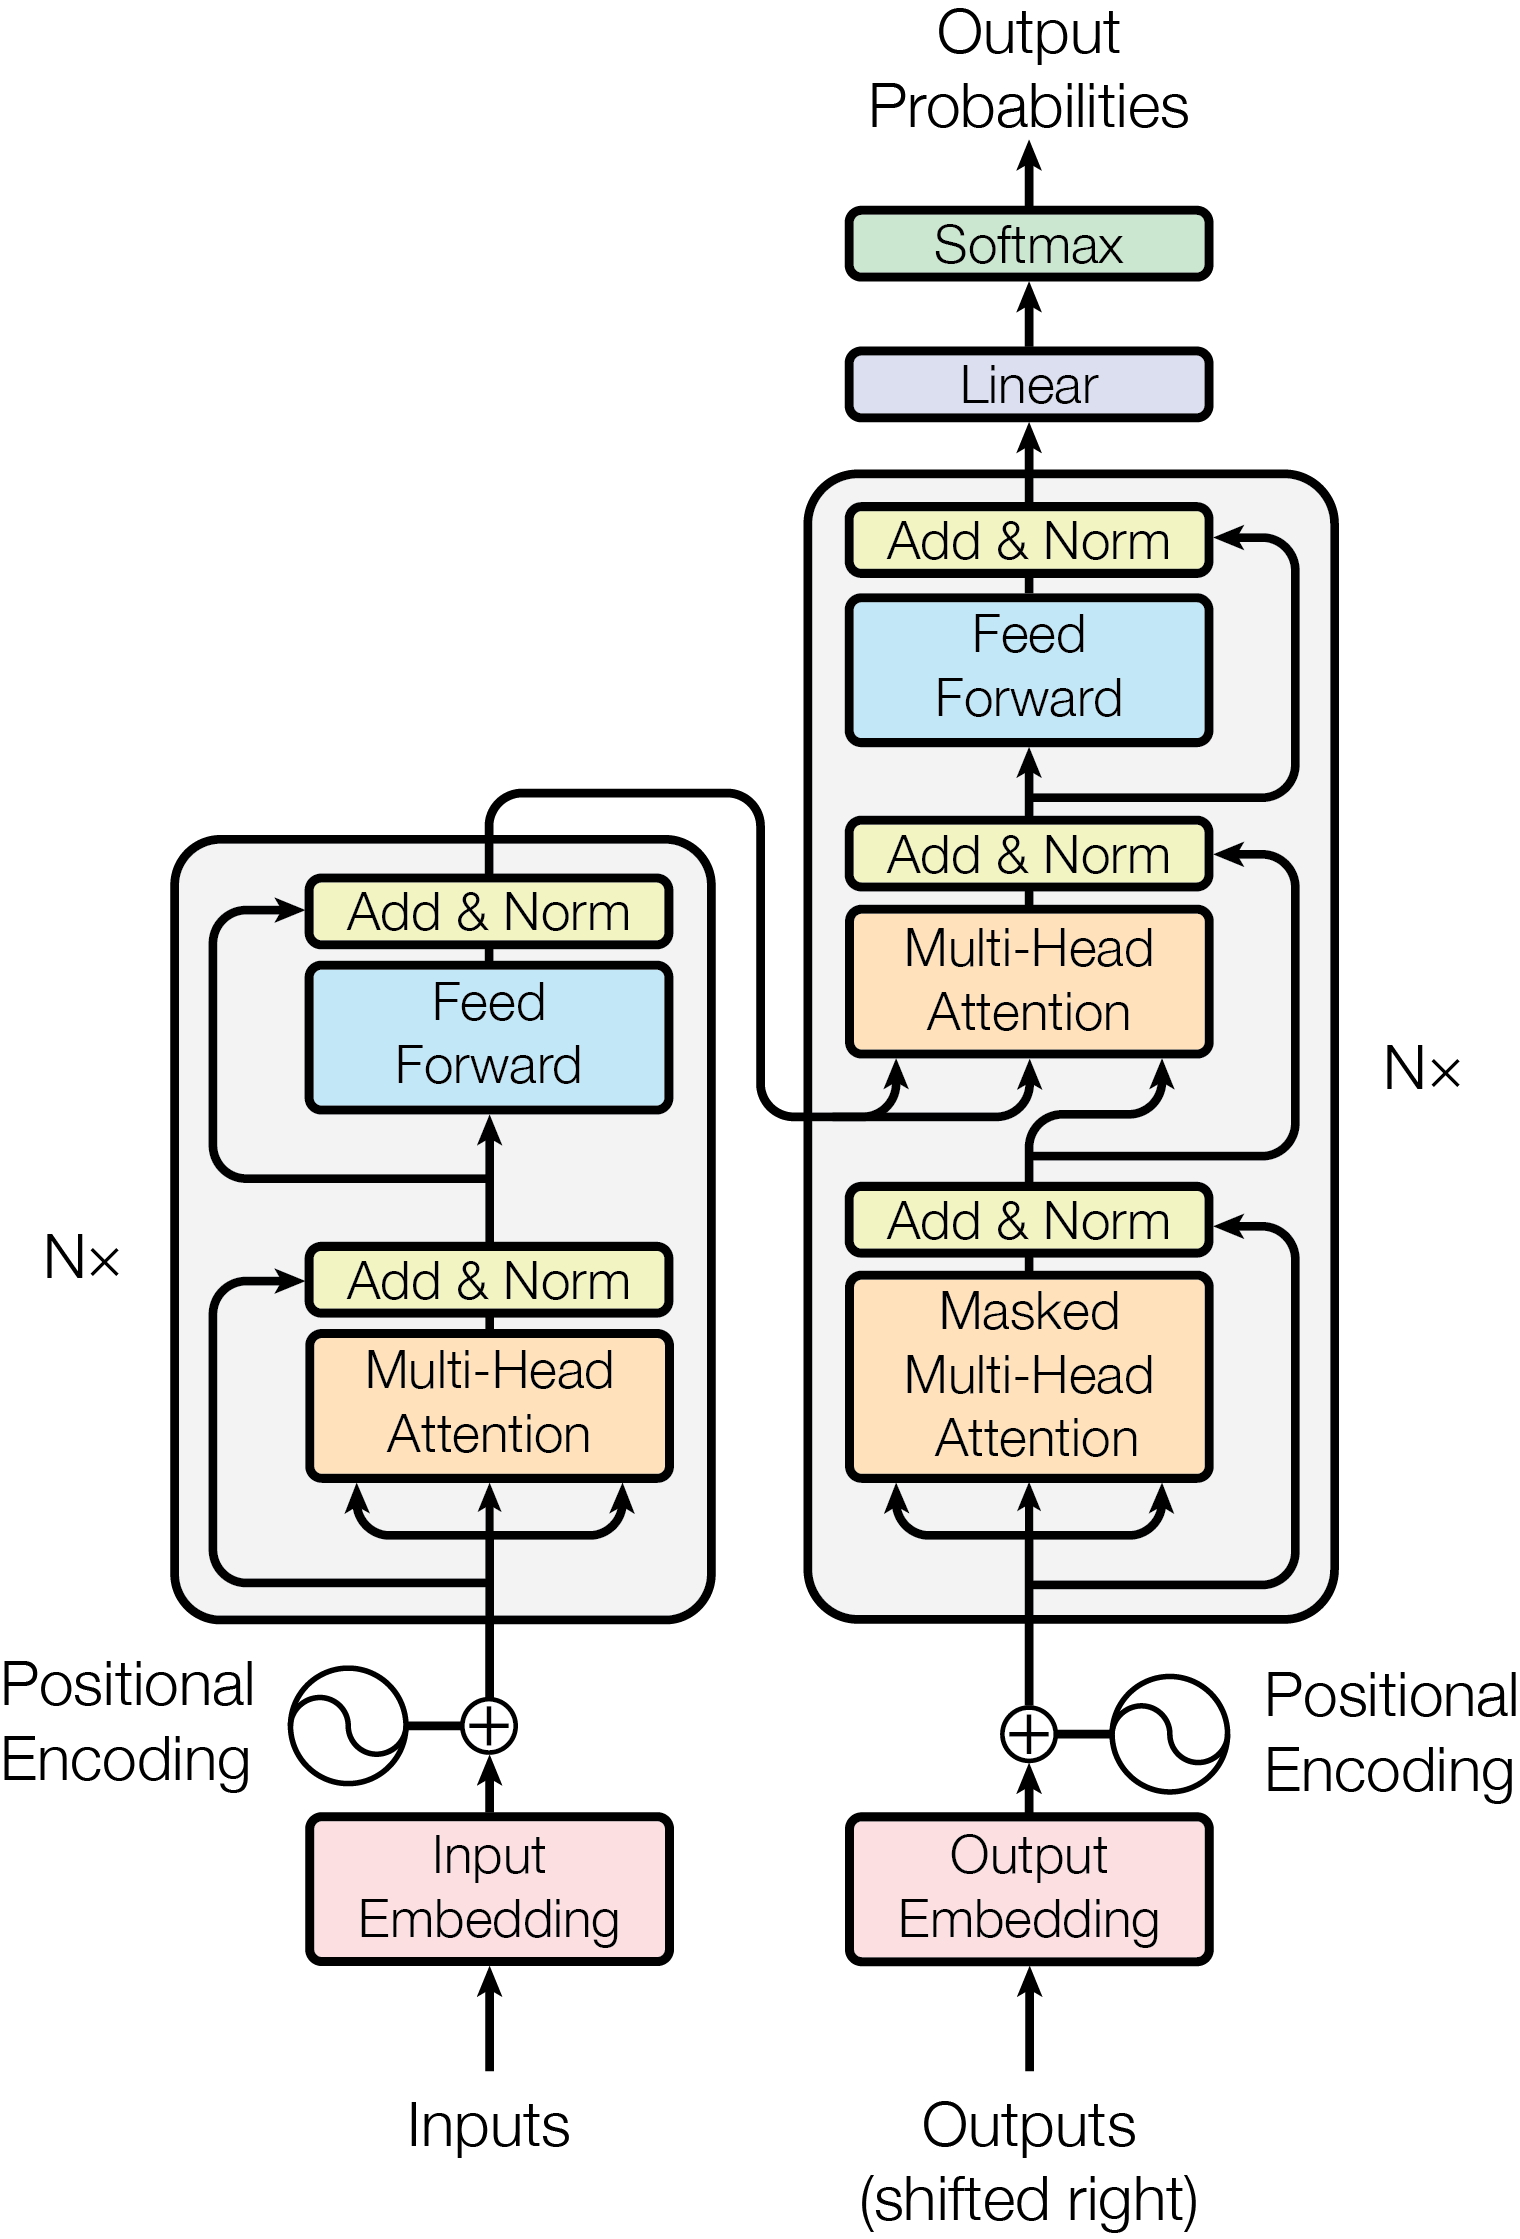
\includegraphics[width=0.5\textwidth]{images/SOTA/Transformer.png}
    \caption{Architettura Transformer originaria proposta da Vaswani et al. Fonte: \cite{AttentionIsAllYouNeed} }
    \label{figure:attn_is_all_you_need}
\end{figure}
Questa architettura si compone di una serie di blocchi, i cosiddetti blocchi \textit{Transformer}, posti in cascata attraverso un flusso residuale (al fine di evitare i fenomeni della scomparsa dei gradienti) e formati da tra componenti principali:
\begin{itemize}
    \item \textbf{Multi-Head Self Attention (MHSA):} rappresenta il cuore del blocco, permette al modello di proiettare l'input in diversi spazi di rappresentazione e catturare relazioni globali tra gli elementi della sequenza.

    \item \textbf{Layer Normalization (LayerNorm):} introdotta da Ba et al. \cite{ba2016layernormalization}, viene applicata prima (o dopo, a seconda della variante \textit{Pre-Norm} o \textit{Post-Norm} \cite{xiong2020layernormalizationtransformerarchitecture}) di ogni blocco funzionale, stabilizza le attivazioni e accelera la convergenza dell'addestramento, garantendo che la distribuzione dei dati rimanga consistente attraverso i vari layer.

    \item \textbf{Feed-Forward Network (FFN):} tipicamente costituita da due trasformazioni lineari intervallate da una funzione di attivazione non lineare (come la \textit{GELU} \cite{hendrycks2023gaussianerrorlinearunits} o la \textit{ReLU} \cite{agarap2019deeplearningusingrectified}). Questo modulo, spesso chiamato \textbf{MLP} (\textit{Multi-Layer Perceptron}), opera in modo indipendente su ogni posizione della sequenza, permettendo di elaborare e ricombinare le informazioni estratte dal meccanismo di attenzione.
\end{itemize}
Notare che l'architettura Transformer non possiede meccanismi intrinseci per gestire l'ordine sequenziale dei dati (a differenza delle RNN), di conseguenza è necessario introdurre il \textbf{Positional Encoding}(\cite{shaw2018selfattentionrelativepositionrepresentations}\cite{su2023roformerenhancedtransformerrotary}). Si tratta di vettori che vengono sommati ai vettori di input per fornire al modello informazioni sulla posizione relativa o assoluta di ogni elemento nella sequenza.
Il nodo cruciale di questa architettura è il meccanismo di \textbf{Self Attention}, che risulta strutturalmente differente da quanto introdotto da Bahdanau et al. \cite{bahdanau2016neuralmachinetranslationjointly}, poiché non si tratta più di un calcolo di similarità tra lo stato corrente del \textit{decoder} (output) e gli stati intermedi dell'\textit{encoder} (input). In questo nuovo meccanismo sono i singoli elementi della sequenza in input che interagiscono tra di loro, permettendo di catturare le dipendenze contestuali indipendentemente dalla distanza fra gli elementi coinvolti. In particolare, la \textit{Self Attention}, detto $x$ un elemento della sequenza in input $X = {x_1, x_2,\dots, x_n}$, esegue tre proiezioni lineari che producono le \textit{query}, le \textit{key} e i \textit{value}
\begin{equation}
    \begin{aligned}
        q & = W_q x \\
        k & = W_k x \\
        v & = W_v x
    \end{aligned}
\end{equation}
Considerato l'i-esimo elemento della sequenza $x_i$, viene calcolato il prodotto scalare tra la \textit{query} corrispondente $q_i$ e le \textit{key} di tutti gli altri elementi della sequenza. Il risultato esprime il grado di affinità o "attenzione" che l'elemento i-esimo deve porre verso gli altri elementi. Questi punteggi vengono poi normalizzati ad una distribuzione di probabilità tramite una funzione \textit{softmax}.
\begin{equation}
    \alpha_{ij} = \text{softmax} \left( \frac{q_i \cdot k_j}{\sqrt{d_k}} \right) = \frac{\exp \left( \frac{q_i \cdot k_j}{\sqrt{d_k}} \right)}{\sum_{l=1}^{n} \exp \left( \frac{q_i \cdot k_l}{\sqrt{d_k}} \right)}
\end{equation}
Infine, viene eseguita una somma pesata dei vettori \textit{value} $v$ per ottenere l'uscita del meccanismo di attenzione.
\begin{equation}
    a_i = \sum_{j=1}^{n} \alpha_{ij} v_j
\end{equation}
Tuttavia, il vero punto di forza dell'architettura Transformer risiede nella capacità di parallelizzare questa operazione attraverso la \textbf{Scaled-Dot-Product Attention}.
\begin{figure}[H]
    \centering
    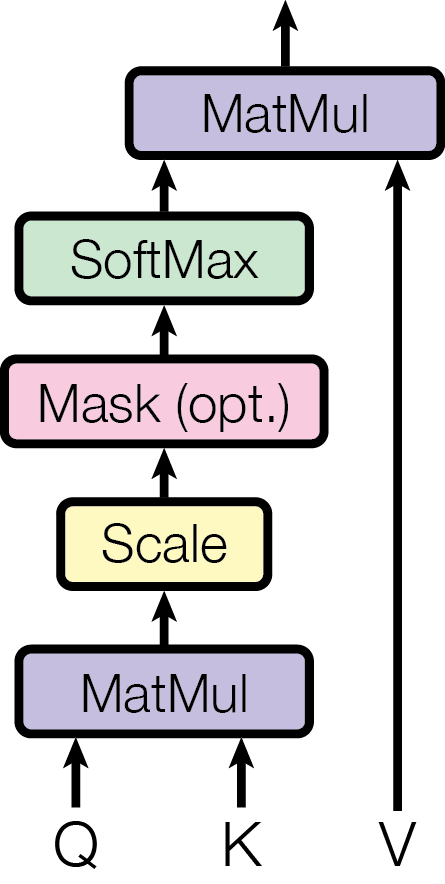
\includegraphics[width=0.2\textwidth]{images/SOTA/mhsa_detail.png}
    \caption{Visualizzazione dell'operazione di \textit{Scaled-Dot-Product Attention}. Fonte: \cite{AttentionIsAllYouNeed} }
    \label{figure:attn_mask}
\end{figure}
Invece di calcolare l'attenzione un elemento alla volta, le proiezioni di tutti gli $n$ elementi della sequenza vengono raggruppate in matrici $Q, K, V \in \mathbb{R}^{n \times d}$, permettendo di eseguire l'intero calcolo tramite il prodotto matriciale, facilmente parallelizzabile tramite hardware apposito (GPU oppure TPU).
\begin{equation}
    \text{Attention}(Q, K, V) = \text{softmax} \left( \frac{QK^T}{\sqrt{d_k}} \right) V
\end{equation}
Questa formulazione evidenzia i costi computazionali dell'architettura: il prodotto $QK^T$ genera una matrice di attenzione di dimensione $n \times n$, portando a una complessità quadratica $O(n^2)$ (temporale e spaziale) rispetto alla lunghezza della sequenza. Di conseguenza, il vantaggio rispetto alle architetture RNN, dato dalla possibilità di parallelizzare e velocizzare le operazioni sull'intera sequenza, comporta un aumento del costo computazionale (le RNN hanno costo lineare $O(n)$). \par
Al fine di aumentare la capacità di questa nuova architettura viene introdotto
il concetto di \textbf{Multi-Head Attention}, attraverso il quale è possibile
dotare il meccanismo di attenzione di molteplici "teste" che operano estraendo
\textit{features} e rappresentazioni differenti dalla sequenza in input. Quanto
descritto in precedenza viene applicato all'interno di ogni \textit{attention
    head} e successivamente gli output vengono concatenati e proiettati in uno
spazio della dimensione originale della rappresentazione.
\begin{figure}[H]
    \centering
    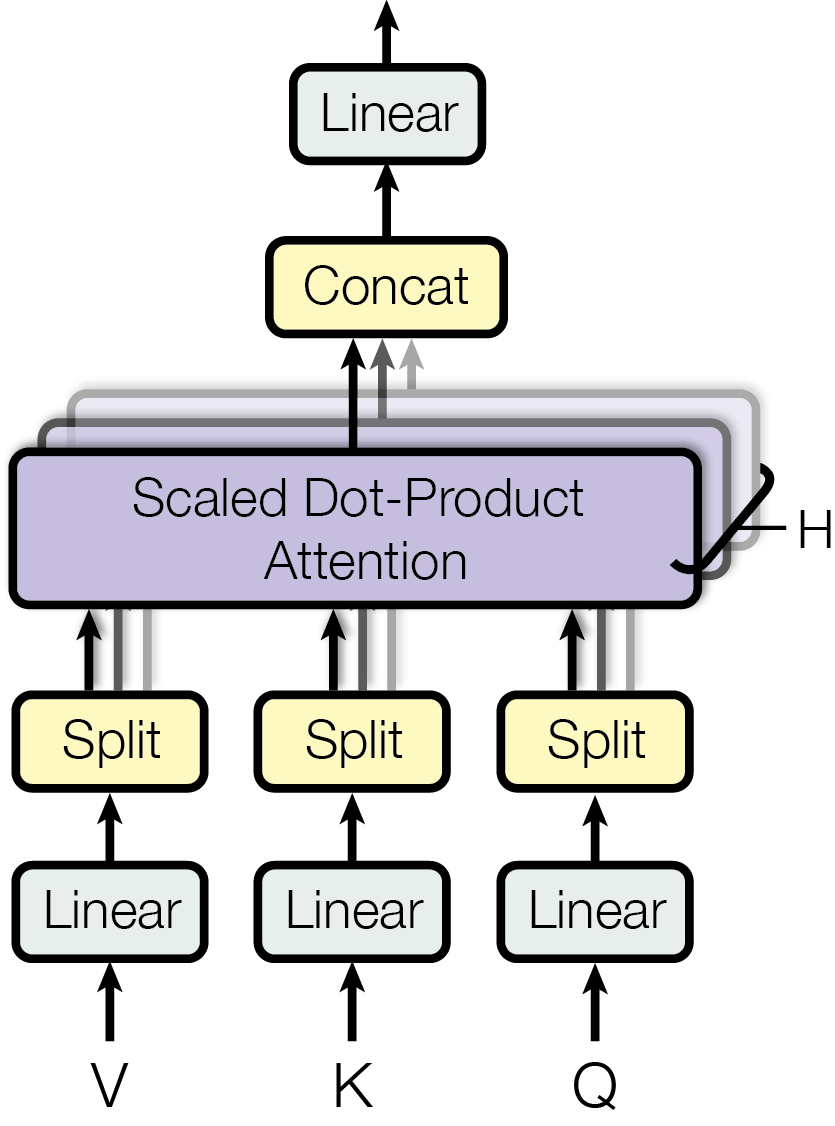
\includegraphics[width=0.35\textwidth]{images/SOTA/MHSA.png}
    \caption{\textit{Multi Head Self Attention}. Fonte: \cite{AttentionIsAllYouNeed} }
\end{figure}

Per concludere la trattazione dei modelli \textit{transformer} è necessario affrontare
l'utilizzo della \textbf{mascheratura} (\textit{masking}). Come è possibile
notare dalla Figura \ref{figure:attn_is_all_you_need}, vi sono due tipologie di
blocchi \textit{Transfomer}: i blocchi \textit{encoder} e i blocchi
\textit{decoder}. Nei primi, ogni elemento può interagire con ogni altro
elemento della sequenza (attenzione bi-direzionale), permettendo di estrarre
una rappresentazione contestuale completa di contesto destro e sinistro. Al
contrario, nei secondi (usati nei modelli generativi di linguaggio), viene
applicata una maschera durante la fase di attenzione (Figura
\ref{figure:attn_mask}). Tale maschera pone a $-\infty$ i valori della matrice
di attenzione relativi agli elementi successivi nella sequenza, garantendo che,
attraverso la funzione \textit{softmax}, i pesi di attenzione corrispondenti
vengano azzerati. In questo modo la predizione (della parola successiva, nel
caso dei modelli generativi del linguaggio) dipenderà esclusivamente dai
termini che la precedono (contesto sinistro), preservando così la causalità
necessaria durante l'inferenza.
\section{Vision Transformer}
Per quanto concerne l'ambito della visione artificiale, per anni le \textbf{Reti Neurali Convoluzionali} (CNN) hanno dominato il campo grazie alla loro capacità di estrarre le \textit{features} spaziali delle immagini attraverso l'uso di filtri appresi che vengono applicati alle immagini. Il successo delle CNN è dovuto principalmente a due proprietà intrinseche: l'\textbf{invarianza alla traslazione} e la \textbf{località dei dati}. Grazie ai filtri convoluzionali, queste reti sono in grado di riconoscere pattern indipendentemente dalla loro posizione nell'immagine e di elaborare le relazioni tra pixel vicini in modo estremamente efficiente. Tuttavia, questo approccio presenta un limite fondamentale: la natura locale delle convoluzioni rende difficile catturare le \textbf{relazioni a lungo raggio} tra pixel distanti, se non attraverso l'utilizzo di numerosi strati, posti in cascata, che aumentano progressivamente il campo ricettivo (\textit{receptive field}) \cite{luo2017understandingeffectivereceptivefield}. \par
\begin{figure}[H]
    \centering
    \includegraphics[width=0.8\textwidth]{images/SOTA/ViT_original.pdf}
    \caption{Architettura del Vision Transformer (ViT). Fonte: \cite{dosovitskiy2021imageworth16x16words} }
\end{figure}
L'introduzione dei modelli \textit{Transformer} ha portato alla nascita dei \textbf{Vision Transformer} (ViT) \cite{dosovitskiy2021imageworth16x16words}, che utilizzano un'architettura \textit{Encoder-Only} per applicare il meccanismo di attenzione all'ambito della visione artificiale. In particolare, l'architettura ViT suddivide l'immagine in regioni, dette \textit{patch}, non sovrapposte (ad esempio, \textit{patch} di dimensione $16 \times 16$ pixel), che vengono poi appiattiti e proiettati in uno spazio di rappresentazione tramite una trasformazione lineare. Questi vettori di rappresentazione delle patch vengono quindi arricchiti con informazioni posizionali e forniti ad una serie di blocchi \textit{Transformer-Encoder} simili a quelli descritti in precedenza. \par
\begin{figure}[H]
    \centering
    
\includegraphics[width=0.8\textwidth]{images/MHSA.png}
    \caption{Struttura della \textit{Multi Head Attention}.}
\end{figure}
\begin{figure}[H]
    \centering
    \includegraphics[width=0.8\textwidth]{images/MLP.png}
    \caption{Struttura del \textit{Multi Layer Perceptron} nei blocchi Transformer del ViT.}
\end{figure}
Sfruttando il meccanismo di attenzione, i ViT permettono alle regioni dell'immagine di interagire tra loro, catturando relazioni a lungo raggio molto più facilmente rispetto alle CNN. Nonostante i ViT abbiano dimostrato prestazioni competitive rispetto alle CNN, soprattutto su dataset di grandi dimensioni, presentano ancora alcune limitazioni, come la necessità di grandi quantità di dati per l'addestramento \cite{steiner2022trainvitdataaugmentation} e la complessità computazionale elevata, dovuta alla natura quadratica del meccanismo di attenzione. Tuttavia, l'utilizzo di questi modelli sta crescendo rapidamente (soprattutto come \textit{backbone} o \textit{Vision Encoder} all'interno di architetture modulari \cite{kirillov2023segment}\cite{radford2021learningtransferablevisualmodels}), portando a numerose varianti e miglioramenti che cercano di mitigare queste criticità, come l'introduzione di meccanismi di attenzione più efficienti o l'adozione di approcci ibridi che combinano le CNN con i ViT. \par
\begin{figure}[H]
    \centering
    \includegraphics[width=0.4\textwidth]{images/SOTA/DeiT.pdf}
    \caption{Architettura del Data-efficient Image Transformer (DeiT). Fonte: \cite{touvron2021trainingdataefficientimagetransformers}}
\end{figure}
Una delle prime varianti che hanno migliorato il ViT originale è stata il \textbf{Data-efficient Image Transformer} (DeiT) \cite{touvron2021trainingdataefficientimagetransformers}, che ha introdotto un nuovo metodo di addestramento chiamato \textit{knowledge distillation}, in cui un modello ("student") viene addestrato a imitare le predizioni di un modello pre-addestrato ("teacher"), ottenendo prestazioni competitive anche con dataset di dimensioni ridotte. Questa tecnica, applicata ad uno speciale \textit{token} di distillazione, ha permesso al DeiT di raggiungere risultati paragonabili a quelli del ViT originale, ma con un minor quantitativo di dati.
\begin{figure}[H]
    \centering
    \includegraphics[width=1.0\textwidth]{images/SOTA/SWIN_arch.pdf}
    \caption{Architettura di \textit{Swin Transformer}. Fonte: \cite{liu2021swintransformerhierarchicalvision}}
\end{figure}
Successivamente, è stato proposto lo \textbf{Swin Transformer} \cite{liu2021swintransformerhierarchicalvision}, che introduce meccanismi di attenzione gerarchici e a finestre mobili per migliorare l'efficienza computazionale. A differenza del ViT che mantiene una risoluzione costante, lo \textit{Swin Transformer} riduce gradualmente la risoluzione spaziale man mano che si scende in profondità nella rete, unendo le patch vicine (Patch Merging). Questo crea una struttura gerarchica simile a quella delle reti neurali convoluzionali (CNN), permettendo al modello di vedere sia dettagli piccoli che strutture grandi. Inoltre, invece di calcolare l'attenzione su tutta l'immagine, lo \textit{Swin Transformer} la calcola all'interno di finestre locali di \textit{patch} non sovrapposte, introducendo meccanismi di località simili a quelli delle CNN.
\begin{figure}[H]
    \centering
    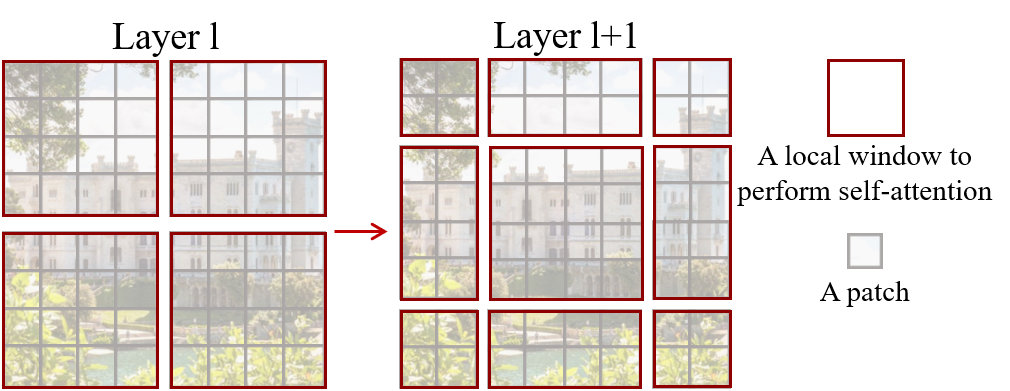
\includegraphics[width=0.7\textwidth]{images/SOTA/SWIN_window.png}
    \caption{Meccaniscmo di Shifted Window. Fonte: \cite{liu2021swintransformerhierarchicalvision}}
\end{figure}
Allo stesso tempo viene introdotto un meccanismo di \textit{Shifted Window} che permette alle finestre di patch di interagire tra loro nel blocco successivo, garantendo che le informazioni vengano propagate attraverso l'intera immagine. Grazie a queste innovazioni, lo \textit{Swin Transformer} è in grado di raggiungere prestazioni all'avanguardia su una varietà di compiti di visione artificiale, come la classificazione delle immagini, il rilevamento degli oggetti e la segmentazione semantica, con un'efficienza computazionale significativamente migliorata rispetto al ViT originale. \par

\chapter{Stato dell'arte}
Data la rapida evoluzione nel campo della visione artificiale, l'analisi dello
stato dell'arte risulta fondamentale per identificare le metodologie più
promettenti volte a coniugare elevate prestazioni e sostenibilità
computazionale. In questo capitolo verrà esaminato il panorama delle soluzioni
atte a rendere i \textbf{Vision Transformer} (ViT) applicabili in scenari
reali, caratterizzati da vincoli di latenza, memoria e consumo energetico.
Notare che nessuna soluzione esclude automaticamente le altre, spesso molti di
questi approcci vengono integrati e combinati per ottenere risultati migliori.
\begin{figure}[H]
    \centering
    \includegraphics[width=0.75\textwidth]{images/SOTA/tassonomia.pdf}
    \caption{Tassonomia delle principali metodologie per l'efficientamento dei modelli di visione artificiale.}
\end{figure}
La trattazione si articolerà su due fronti principali:
\begin{itemize}
    \item \textbf{Ottimizzazione Architetturale:} l'analisi di modelli e architetture appositamente progettate per ridurre la complessità computazionale, i costi di memoria o anche i consumi energetici dell'inferenza.
          \begin{itemize}
              \item \textbf{Architetture Ibride:} si tratta di architetture che integrano elementi tipici dei modelli \textit{Transformer} con elementi tipici delle reti convoluzionali, al fine di sfruttare i punti di forza di entrambe le tipologie di modelli e ottenere un buon compromesso tra prestazioni e efficienza;
              \item \textbf{Architetture Edge-Optimized}: modelli progettati specificamente per essere eseguiti su dispositivi con risorse limitate, come smartphone o dispositivi IoT, con l'obiettivo di massimizzare le prestazioni mantenendo un basso consumo energetico e ridotti requisiti computazionali.
              \item \textbf{Neural Architecture Search (NAS):} ovvero l'automazione del processo di design di architetture ottimali in termini di costi e prestazioni.
          \end{itemize}
    \item \textbf{Tecniche di Compressione dei modelli:} lo studio di metodologie applicabili a reti pre-esistenti al fine di ridurne la dimensione e migliorarne l'efficienza, tra cui:
          \begin{itemize}
              \item \textbf{Pruning:} ovvero la rimozione di pesi, teste di attenzione o interi blocchi ridondanti dall'architettura per snellire il modello senza compromettere significativamente le prestazioni;
              \item \textbf{Quantizzazione:} cioé la riduzione della precisione numerica della rappresentazione dei parametri, ottenendo modelli molto più compatti in termini di memoria e veloci da eseguire su hardware specializzato;
              \item \textbf{Knowledge Distillation:} il trasferimento di conoscenza da modelli \textit{teacher} grandi e complessi a modelli \textit{student} più piccoli e leggeri, aumentando in modo importante le prestazioni ottenibili da questi ultimi;

          \end{itemize}
\end{itemize}
\section{Architetture efficienti di ViT}
\subsection{Architetture Ibride}
A partire dall'introduzione dei \textit{Vision Transformer} (ViT) da parte di
Dosovitskiy et al.\cite{dosovitskiy2021imageworth16x16words}, numerosi sforzi
sono stati fatti per sviluppare architetture che potessero mantenere le
prestazioni elevate dei ViT, ma con una complessità computazionale ridotta. Tra
queste, le architetture ibride rappresentano una delle direzioni più
promettenti ed esplorate.
\subsubsection{BoTNet}
Uno dei primi approcci è stato quello presentato da Srinivas et
al.\cite{srinivas2021bottlenecktransformersvisualrecognition}, nel quale è
stata modificata una architettura ResNet \cite{he2015deepresiduallearningimage}
sostituendo le convoluzioni spaziali $(3x3)$ negli ultimi 3 blocchi (definiti
\textit{bottleneck}) con delle Multi-Head Self-Attention.
\begin{figure}[H]
    \centering
    \includegraphics[width=0.6\textwidth]{images/SOTA/BoTNet.pdf}
    \caption{Confronto tra il blocco ResNet e il blocco BoTNet. Fonte: \cite{srinivas2021bottlenecktransformersvisualrecognition}.}
\end{figure}
In particolare questa architettura ha dimostrato delle performance migliori rispetto alla ResNet-50, con un numero di parametri simile, ma con una complessità computazionale più elevata, data dall'introduzione dell'attenzione. Questo lavoro ha dimostrato che l'integrazione delle due architetture è una direzione di ricerca promettente, ma è necessario trovare un compromesso tra prestazioni e complessità computazionale.
\subsubsection{CvT}
I pionieri dell'applicazione delle convoluzioni ad un ViT sono stati Wu et.
al\cite{wu2021cvtintroducingconvolutionsvision}, con il loro
\textbf{Convolutional Vision Transformer}, che ha introdotto delle convoluzioni
per produrre le query, key e value all'interno di nuovi \textit{Convolutional
    Transformer Block}, integrando profondamente le due architetture. Questo tipo
di approccio ha eliminato la necessità del \textit{Positional Encoding} tramite
le proprietà delle convoluzioni.
\begin{figure}[H]
    \centering
    \includegraphics[width=0.8\textwidth]{images/SOTA/cvt.pdf}
    \caption{A sinistra l'architettura CvT, a destra la struttura del blocco \textit{Convolutional Transformer}. Fonte: \cite{wu2021cvtintroducingconvolutionsvision}.}
\end{figure}
Questo tipo di soluzione ha permesso di raggiungere ottime performance su vari task, mantenendo contenuto il numero di parametri.
\subsubsection{CoAtNet}
Un ulteriore pilastro di questo approccio ibrido è quello di Dai et
al.\cite{dai2021coatnetmarryingconvolutionattention}, i quali hanno proposto
un'architettura CNN-\textit{Transformer} definita \textbf{Co-AtNet}, con
l'obiettivo di sfruttare i punti di forza delle due architetture. In
particolare, gli autori hanno combinato blocchi convoluzionali
\textit{Depthwise} e moduli di \textit{Self-Attention} organizzandoli in stadi
successivi, con l'obiettivo di ridurre la complessità computazionale mantenendo
elevate prestazioni.
\begin{figure}[H]
    \centering
    \includegraphics[width=0.85\textwidth]{images/SOTA/coatnet_arch.pdf}
    \caption{L'architettura di CoAtNet.Fonte: \cite{dai2021coatnetmarryingconvolutionattention}.}
\end{figure}
Gli autori hanno dimostrato che questo approccio permette di raggiungere prestazioni superiori rispetto a molte architetture CNN e ViT, con un numero di parametri e un numero di operazioni in virgola mobile inferiori.
\subsubsection{FastViT}
Di recente, ulteriori sviluppi sono stati presentati da Vasu et al.
\cite{vasu2023fastvitfasthybridvision} con l'architettura \textbf{FastViT},
nella quale si affronta il problema della latenza causata dai frequenti accessi
in memoria necessari durante l'inferenza. In particolare, le connessioni
residuali, seppur fondamentali per evitare la scomparsa del gradiente,
contribuiscono pesantemente a questo problema, richiedendo di recuperare
continuamente dalla memoria i valori sui quali eseguire la somma.
\begin{figure}[H]
    \centering
    \includegraphics[width=0.9\textwidth]{images/SOTA/fastvit_arch.pdf}
    \caption{L'architettura del modello FastViT. Fonte: \cite{vasu2023fastvitfasthybridvision}.}
\end{figure}
Gli autori risolvono questo problema applicando una \textbf{riparametrizzazione strutturale post-addestramento} all'interno di un modulo proprietario denominato \textbf{RepMixer}. Durante il \textit{training}, la rete sfrutta connessioni residuali e convoluzioni su rami paralleli per massimizzare la capacità di apprendimento; in fase di inferenza, queste strutture parallele vengono fuse matematicamente in un'unica convoluzione di tipo \textit{depthwise}. Questo approccio permette di eliminare del tutto le operazioni di somma e i relativi accessi in memoria, mantenendo inalterate le elevate prestazioni predittive.
Infine, sebbene l'architettura di \textit{FastViT} affidi i primi tre stadi interamente a operazioni convoluzionali per abbattere rapidamente la risoluzione, nell'ultimo stadio viene introdotta la \textit{Self-Attention}. Questa scelta strategica permette di ampliare il \textit{receptive-field} e catturare le dipendenze globali solo quando la mappa delle \textit{feature} è sufficientemente ridotta, evitando un aumento eccessivo della complessità computazionale. Grazie a queste soluzioni, il modello raggiunge prestazioni uguali o superiori alle architetture ibride di riferimento, ma con latenza e operazioni in virgola mobile (FLOPs) drasticamente inferiori.
\subsubsection{FasterViT}
Una ulteriore direzione di ricerca è quella di modificare il meccanismo di
attenzione, al fine di introdurlo in una architettura basata su CNN, per
limitare i costi introdotti. In questo senso Hatamizadeh et al.
\cite{hatamizadeh2024fastervitfastvisiontransformers} propongono l'architettura
\textbf{FasterViT}, nella quale viene introdotto un nuovo meccanismo di
attenzione, denominato \textbf{Hierarchical Attention}.
\begin{figure}[H]
    \centering
    \includegraphics[width=0.95\textwidth]{images/SOTA/fastervit_arch_horizontal.pdf}
    \caption{L'architettura del modello FasterViT. Fonte: \cite{hatamizadeh2024fastervitfastvisiontransformers}.}
\end{figure}
L'approccio proposto risulta particolarmente efficace nei casi in cui vengono elaborati input ad alta risoluzione, in queste situazioni il calcolo della \textit{Self-Attention} globale diventa rapidamente proibitivo a causa del suo costo computazionale quadratico. D'altra parte, limitare l'attenzione a finestre spaziali isolate (come avviene nello \textit{Swin Transformer}) comporta la perdita cruciale del contesto globale. Per superare questo ostacolo, gli autori propongono una macro-architettura ibrida strutturata in quattro stadi sequenziali. I primi due stadi operano esclusivamente tramite blocchi residui convoluzionali, i quali estraggono le \textit{feature} locali ed eseguono un sottocampionamento spaziale. Soltanto nel terzo e quarto stadio, dove la risoluzione delle \textit{feature map} risulta notevolmente ridotta, intervengono i moduli \textit{Transformer}.
\begin{figure}[H]
    \centering
    \includegraphics[width=0.2\textwidth]{images/SOTA/fastervit_HAT.pdf}
    \caption{Mappa di attenzione del meccanismo di \textit{Hierarchical Attention}. Fonte: \cite{hatamizadeh2024fastervitfastvisiontransformers}.}
\end{figure}
La vera innovazione di \textit{FasterViT} risiede nel nuovo meccanismo di \textbf{Hierarchical Attention (HAT)} utilizzato in questi ultimi stadi. Il modello introduce dei \textit{Carrier Tokens} (token portatori) che agiscono come ponte informativo: questi speciali \textit{token} riassumono prima le informazioni all'interno delle singole finestre locali, interagiscono poi tra di loro a livello globale scambiandosi il contesto generale dell'immagine e, infine, ritrasmettono l'informazione globale aggiornata ai \textit{token} delle rispettive finestre locali. Questo approccio si avvicina ad un concetto di un \textit{receptive-field} globale ma con una frazione del costo computazionale originale. Utilizzando queste novità \textit{FasterViT} riesce a stabilire nuovi standard di velocità ed efficienza, dimostrando che l'uso sinergico di convoluzioni iniziali e attenzione negli ultimi stadi è una strategia molto efficace per ottenere ottime prestazioni con costi computazionali contenuti.
\subsubsection{Vision Mamba}
Infine, negli ultimissimi anni, il concetto di ibridazione si è spinto oltre la
combinazione di CNN e \textit{Transformer} classici. Per far fronte alla
necessità di elaborare sequenze visive o immagini ad altissima risoluzione con
complessità strettamente lineare $\mathcal{O}(N)$, la ricerca più recente ha
iniziato a sostituire i moduli di attenzione globale con i Modelli a Spazio di
Stato (SSM), in particolare la loro declinazione denominata \textbf{Mamba}
\cite{gu2024mambalineartimesequencemodeling}.
\begin{figure}[H]
    \centering
    \includegraphics[width=0.9\textwidth]{images/SOTA/vision_mamba.pdf}
    \caption{Architettura di Vision Mamba. Fonte: \cite{zhu2024visionmambaefficientvisual}.}
\end{figure}
Architetture ibride emergenti, come le varianti convoluzionali di \textbf{Vision Mamba (Vim)} \cite{zhu2024visionmambaefficientvisual}, integrano l'estrazione di \textit{feature} locali tipica delle CNN con il ragionamento sequenziale bidirezionale degli SSM. Sebbene i ViT ibridi rimangano lo standard di fatto nell'industria odierna, questa nuova frontiera CNN-SSM rappresenta la naturale evoluzione per abbattere definitivamente il costo quadratico dell'attenzione.
\subsection{Architetture Edge-Optimized}
Uno dei principali ostacoli all'implementazione dei ViT in scenari reali è
rappresentato dalle grandi difficoltà nell'esecuzione su dispositivi con
risorse limitate, come smartphone o dispositivi IoT. Per affrontare questo
problema sono stati fatti dei grandi passi avanti sia in ambito hardware,
implementando acceleratori specializzati per l'esecuzione di modelli neurali
(NPU, \textit{Neural Processing Unit}), sia in ambito architetturale,
progettando modelli specificamente ottimizzati per i dispositivi \textit{edge}.
\subsubsection{MobileViT}
Uno dei primi lavori in questo senso è stato quello di Mehta et al.
\cite{mehta2022mobilevitlightweightgeneralpurposemobilefriendly}, con il famoso
\textbf{MobileViT} che utilizza un approccio ibrido per coniugare l'efficienza
computazionale delle CNN con la capacità di catturare dipendenze globali dei
ViT.
\begin{figure}[H]
    \centering
    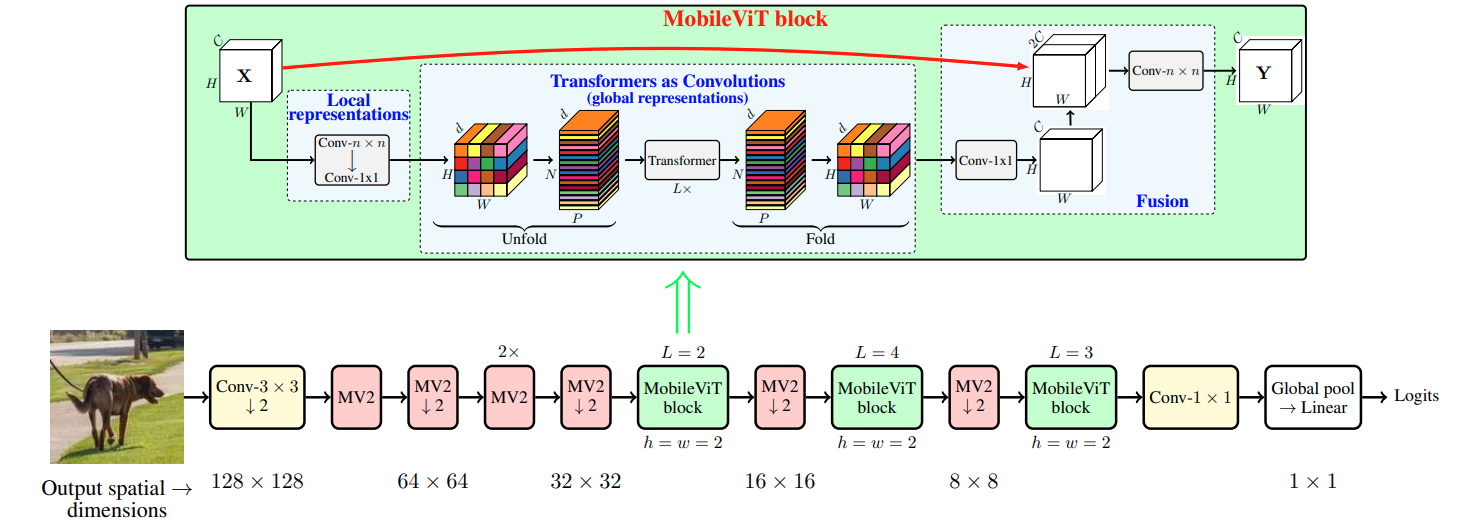
\includegraphics[width=0.95\textwidth]{images/SOTA/mobilevit_arch.png}
    \caption{Architettura di MobileViT. Fonte: \cite{mehta2022mobilevitlightweightgeneralpurposemobilefriendly}.}
\end{figure}
Scendendo in profondità, l'architettura di MobileViT è composta principalmente da blocchi MV2 (MobileNetV2 \cite{sandler2019mobilenetv2invertedresidualslinear}), che si occupano di eseguire il sottocampionamento e catturare le dipendenze locali, alternati da blocchi \textit{MobileViT}. Questi ultimi costituiscono il contributo più significativo di questo lavoro. A differenza dei classici \textit{Vision Transformer} che appiattiscono irrimediabilmente le singole \textit{patch} rovinando la topologia bidimensionale dell'immagine, i blocchi \textit{MobileViT} preservano la geometria spaziale elaborando le dipendenze globali in modo mirato.
\begin{figure}[H]
    \centering
    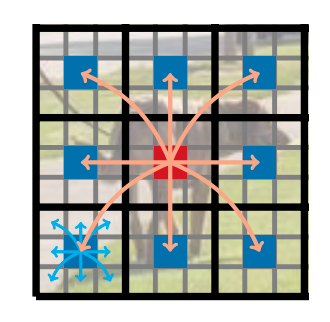
\includegraphics[width=0.3\textwidth]{images/SOTA/mobilevit_attn.png}
    \caption{Meccanismo di attenzione di MobileViT. Fonte: \cite{mehta2022mobilevitlightweightgeneralpurposemobilefriendly}.}
\end{figure}
Per ottenere questo risultato, il blocco esegue un'operazione matematica che
gli autori definiscono \textit{unfolding} (srotolamento). La mappa delle
\textit{feature} viene idealmente divisa in piccole finestre, o \textit{patch}.
Per costruire le sequenze monodimensionali rigorosamente richieste dal
\textit{Transformer}, il modello non fonde i pixel della singola
\textit{patch}, ma estrae esclusivamente i pixel che occupano la stessa posizione spaziale all'interno di tutte le \textit{patch}
dell'immagine (ad esempio, raggruppando tutti i pixel in alto a sinistra di
ogni finestra). Ognuno di questi pixel estratti rappresenta un singolo
\textit{token}. L'insieme di questi pixel omologhi forma la sequenza su cui viene calcolata la
\textit{Self-Attention}. Questo approccio si rivela vincente perché permette di
ottenere un campo recettivo globale a livello di singolo pixel senza pagarne il
reale prezzo computazionale. Infatti, calcolare un'attenzione globale su tutti
i pixel dell'immagine contemporaneamente comporterebbe un costo elevatissimo, insostenibile per un dispositivo mobile; calcolandola invece in parallelo su
queste specifiche sotto-sequenze posizionali, il costo totale viene abbattuto
drasticamente. Terminato il calcolo dell'attenzione, entra in gioco
l'operazione inversa, definita \textit{folding} (ripiegamento). I pixel appena
aggiornati dal \textit{Transformer} vengono ricollocati nelle
loro coordinate 2D di origine, restituendo in uscita una mappa spaziale intatta
e pronta per le elaborazioni successive.
Tramite questo approccio, MobileViT raggiunge e supera le prestazioni sia delle CNN, che dei ViT tradizionali, risultando più efficiente di questi ultimi ma non delle prime.
\subsubsection{Mobile-Former}
In \cite{chen2022mobileformerbridgingmobilenettransformer}, Chen et al. propongono un'architettura innovativa che integra le due architetture \textit{MobileNet} e \textit{Transformer} in modo più profondo rispetto a MobileViT. In particolare, introducono un nuovo modulo, denominato \textbf{Mobile-Former Block}, che prevede due rami paralleli, uno convoluzionale (ispirato alla \textit{MobileNet}) e uno basato su attenzione, con connessioni bidirezionali che permettono uno scambio continuo di informazioni tra i due rami.
\begin{figure}[H]
    \centering
    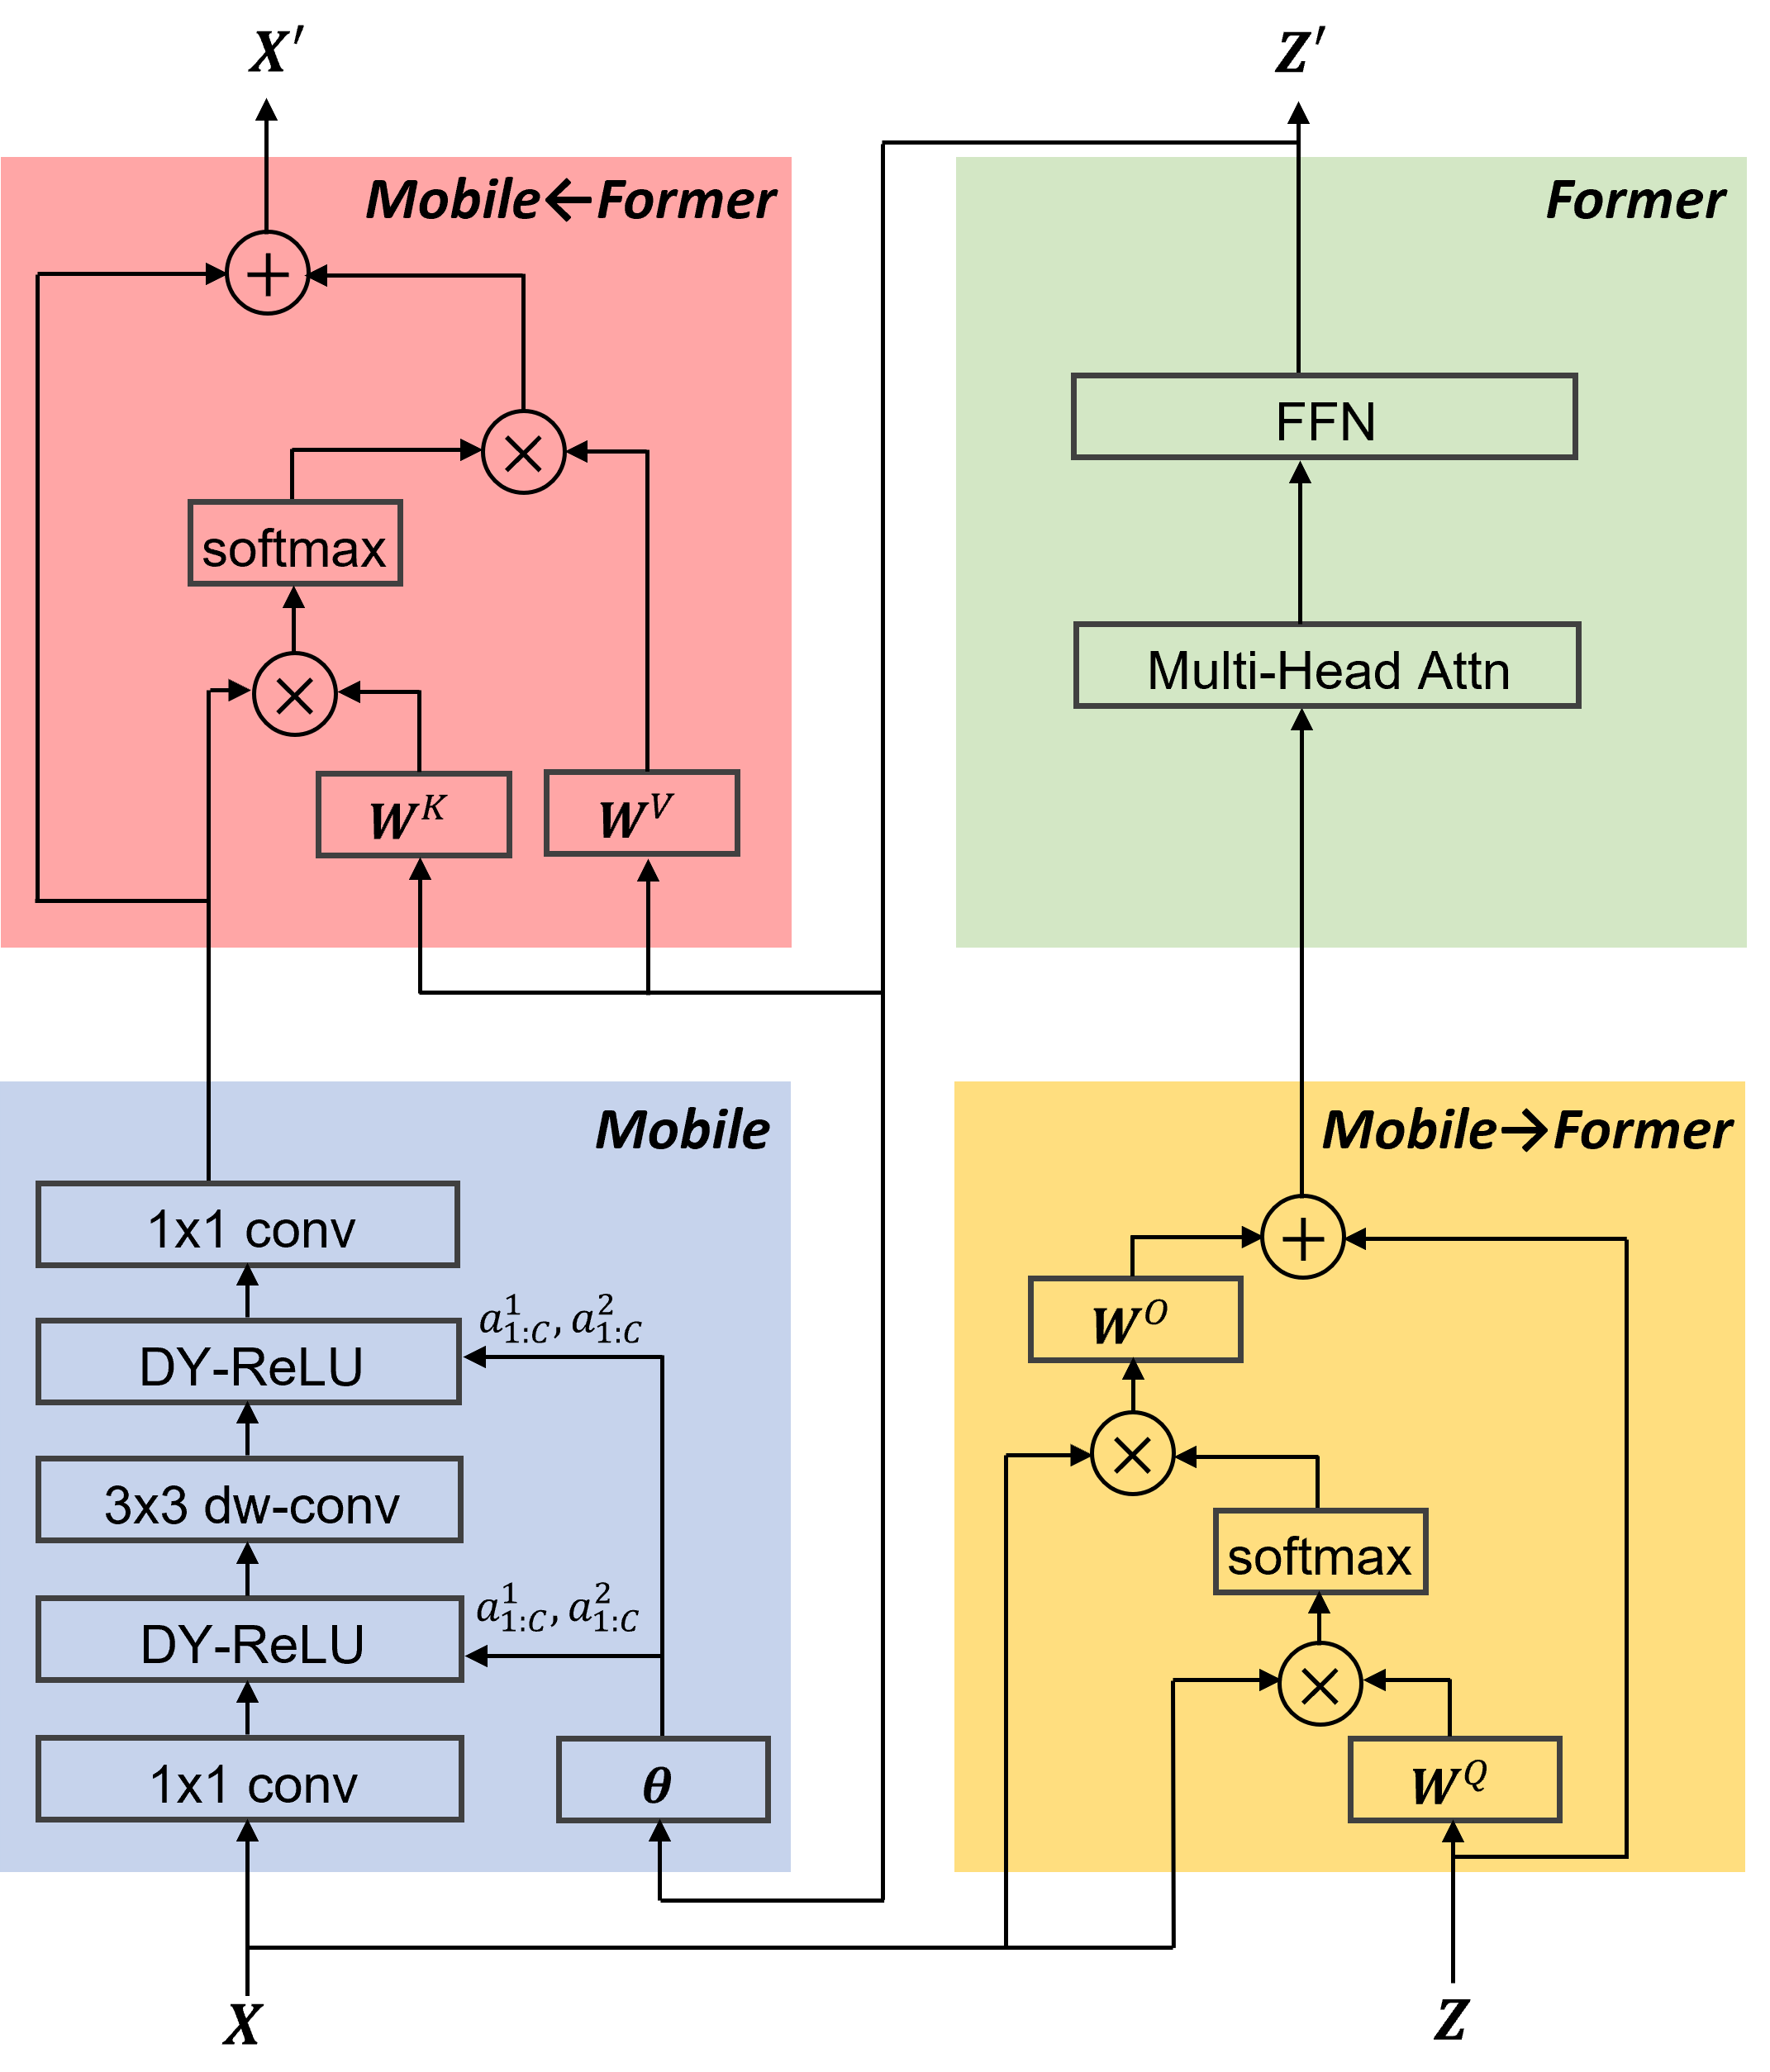
\includegraphics[width=0.36\textwidth]{images/SOTA/MobileFormerBlock.png}
    \caption{Mobile-Former Block. Fonte: \cite{chen2022mobileformerbridgingmobilenettransformer}.}
\end{figure}
Il ramo convoluzionale, che ottiene in ingresso l'intera immagine, si occupa di estrarre le \textit{features} locali, mentre il ramo basato sul meccanismo di attenzione, il quale ha in input dei token appresi, cattura le dipendenze globali. Le connessioni bidirezionali permettono a ciascun ramo di arricchire le proprie rappresentazioni con le informazioni apprese dall'altro, migliorando così la capacità complessiva del modello di comprendere sia i dettagli locali che il contesto globale dell'immagine.
Inoltre, i token utilizzati nel ramo di attenzione non sono estratti dall'immagine, come in un ViT tradizionale, ma sono appresi durante il processo di addestramento, e sono inoltre in numero molto ridotto (tipicamente 6), così da mantenere contenuto il costo computazionale dell'attenzione. Essi agiscono inizialmente da contenitori vuoti, che verranno successivamente arricchiti di informazioni provenienti dal ramo convoluzionale, e a loro volta forniranno un contesto globale che arricchirà le rappresentazioni locali di questo.
\begin{figure}[H]
    \centering
    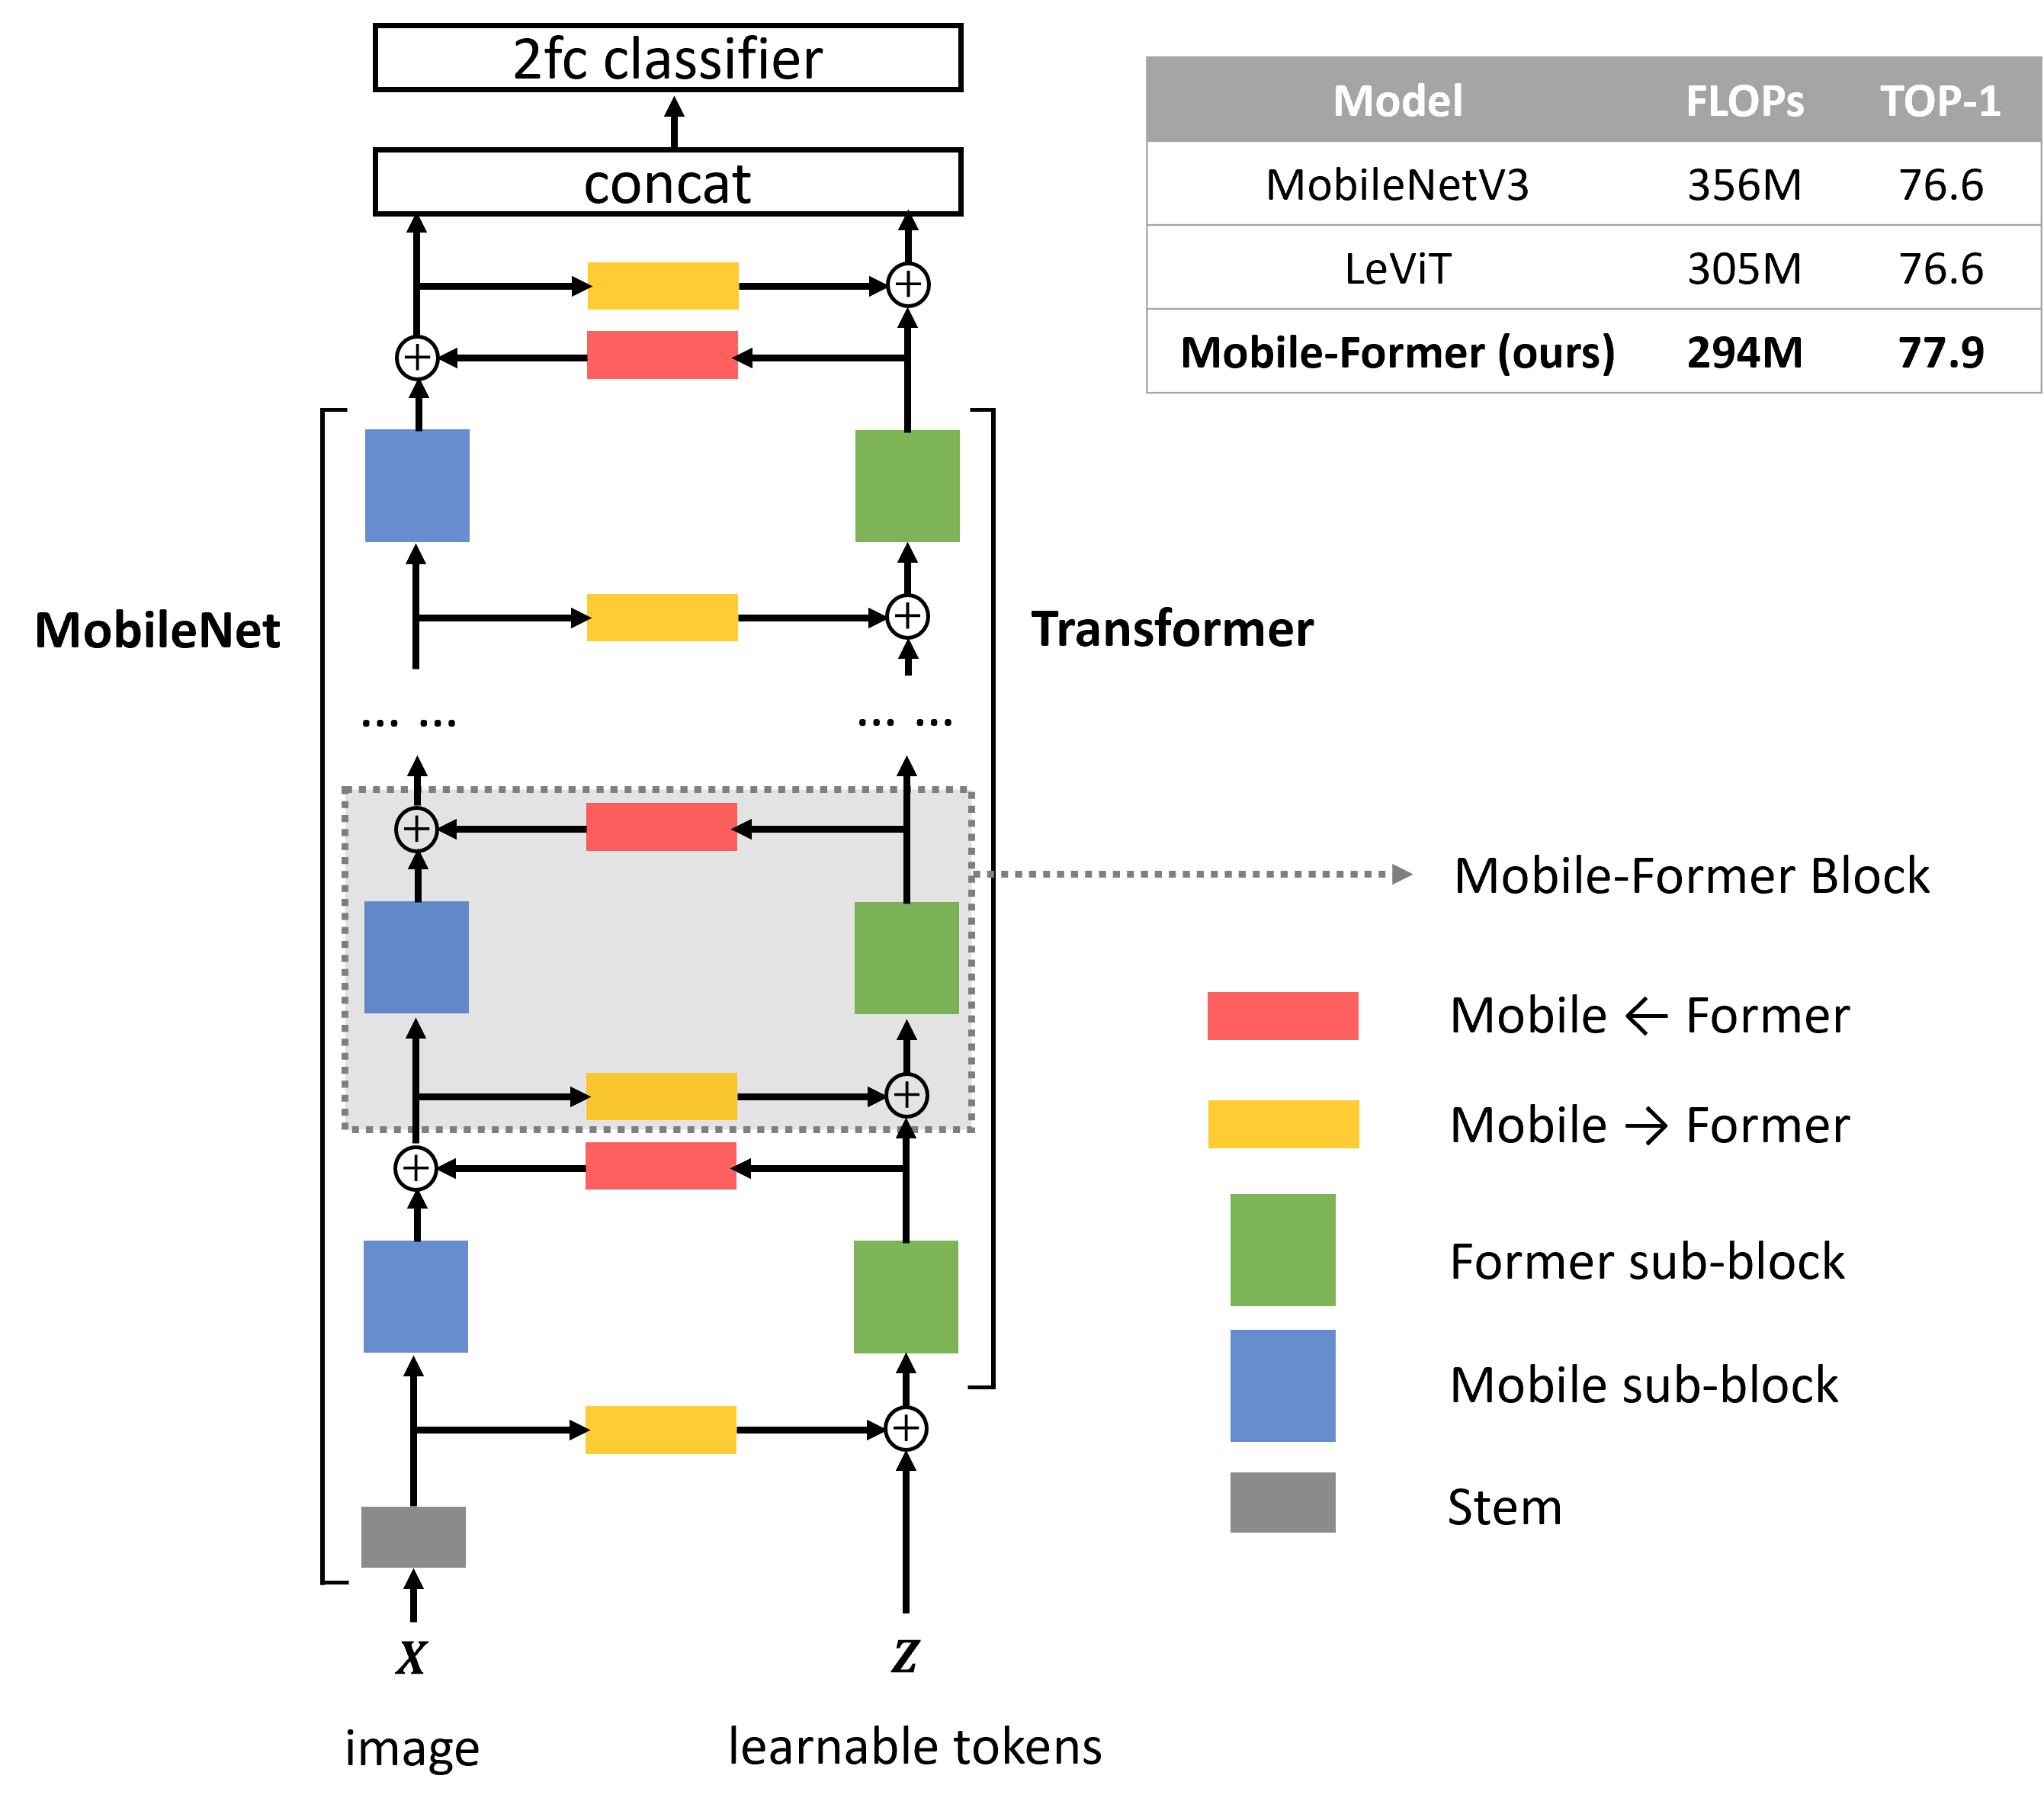
\includegraphics[width=0.6\textwidth]{images/SOTA/mobile-former.png}
    \caption{Architettura complessiva di Mobile-Former. Fonte: \cite{chen2022mobileformerbridgingmobilenettransformer}.}
\end{figure}
A valle dei blocchi \textit{Mobile-Former}, le \textit{feature map} in uscita dalla porzione convoluzionale vengono sottoposte ad una operazione di global average pooling ottenendo un vettore, a cui vengono concatenati i token del ramo di attenzione, per poi essere processati da un classificatore finale.
Grazie a questa architettura, Mobile-Former riesce a raggiungere prestazioni competitive rispetto sia ai classici modelli ViT, Swin e DeiT ma anche rispetto ad altre architetture basate su convoluzioni, con un numero di operazioni matematiche di moltiplicazione e somma (\textit{MAdds}) estremamente ridotto (circa 3-4 volte inferiori rispetto ai modelli \textit{Transformer}di riferimento), rendendolo particolarmente adatto per l'esecuzione su dispositivi mobili.
\subsubsection{EdgeViT}
Un altro esempio rilevante di architettura \textit{edge-optimized} è quello di Pan et al. \cite{pan2022edgevitscompetinglightweightcnns}, con il loro modello \textbf{EdgeViT}. Gli autori, sostenendo che \textit{MobileViT} non riesca a competere con le alternative convoluzionali ottimizzate per i dispositivi \textit{edge} in termini di compromesso tra accuratezza e complessità computazionale, propongono una nuova architettura di tipo piramidale (all'aumentare della profondità si riduce la risoluzione spaziale e aumenta il numero di canali) composta da 4 stadi che implementano un meccanismo definito \textbf{Local-Global-Local Bottleneck}, volto a ridurre il costo dell'attenzione.
\begin{figure}[H]
    \centering
    \includegraphics[width=0.75\textwidth]{images/SOTA/EdgeViT_arch.pdf}
    \caption{Architettura di EdgeViT. Fonte: \cite{pan2022edgevitscompetinglightweightcnns}.}
\end{figure}
Gli autori, partendo dal concetto di ridondanza spaziale delle immagini, che rende costosa e spesso superflua l'elaborazione di tutte le regioni dell'immagine con un meccanismo di attenzione globale, propongono una soluzione a tre fasi:
\begin{itemize}
    \item \textit{Aggregazione Locale}: per ogni token, vengono utilizzate delle convoluzioni per aggregare le informazioni provenienti da una finestra locale di dimensione fissata.
    \item \textit{Attenzione Globale Sparsa}: invece di applicare l'attenzione globale su tutti i token, vengono campionati una serie di token rappresentativi, uno per ogni finestra locale e solo su di essi viene eseguito il meccanismo di attenzione globale, riducendo drasticamente il costo computazionale.
    \item \textit{Propagazione Locale}: Vengono utilizzate delle convoluzioni trasposte per propagare le informazioni globali contenute nei token rappresentativi a tutti i token locali (all'interno della finestra). 
\end{itemize}
\begin{figure}[H]
    \centering
    \includegraphics[width=0.75\textwidth]{images/SOTA/EdgeViT_attn.pdf}
    \caption{Meccanismo di \textit{Local-Global-Local Bottleneck} applicato ad un esempio. Fonte: \cite{pan2022edgevitscompetinglightweightcnns}.}
\end{figure}
Tramite questo approccio, \textit{EdgeViT} riesce a ridurre il numero di token su cui viene calcolata l'attenzione, ma mantiene comunque la capacità di catturare dipendenze globali all'interno dell'immagine. Grazie a queste soluzioni, il modello riesce a superare le prestazioni di \textit{MobileViT} e degli altri modelli \textit{edge-optimized} e non, ottenendo un miglioramento significativo in termini di latenza. 


\subsection{Neural Architecture Search}
\section{Tecniche di compressione dei modelli}
\subsection{Quantizzazione}
\subsection{Knowledge Distillation}
\subsection{Pruning}

\chapter{Formulazione matematica del problema}
\label{cap:teoria}
Il problema in esame può essere formulato come una ricerca in uno
spazio degli stati. A partire da una architettura iniziale preaddestrata, detta
\textbf{Supernet}, si vuole identificare, tra tutte le possibili \textbf{Subnet},
quella che massimizza una determinata funzione obiettivo. In questo caso, al
fine di ottenere una compressione di modelli \textit{Transformer}, la ricerca
si configura come un problema di \textbf{ottimizzazione multi-obiettivo},
tramite il quale vengono ottimizzate sia la performance del modello (attraverso
l'accuratezza) sia la dimensione (attraverso il numero di parametri).
\newline
Una delle sfide principali che si presentano è proprio la dimensione dello
spazio degli stati, che risulta elevatissima, poiché il numero di possibili
configurazioni cresce in maniera combinatoria rispetto al numero di componenti
del modello. Nei Vision Transformer, ogni blocco Transformer presenta
molteplici gradi di libertà: è possibile variare il numero di teste di
attenzione nell'unità di \textit{Multi-Head Attention} (MHSA), la dimensione
dei vettori \textit{Query-Key} e \textit{Value}, ma anche la dimensione del
livello nascosto nel modulo \textit{Multi-Layer Perceptron} (MLP). Anche considerando un numero limitato di opzioni per ogni strato, il numero
totale di subnet candidate diventa rapidamente intrattabile per una ricerca
esaustiva. \newline Proprio per rendere trattabile l'esplorazione dello spazio
degli stati è stata scelta una formulazione conveniente del problema,
attraverso un algoritmo di ricerca \textbf{Branch and Bound} \cite{BranchAndBound} e l'utilizzo di
azioni di \textit{pruning} predefinite. L'algoritmo \textit{Branch and Bound} affronta tale complessità decomponendo ricorsivamente lo spazio di ricerca in sottoproblemi più piccoli, organizzati in una struttura ad albero (fase di \textbf{Branch}). Per ogni nodo dell'albero, viene calcolato un limite (\textbf{Bound}) del valore della funzione obiettivo: se tale limite indica che un intero ramo non può contenere una soluzione migliore di quella già individuata, il ramo viene rimosso dall'albero di ricerca. Questo meccanismo permette di navigare in modo efficiente il vasto spazio di ricerca, garantendo l'identificazione della \textit{Subnet} ottimale attraverso l'esplorazione di una frazione ridotta dello spazio degli stati complessivo.
Nella prossima sezione sarà esposta nel dettaglio la formulazione matematica proposta.\newline

\section{Formulazione della ricerca}
Dato un modello ViT $M$ con parametri $\theta$, definiamo un processo iterativo
di pruning. Per ogni iterazione viene eseguita una ricerca di tipo
\textbf{Depth First a profondità limitata}. Durante la ricerca verranno
inizialmente selezionate delle azioni da eseguire sul modello, e
successivamente, attraverso un secondo problema combinatorio vengono
selezionate le specifiche dimensioni da eliminare. L'\textbf{obiettivo} è
massimizzare la seguente funzione rispetto alla maschera binaria $m$, ai
parametri $\theta$ e al dataset $D$:
\begin{equation}
    \max_{m} \text{Obj}(m, \theta, D) = \log_2({A}(m, \theta, D)) - \lambda \cdot \log_2\left(\frac{{P}(m, \theta)}{{P}_{tot}(\theta)}\right),
\end{equation}

dove:
\begin{itemize}
    \item $m \in \{0, 1\}^N$ è la maschera di pruning globale, con $N$ numero totale di parametri del modello.
    \item La maschera è strutturata per blocchi: $m = \{m_{\mathrm{emb}}, m^{(1)}, \dots,
              m^{(i)}, \dots, m^{(L)}\}$, con $L$ numero di layer, dove $m^{(i)}$ rappresenta
          la maschera per il layer $i$-esimo, mentre $m_{\mathrm{emb}}$ rappresenta la
          maschera (globale) per la dimensione dell'embedding.
    \item Per ogni blocco $i$: $m^{(i)} = \{m_{\mathrm{head}}, m_{\mathrm{q\_k}},
              m_{\mathrm{v\_proj}}, m_{\mathrm{mlp}}\}$, con $m_{\mathrm{head}}$ la maschera
          per le teste di attenzione, $m_{\mathrm{q\_k}}$ quella per i parametri della
          proiezione query-key, $m_{\mathrm{v\_proj}}$ per la proiezione del value, e
          $m_{\mathrm{mlp}}$ per la componente \textit{Multi-Layer Perceptron} del
          blocco.
    \item ${A}(m, \theta, D)$ indica l'accuratezza del modello sul dataset $D$ con i soli parametri attivi previsti dalla maschera $m$.
    \item ${P}(m, \theta)$ rappresenta il numero di parametri attivi (non azzerati da $m$).
    \item ${P}_{tot}(\theta)$ rappresenta il numero totale di parametri del modello originale.
\end{itemize}
Notare che tramite questa formulazione è possibile ricondurre il problema in esame ad un \textbf{Problema di Programmazione Non Lineare Binario} (PNLPB) \cite{BOROS2002155}. In questo contesto, le variabili decisionali sono rappresentate dai componenti della maschera $m \in \{0, 1\}^N$, mentre la non linearità è introdotta sia dalla natura della funzione di accuratezza ${A}$ (legata ai pesi della rete neurale) sia dall'operatore logaritmico utilizzato nella funzione obiettivo. Nonostante esistano in letteratura delle tecniche di \textit{Smoothing} delle variabili binarie per risolvere questo tipo di problemi combinatori, come quelle utilizzate da Murray et al. \cite{nonlinear_optim}, i tempi di risoluzione, con un numero ridotto di variabili binarie rispetto al caso in esame, sono molto elevati. Proprio per tale motivo si è scelto di utilizzare un differente approccio algoritmico basato sul \textit{Branch and Bound}. Di seguito viene dettagliata l'applicazione di quest'ultimo per il problema di ricerca in esame.

\subsection{Branching}
L'esplorazione dello spazio di ricerca avviene tramite la costruzione di un
apposito albero, seguendo un algoritmo di esplorazione \textit{Depth First} a
profondità limitata; di conseguenza, è possibile definire la strategia di
esplorazione come \textbf{Depth Limited Depth First Branch and Bound}
(DL-DFBnB). \newline La radice di questo albero è rappresentata dalla
\textit{Supernet}, ovvero il modello \textit{Vision Transformer} di dimensione
originale, specializzato su uno specifico dominio tramite \textit{fine-tuning}.
A partire dalla radice, viene eseguita la fase di \textbf{Branch} applicando le
azioni di seguito elencate:
\begin{itemize}
    \item \textbf{Pruning Multi-Layer Perceptron}
    \item \textbf{Pruning Query-Key}
    \item \textbf{Pruning Value-Projection}
    \item \textbf{Pruning Head}
    \item \textbf{Pruning Embedding}
\end{itemize}
Si noti che tutte le azioni, ad eccezione del \textit{Pruning} dell'\textit{Embedding}, sono locali a uno specifico blocco \textit{Transformer}. La formalizzazione matematica delle singole azioni è rimandata alla sezione successiva.
\begin{figure}[H]
    \centering
    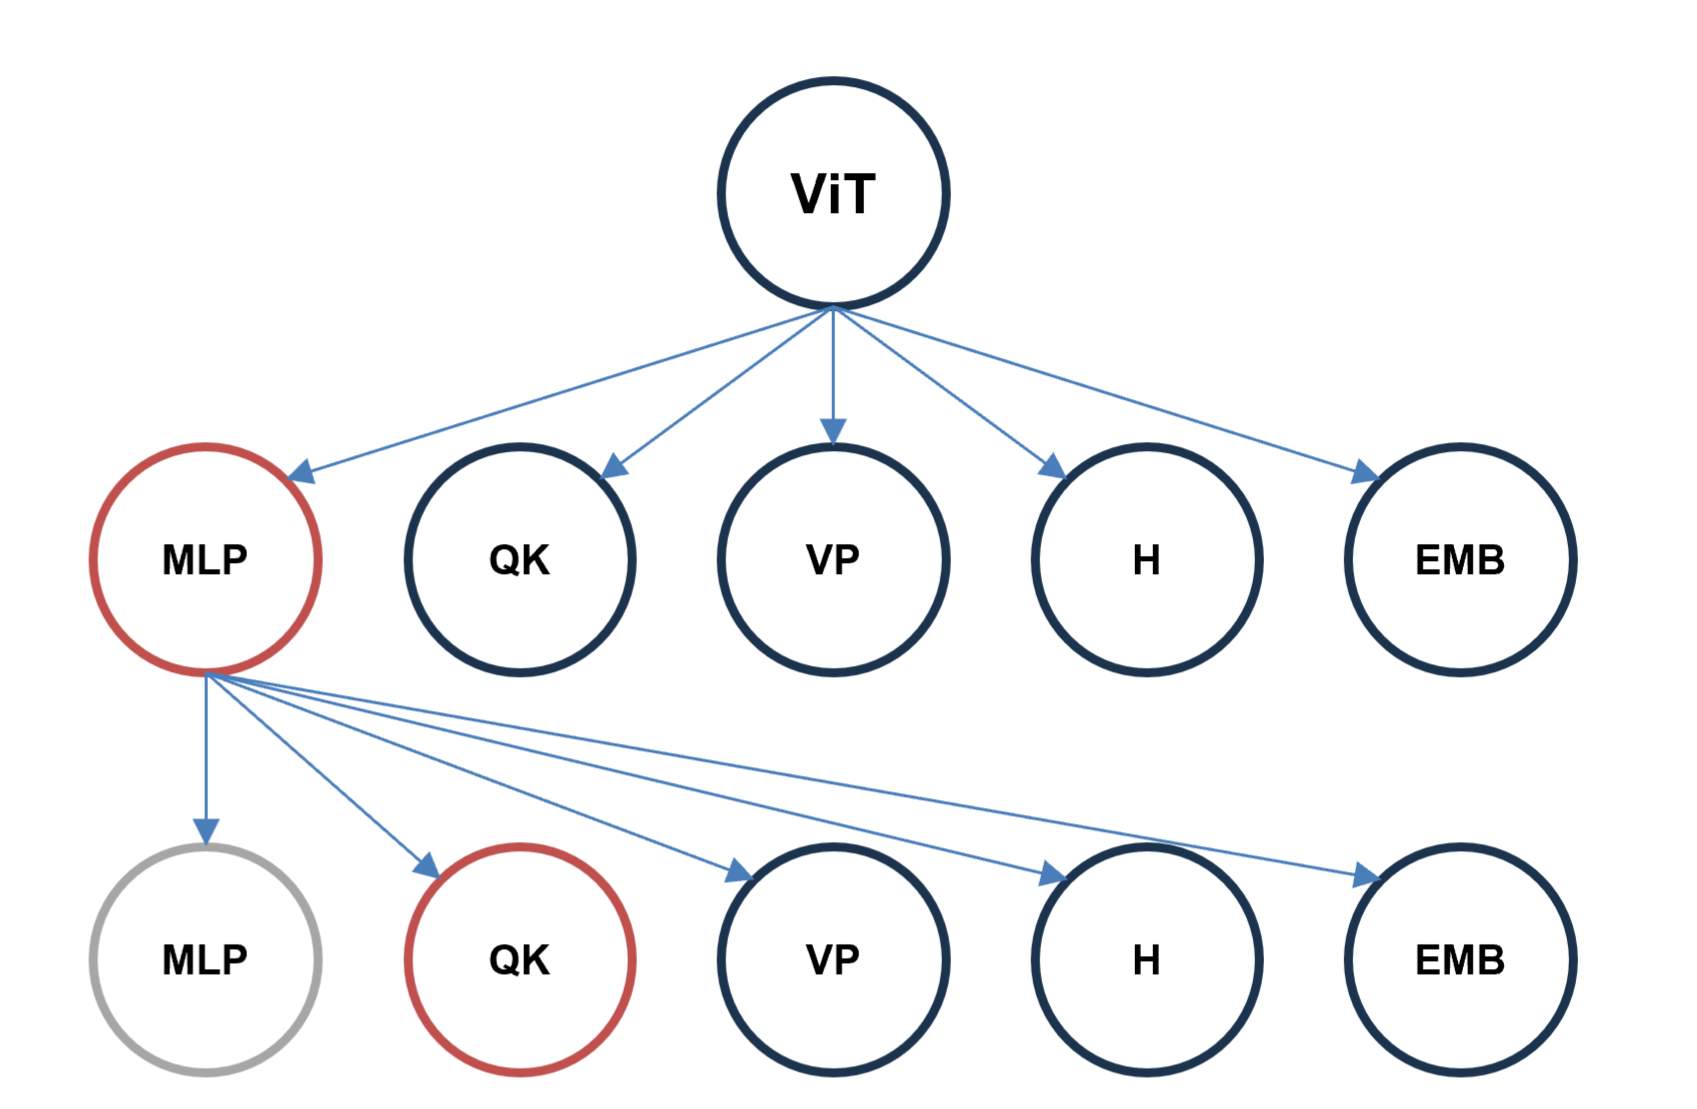
\includegraphics[width=0.75\textwidth]{images/SearchTree.png}
    \caption{Rappresentazione schematica dell'albero di ricerca generato dalle azioni di \textit{Branching}.}
\end{figure}
Attraverso il \textit{branching} viene costruito un \textbf{albero 5-ario} di ricerca, dove ogni nodo rappresenta una specifica \textit{Subnet} ottenuta a partire dal nodo genitore. Ad ogni nodo viene associato un valore della funzione obiettivo, calcolato valutando l'accuratezza su un ridotto set di immagini (\textit{Search Set}) (utilizzando esclusivamente i parametri attivi) e il relativo numero di parametri residui. Questo valore verrà successivamente utilizzato per verificare i vincoli di \textit{Bound} e, qualora risultasse più elevato del miglior valore individuato dalla ricerca, si aggiornerebbe quest'ultimo e si salverebbe la maschera di \textit{Pruning} corrispondente. \newline
Al fine di massimizzare l'efficacia del taglio dei parametri, la strategia di esplorazione \textit{Depth First} è stata scelta per favorire il raggiungimento dei nodi foglia dell'albero di ricerca. Questo permette all'algoritmo di individuare rapidamente configurazioni caratterizzate da un elevato numero di azioni di \textit{pruning} e, di conseguenza, da una significativa riduzione dei parametri.\newline
L'introduzione di un limite di profondità nell'albero di ricerca permette di mitigare l'impatto cumulativo del \textit{pruning} sulle prestazioni del modello. Un'esplorazione eccessivamente profonda comporterebbe infatti una rimozione massiva di parametri in un'unica iterazione, rischiando di degradare l'accuratezza in modo irreversibile. In tali scenari, il danno strutturale all'architettura potrebbe risultare troppo elevato, rendendo difficoltoso il recupero delle performance originali.

\subsection{Bound}
La dimensione dell'albero di ricerca risulta significativa; in particolare,
detta ${D}$ la massima profondità dell'albero e considerato che si tratta di un
albero 5-ario, il numero totale di nodi è pari a:

\begin{equation}
    {N} = \sum_{i=0}^{{D}} 5^i
\end{equation}

Ad esempio, se ${D} = 6$, il numero totale di nodi è pari a $19.531$.
Considerando che per ogni nodo è necessario calcolare i gradienti per tutti i
parametri attivi del modello al fine di stimarne l'importanza, il tempo
necessario per una ricerca esaustiva risulterebbe proibitivo. Tale criticità
viene risolta attraverso la fase di \textbf{Bound}, che permette di effettuare
un \textit{pruning on-the-fly} sull'albero di ricerca, escludendo interi rami
computazionalmente onerosi ma poco promettenti dal punto di vista della
funzione obiettivo. \newline In particolare, per ogni nodo $n$ esplorato, viene
verificato il seguente vincolo di ammissibilità:
\begin{equation}
    \text{Obj}(n) > \text{Obj}_{best} - \epsilon
\end{equation}
Qualora il vincolo venisse violato, il nodo non verrebbe sottoposto a \textit{Branching}, troncando di fatto l'esplorazione del suo sottoalbero. È importante sottolineare la presenza del \textbf{fattore di tolleranza}~$\epsilon$: esso consente alla ricerca di non arrestarsi prematuramente, permettendo l'esplorazione di subnet che, pur essendo leggermente inferiori al miglior valore individuato ($\text{Obj}_{best}$), si trovano in regioni dello spazio degli stati potenzialmente ottimali. Questo approccio garantisce una ricerca più robusta e completa, anche se maggiormente onerosa in termini computazionali.
\subsection{Ottimalità dell'algoritmo di ricerca}
Risulta importante sottolineare che il \textit{Branch and Bound} è un algoritmo
ottimo, come dimostrato da Lawler e Wood \cite{BnBOptim}. Tale garanzia di
ottimalità globale risiede nella definizione di un \textit{bound} che sia
\textbf{ammissibile}: in un problema di massimizzazione, il valore calcolato in
ogni nodo deve rappresentare un limite superiore (\textit{upper bound})
insuperabile per qualsiasi sottoproblema derivato da quel nodo. Formalmente,
detto $S$ l'insieme delle soluzioni nel sotto-albero del nodo $n$, il bound è
ammissibile se:
\begin{equation}
    \text{Obj}(n) \geq \max_{x \in S} \text{Obj}(x)
\end{equation}
dove $\text{Obj}(x)$ è la funzione
obiettivo. Solo sotto questa condizione l'azione di \textit{pruning} non
rischia di escludere l'ottimo globale. Tuttavia, nel contesto della presente
ricerca, l'applicazione del \textit{Branch and Bound} assume una natura più
euristica per due ragioni fondamentali:
\begin{enumerate}
    \item \textbf{Assenza di un limite superiore teorico:} La funzione obiettivo utilizzata non è intrinsecamente monotona rispetto alla profondità dell'albero. La riduzione dei parametri aumenta con la profondità ma l'accuratezza risulta variabile e non strettamente correlata a quest'ultima, non permettendo quindi di calcolare un \textit{bound} che sia un limite superiore certo per ogni possibile combinazione futura.
    \item \textbf{Introduzione di una soglia di tolleranza:} Al fine di accelerare l'esplorazione di uno spazio degli stati altrimenti intrattabile, è stata introdotta una soglia $\epsilon$ nelle condizioni di \textit{pruning}. Questa scelta trasforma l'algoritmo in un metodo di ricerca \textbf{$\epsilon$-ottimo}, che garantisce l'identificazione di una soluzione entro un margine di errore controllato rispetto all'ottimo teorico, ma privilegia drasticamente la velocità di convergenza.
\end{enumerate}
In conclusione, sebbene si rinunci alla garanzia di ottimalità assoluta definita in letteratura~\cite{BnBOptim}, l'algoritmo così configurato permette di navigare efficacemente il complesso \textit{trade-off} tra performance e dimensione del modello, individuando \textit{Subnet} di alta qualità che una ricerca esaustiva non avrebbe potuto identificare in tempi ragionevoli.

\section{Formulazione delle Azioni di ricerca}
\label{section:math_actions}
Per ogni nodo dell'albero di ricerca, l'applicazione delle azioni di
\textit{pruning} genera i cinque nodi figli corrispondenti. Ciascuna azione
identifica un gruppo specifico di parametri ${W}_g$ all'interno
dell'architettura che può essere rimosso minimizzando il degrado delle
prestazioni del modello. \par
Al fine di individuare le componenti meno rilevanti per le capacità predittive
del modello, viene adottata una metrica di importanza basata sulla sensibilità
della funzione di perdita rispetto ai parametri. Per un singolo parametro $w$,
l'importanza è definita come:
\begin{equation} \label{eq:metrica_importanza}
    {\mathbb{I}}(w) = w^2 \cdot \mathbb{E}_{x \sim {D}} \left[ \left( \frac{\partial {L}(x; \theta^*)}{\partial w} \right)^2 \right],
\end{equation}
dove ${L}(x; \theta^*)$ è la funzione di perdita, calcolata a partire dai parametri attivi $\theta^*$, sui campioni~$x$ (\textit{Search Set}).
Si è scelto di adottare una tipologia di \textit{pruning strutturato}, di conseguenza è necessario definire l'importanza di un intero gruppo di parametri ${W}_g$ (come un intero neurone, dove ${W}_g = \{w_1, w_2, \ldots, w_K, b\}$, considerato $y = \sum_{i=1}^{K} w_i x_i + b$) che viene calcolata come la somma dei contributi individuali:
\begin{equation}
    {\mathbb{I}}({W}_g) = \sum_{w \in {W}_g} {\mathbb{I}}(w).
\end{equation}

Le specifiche azioni di \textit{pruning} possono essere definite come un
problema di minimizzazione locale volto a identificare il gruppo di dimensioni
(formate da più parametri) $g$ la cui rimozione minimizza l'impatto sulla
funzione di perdita ${L}$. Per garantire la compatibilità tra il modello
compresso e l'hardware pensato per l'accelerazione di questi modelli (Tensor
Core \cite{TensorCores}), imponiamo un vincolo di cardinalità $|g| = K$ (con
$K$ multiplo di 8). In tal modo è possibile definire il metodo proposto come
\textbf{Hardware-Aware Pruning}. Di seguito la formulazione matematica
dettagliata per ogni azione:

\raggedbottom{
    \begin{itemize}
        \item \textbf{Pruning MLP:} Sia ${B}$ l'insieme dei blocchi \textit{Transformer} e \mbox{$\mathrm{MLP}_{b_i}= \{ g \subset W_{\mathrm{MLP}, b_i} : |g| = K \}$} l'insieme dei possibili raggruppamenti di cardinalità $K$ di dimensioni del modulo MLP nel blocco $i$-esimo $b_i$. L'azione identifica il gruppo $g^*_{\mathrm{MLP}}$ che minimizza:
              \begin{equation}
                  g^*_{\mathrm{MLP}} = \arg\min_{\substack{b_i \in {B} \\ g_{K} \in \mathrm{MLP}_{b_i}}} \sum_{W_g \in g_{K}} {\mathbb{I}}(W_g).
              \end{equation}
              Come è possibile notare dalla figura \ref{figure:MLP} l'azione di \textit{Pruning MLP} comporta la rimozione di $K$ colonne di pesi, non necessariamente contigue, dalle matrici dei parametri del modulo \textit{Multi-Layer Perceptron} del blocco $i$-esimo $b_i$.
              \begin{figure}[ht]
                  \centering
                  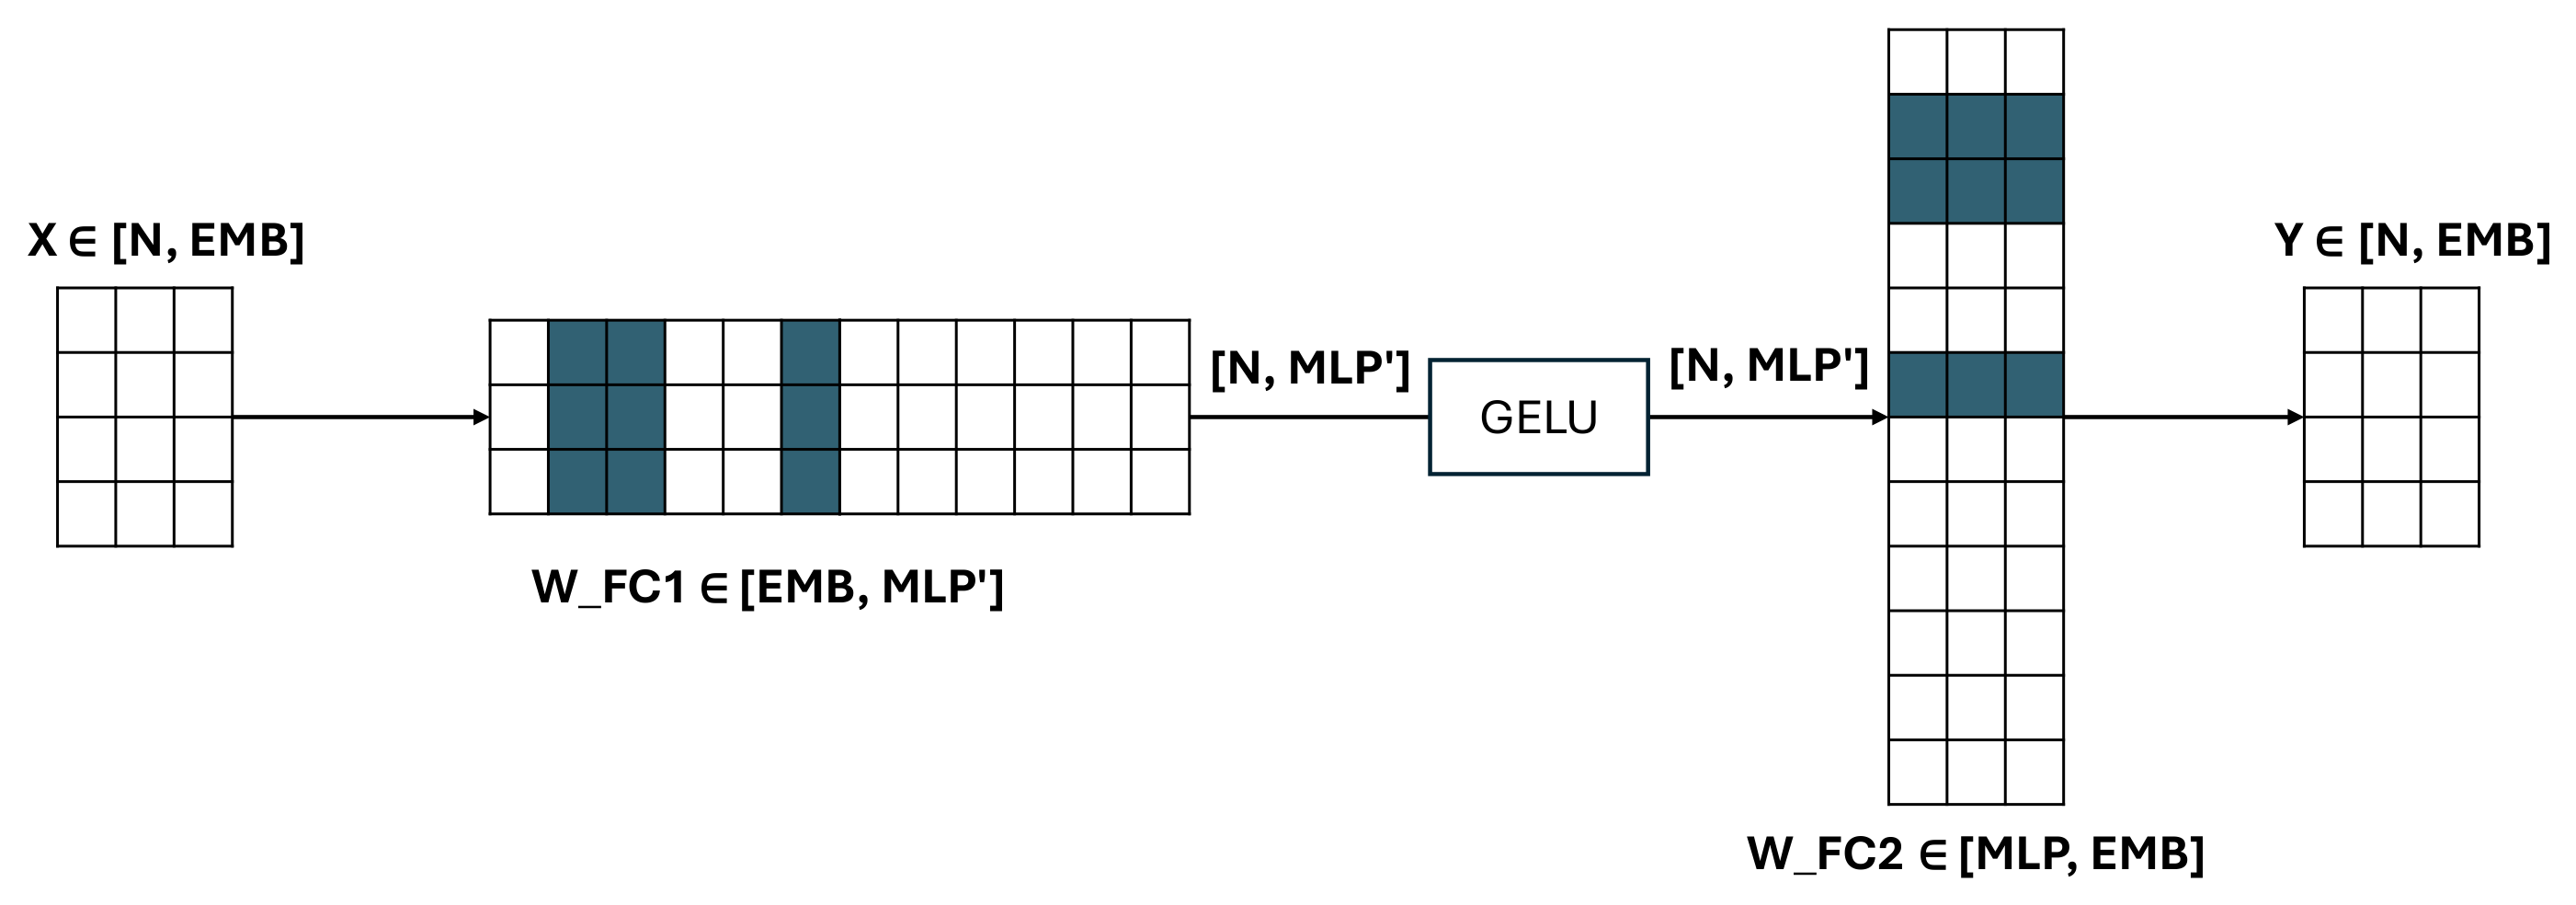
\includegraphics[width=0.75\textwidth]{images/Pruning/MlpPruning.png}
                  \caption{Visualizzazione delle matrici dei pesi mascherate dall'azione di \textit{MLP Pruning}.}
                  \label{figure:MLP}
              \end{figure}

        \item \textbf{Pruning QK (Query-Key):} Sia ${B}$ l'insieme dei blocchi \textit{Transformer} e \newline\mbox{$\mathrm{QK}_{b_i}= \{ g \subset {W}_{\mathrm{QK}, b_i} : |g| = K \}$} l'insieme dei raggruppamenti di $K$ dimensioni condivise tra i moduli Query e Key di tutte le teste di attenzione del blocco $i$-esimo. L'azione identifica il gruppo $g^*_{\mathrm{QK}}$ che minimizza:
              \begin{equation}
                  g^*_{\mathrm{QK}} = \arg\min_{\substack{b_i \in {B} \\ g_{K} \in \mathrm{QK}_{b_i}}} \sum_{W_g \in g_{K}} {\mathbb{I}}(W_g).
              \end{equation}
              Notare che le dimensioni dei moduli Query e Key vengono rimosse contestualmente a tutte le teste di attenzione del blocco $i$-esimo $b_i$. Questo è particolarmente evidente nella figura \ref{figure:QK}, ed è necessario per mantenere la consistenza matematica delle dimensioni delle matrici.
              \begin{figure}[ht]
                  \centering
                  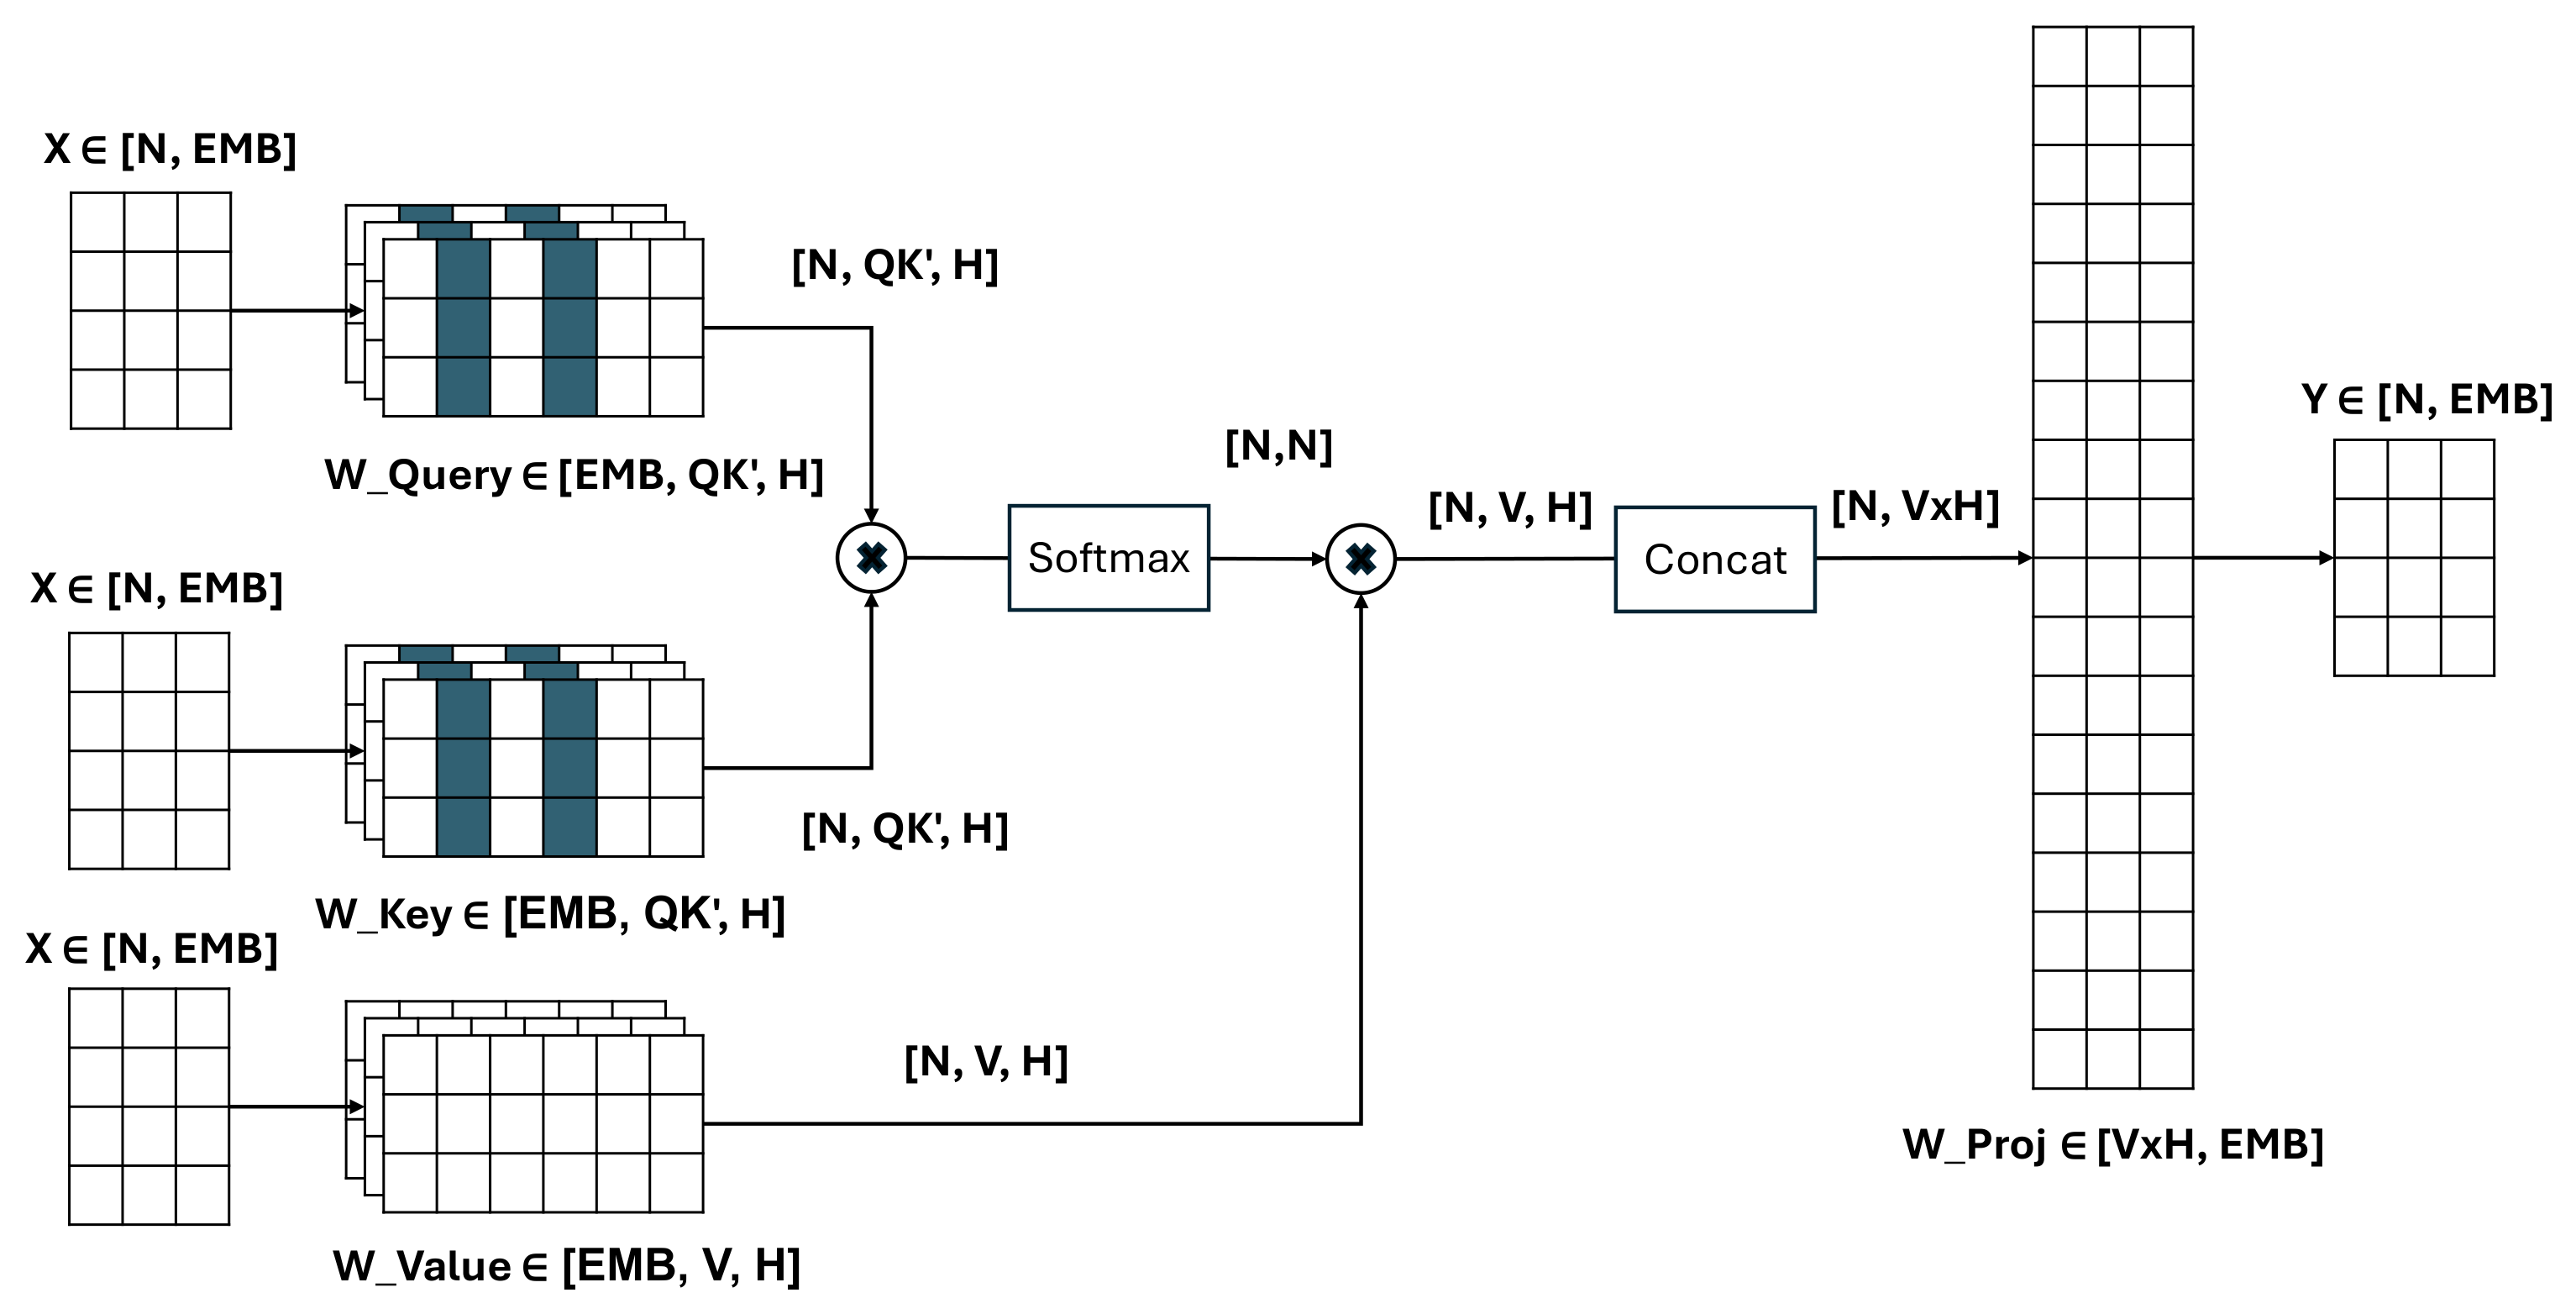
\includegraphics[width=0.75\textwidth]{images/Pruning/QKpruning.png}
                  \caption{Visualizzazione delle matrici dei pesi mascherate dall'azione di \textit{QK Pruning}, nella \textit{MHSA}.}
                  \label{figure:QK}
              \end{figure}

        \item \textbf{Pruning VPROJ (Value-Projection):} Sia ${B}$ l'insieme dei blocchi \textit{Transformer} e \newline
              \mbox{$\mathrm{VP}_{b_i}= \{ g \subset {W}_{\mathrm{VP}, b_i} : |g| = K \}$} l'insieme dei raggruppamenti di cardinalità $K$ di dimensioni dei moduli \textit{Value} e \textit{Output Projection} di tutte le teste di attenzione nel blocco $i$-esimo. L'azione identifica il gruppo $g^*_{\mathrm{VP}}$ che minimizza:
              \begin{equation}
                  g^*_{\mathrm{VP}} = \arg\min_{\substack{b_i \in {B} \\ g_{K} \in \mathrm{VP}_{b_i}}} \sum_{W_g \in g_{K}} {\mathbb{I}}(W_g).
              \end{equation}
              Come è possibile osservare dalla figura \ref{figure:VProj}, l'azione di \textit{Pruning VProj} comporta la rimozione di $K$ colonne di pesi, non necessariamente contigue, dalle matrici dei parametri dei moduli \textit{Value} e \textit{Output Projection} di tutte le teste di attenzione del blocco $i$-esimo $b_i$. Questo per le stesse ragioni di consistenza matematica delle dimensioni viste per il \textit{Pruning QK}.
              \begin{figure}[ht]
                  \centering
                  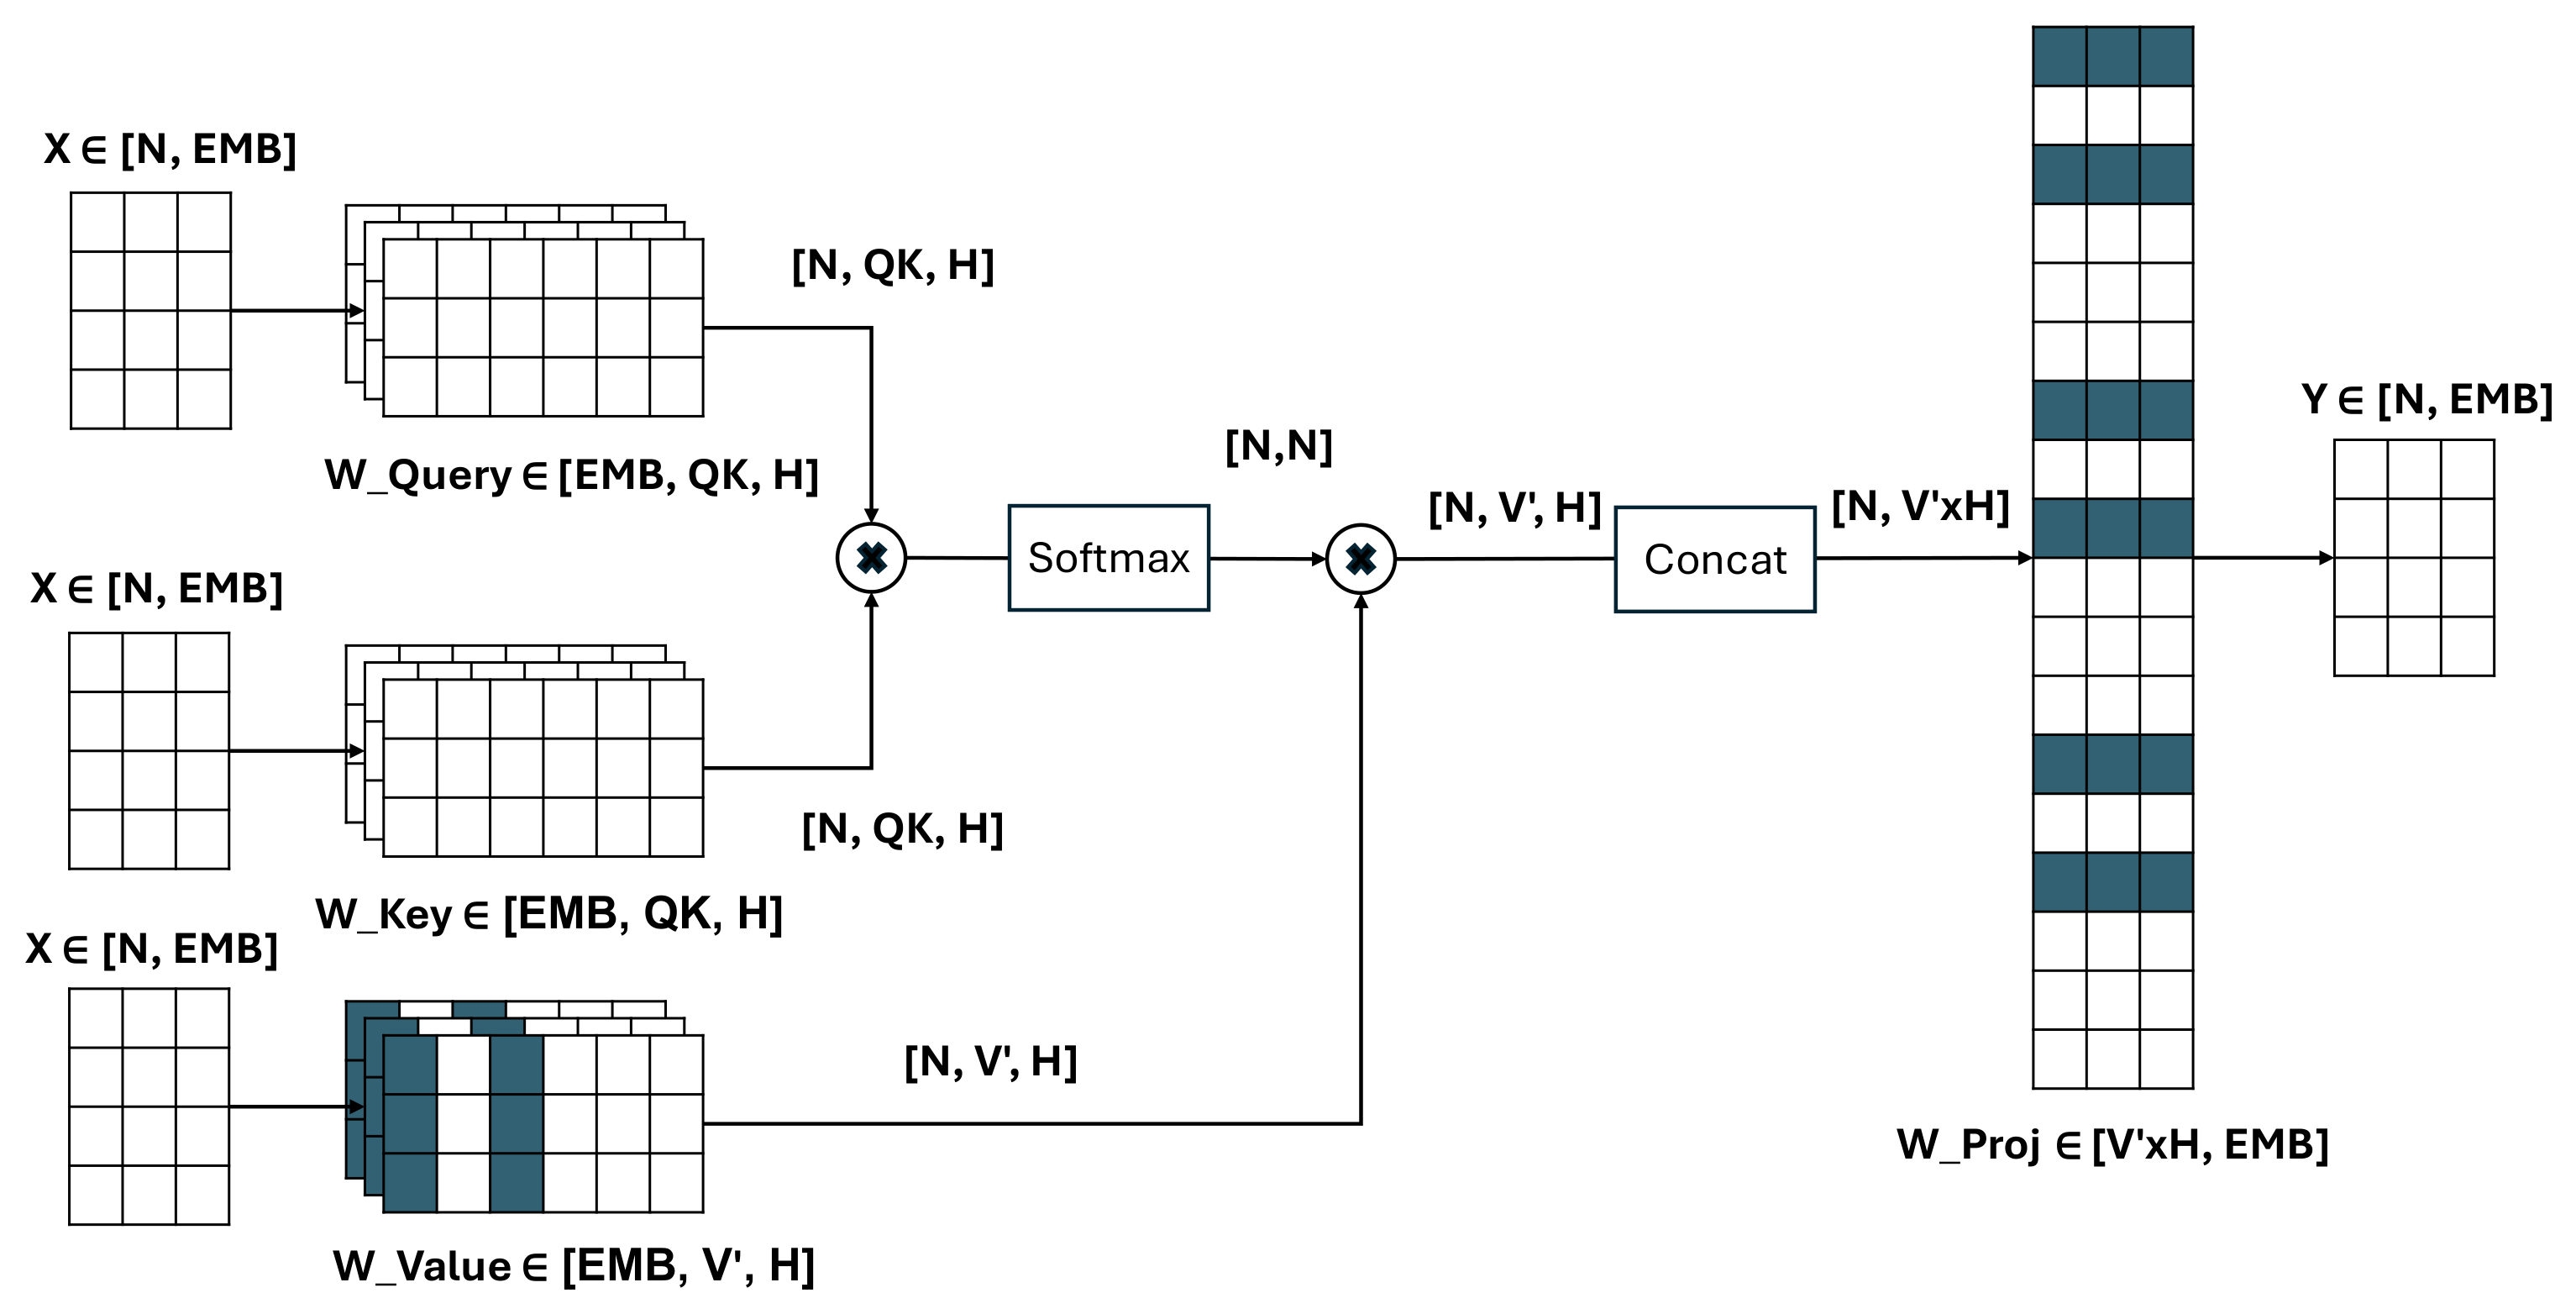
\includegraphics[width=0.75\textwidth]{images/Pruning/VProjPruning.png}
                  \caption{Visualizzazione delle matrici dei pesi mascherate dall'azione di \textit{VProj Pruning}, nella \textit{MHSA}.}
                  \label{figure:VProj}
              \end{figure}

        \item \textbf{Pruning HEAD:} Sia ${B}$ l'insieme dei blocchi \textit{Transformer} e $H_{b_i}$ l'insieme di tutte le teste di attenzione nel blocco $i$-esimo. L'azione identifica la head $h^*$ che minimizza:
              \begin{equation}
                  h^* = \arg\min_{\substack{b_i \in {B} \\ h \in H_{b_i}}} \sum_{W_g \in h} {\mathbb{I}}(W_g).
              \end{equation}
              L'azione di \textit{Pruning Head} comporta la rimozione completa di una testa di attenzione, ovvero la mascheratura di tutte le dimensioni dei moduli Query, Key, Value e Output Projection associati alla head $h^*$ in tutte le matrici dei parametri del blocco $i$-esimo $b_i$. Questo è particolarmente evidente nella figura \ref{figure:Head}.
              \begin{figure}[ht]
                  \centering
                  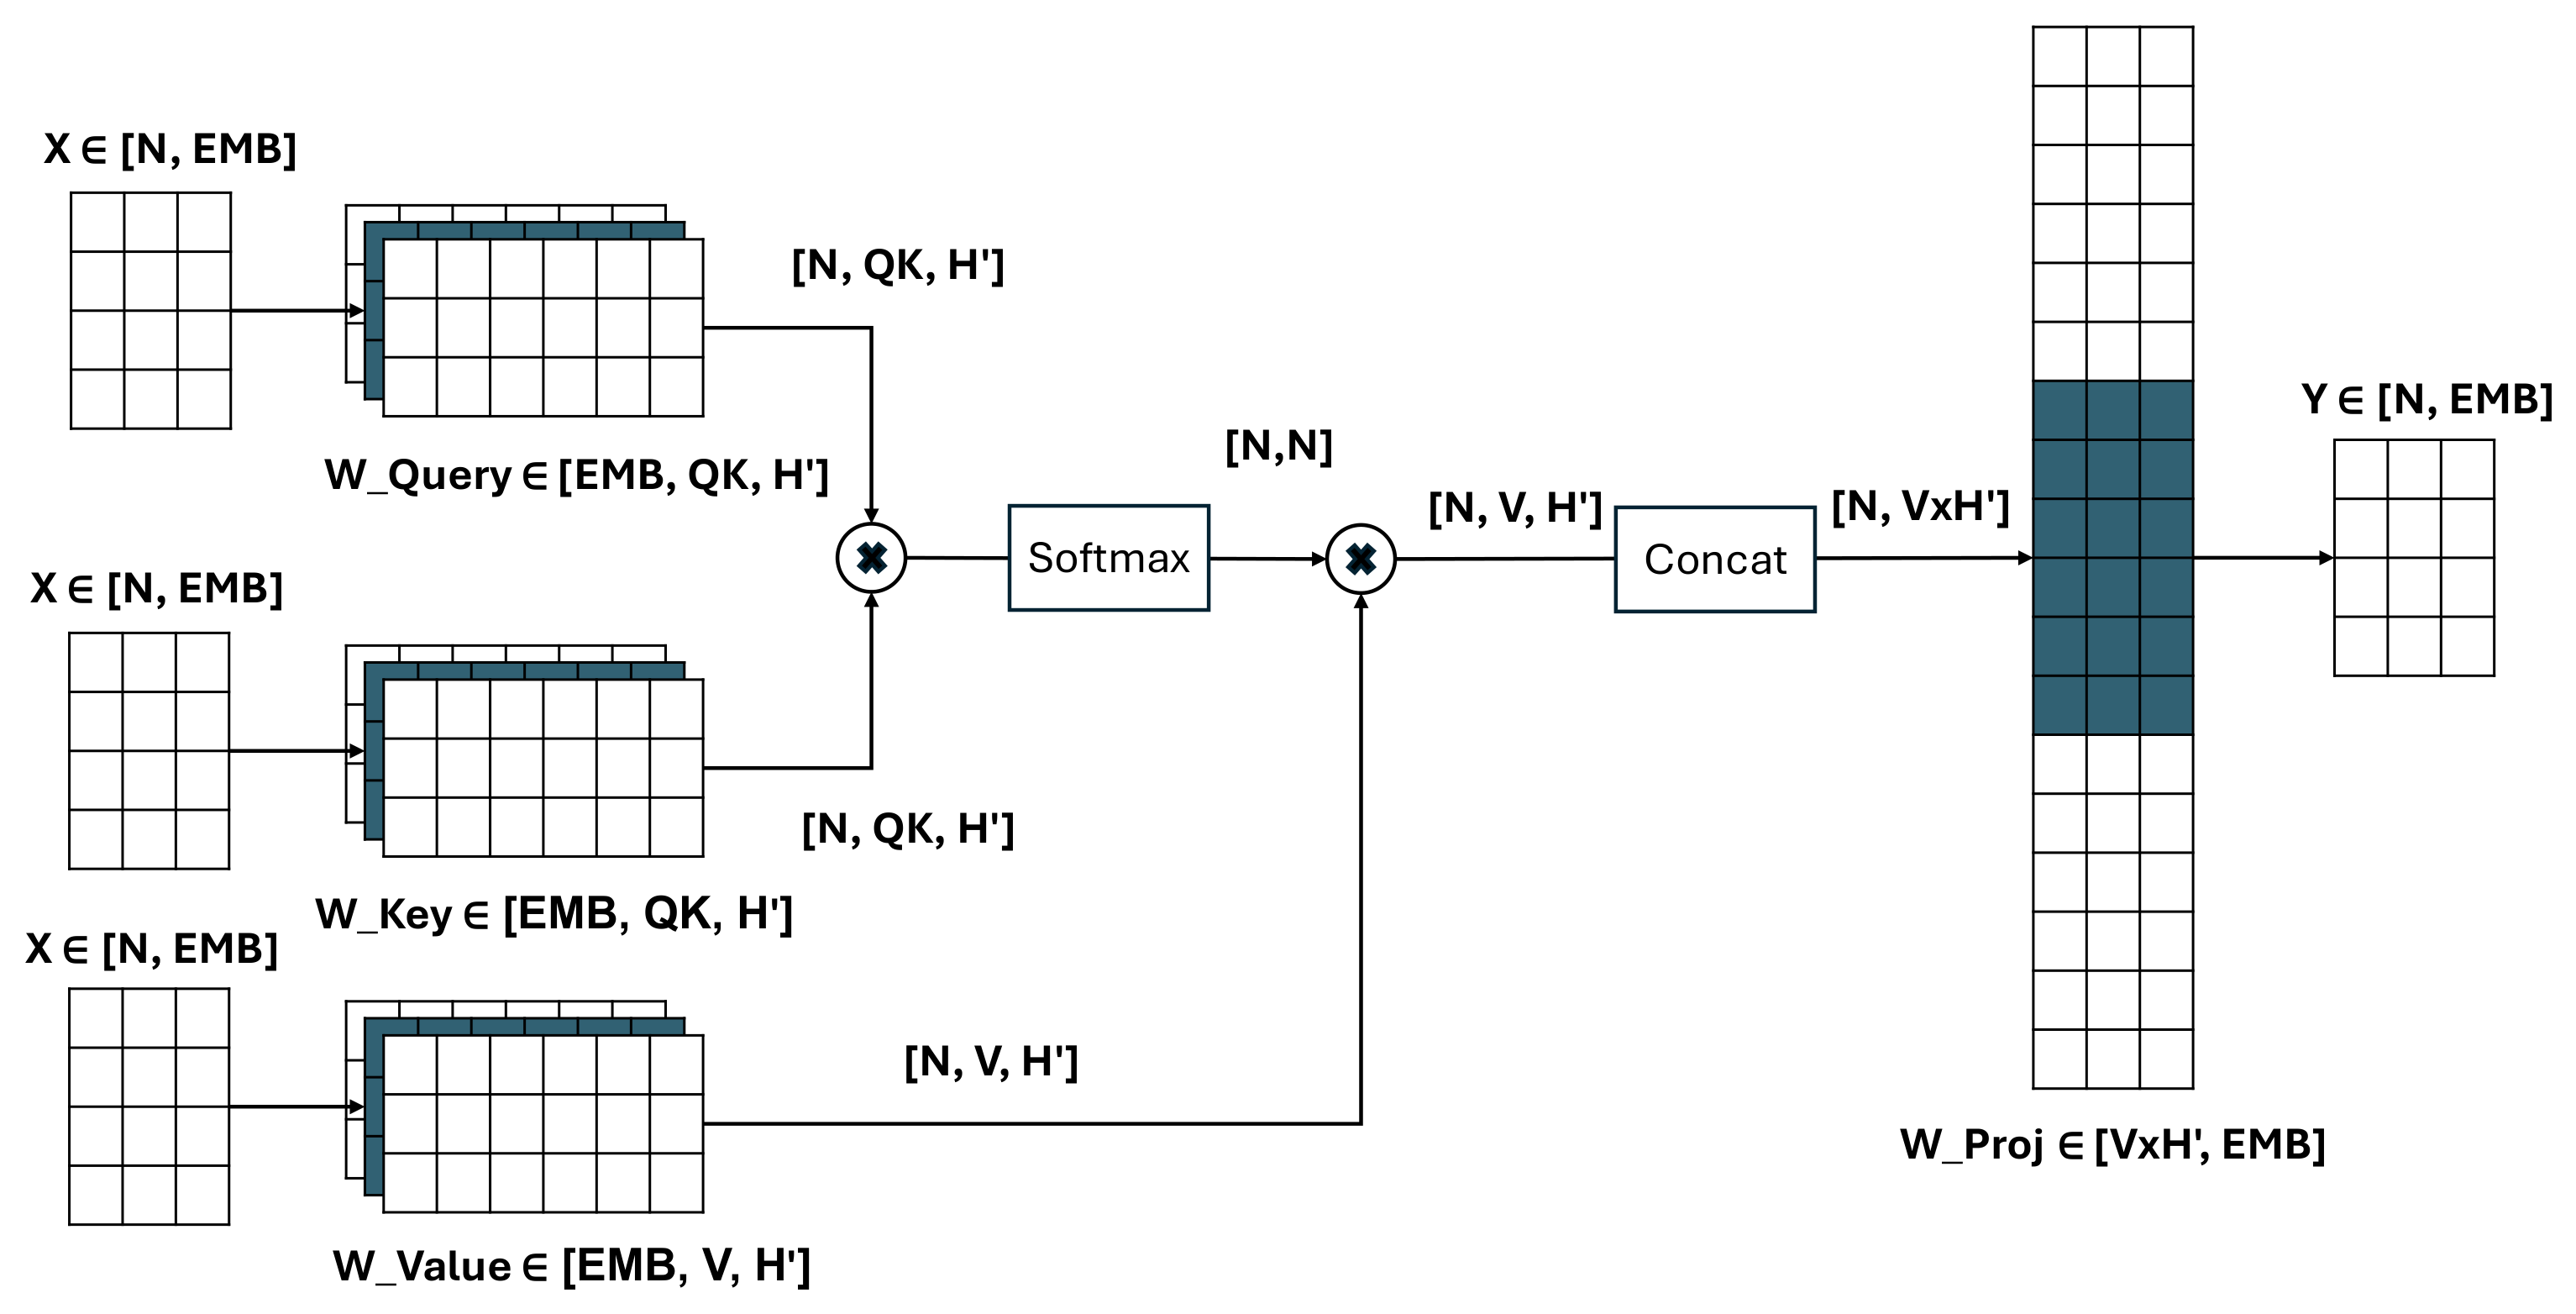
\includegraphics[width=0.75\textwidth]{images/Pruning/HeadPruning.png}
                  \caption{Visualizzazione delle matrici dei pesi mascherate dall'azione di \textit{Head Pruning}, nella \textit{MHSA}.}
                  \label{figure:Head}
              \end{figure}

        \item \textbf{Pruning EMB (Embedding):} Sia $\mathrm{EMB}= \{ g \subset {W}_{\mathrm{EMB}} : |g| = K \}$ l'insieme di tutti i raggruppamenti di cardinalità $K$ di dimensioni dell'\textit{Embedding} nell'intero modello \textit{Transformer}. L'azione identifica il gruppo $g^*_{\mathrm{EMB}}$ che minimizza:
              \begin{equation}
                  g^*_{\mathrm{EMB}} = \arg\min_{g_{K} \in \mathrm{EMB}} \sum_{W_g \in g_{K}} {\mathbb{I}}(W_g)
              \end{equation}
              Si noti che, a differenza delle azioni precedenti, il \textit{Pruning} dell'\textit{Embedding} opera sulla dimensione globale del modello. La rimozione di un raggruppamento $g_{K}$ in questa fase comporta una potatura della rappresentazione vettoriale che si propaga attraverso l'intera architettura, influenzando la dimensione di tutti i blocchi \textit{Transformer}. Infine è importante osservare che questa azione comporta una eliminazione di righe delle matrici dei parametri sia nella \textit{MHSA} che nella \textit{FFN}, come è possibile notare dalle figure \ref{figure:MHSA-emb} e \ref{figure:FFN-emb}.
              \begin{figure}[H]
                  \centering
                  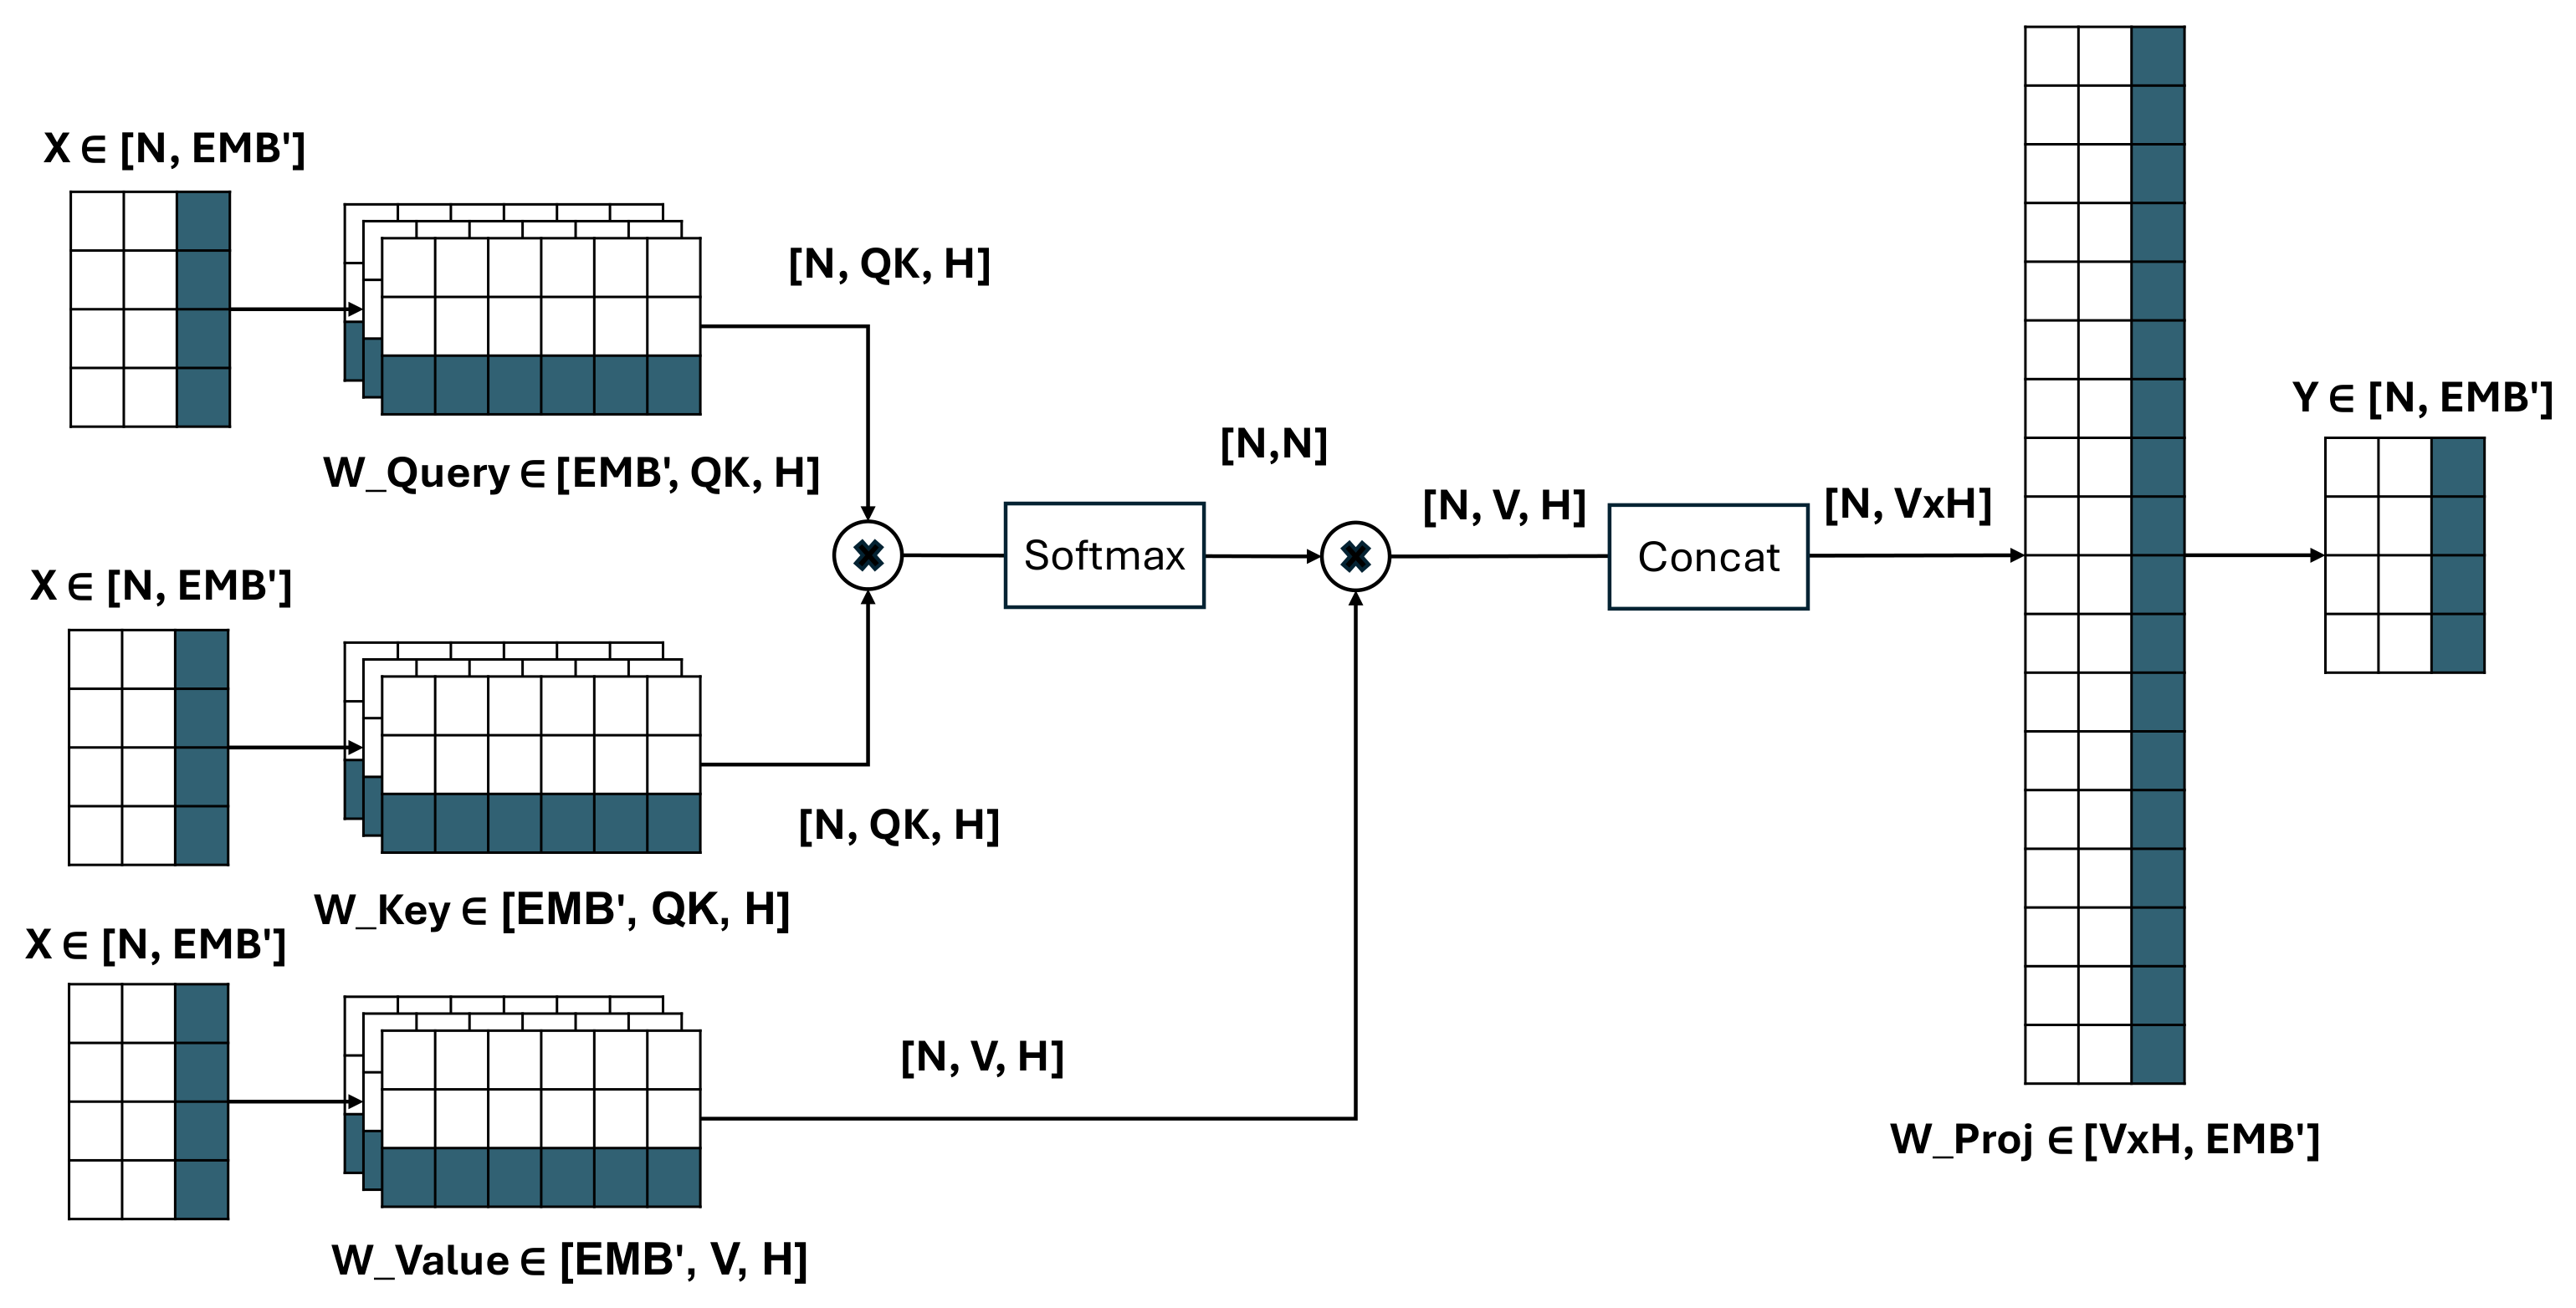
\includegraphics[width=0.75\textwidth]{images/Pruning/EmbMHSAPruning.png}
                  \caption{Visualizzazione delle matrici dei pesi mascherate dall'azione di \textit{Emb Pruning}, nella \textit{MHSA}.}
                  \label{figure:MHSA-emb}
              \end{figure}
              \begin{figure}[H]
                  \centering
                  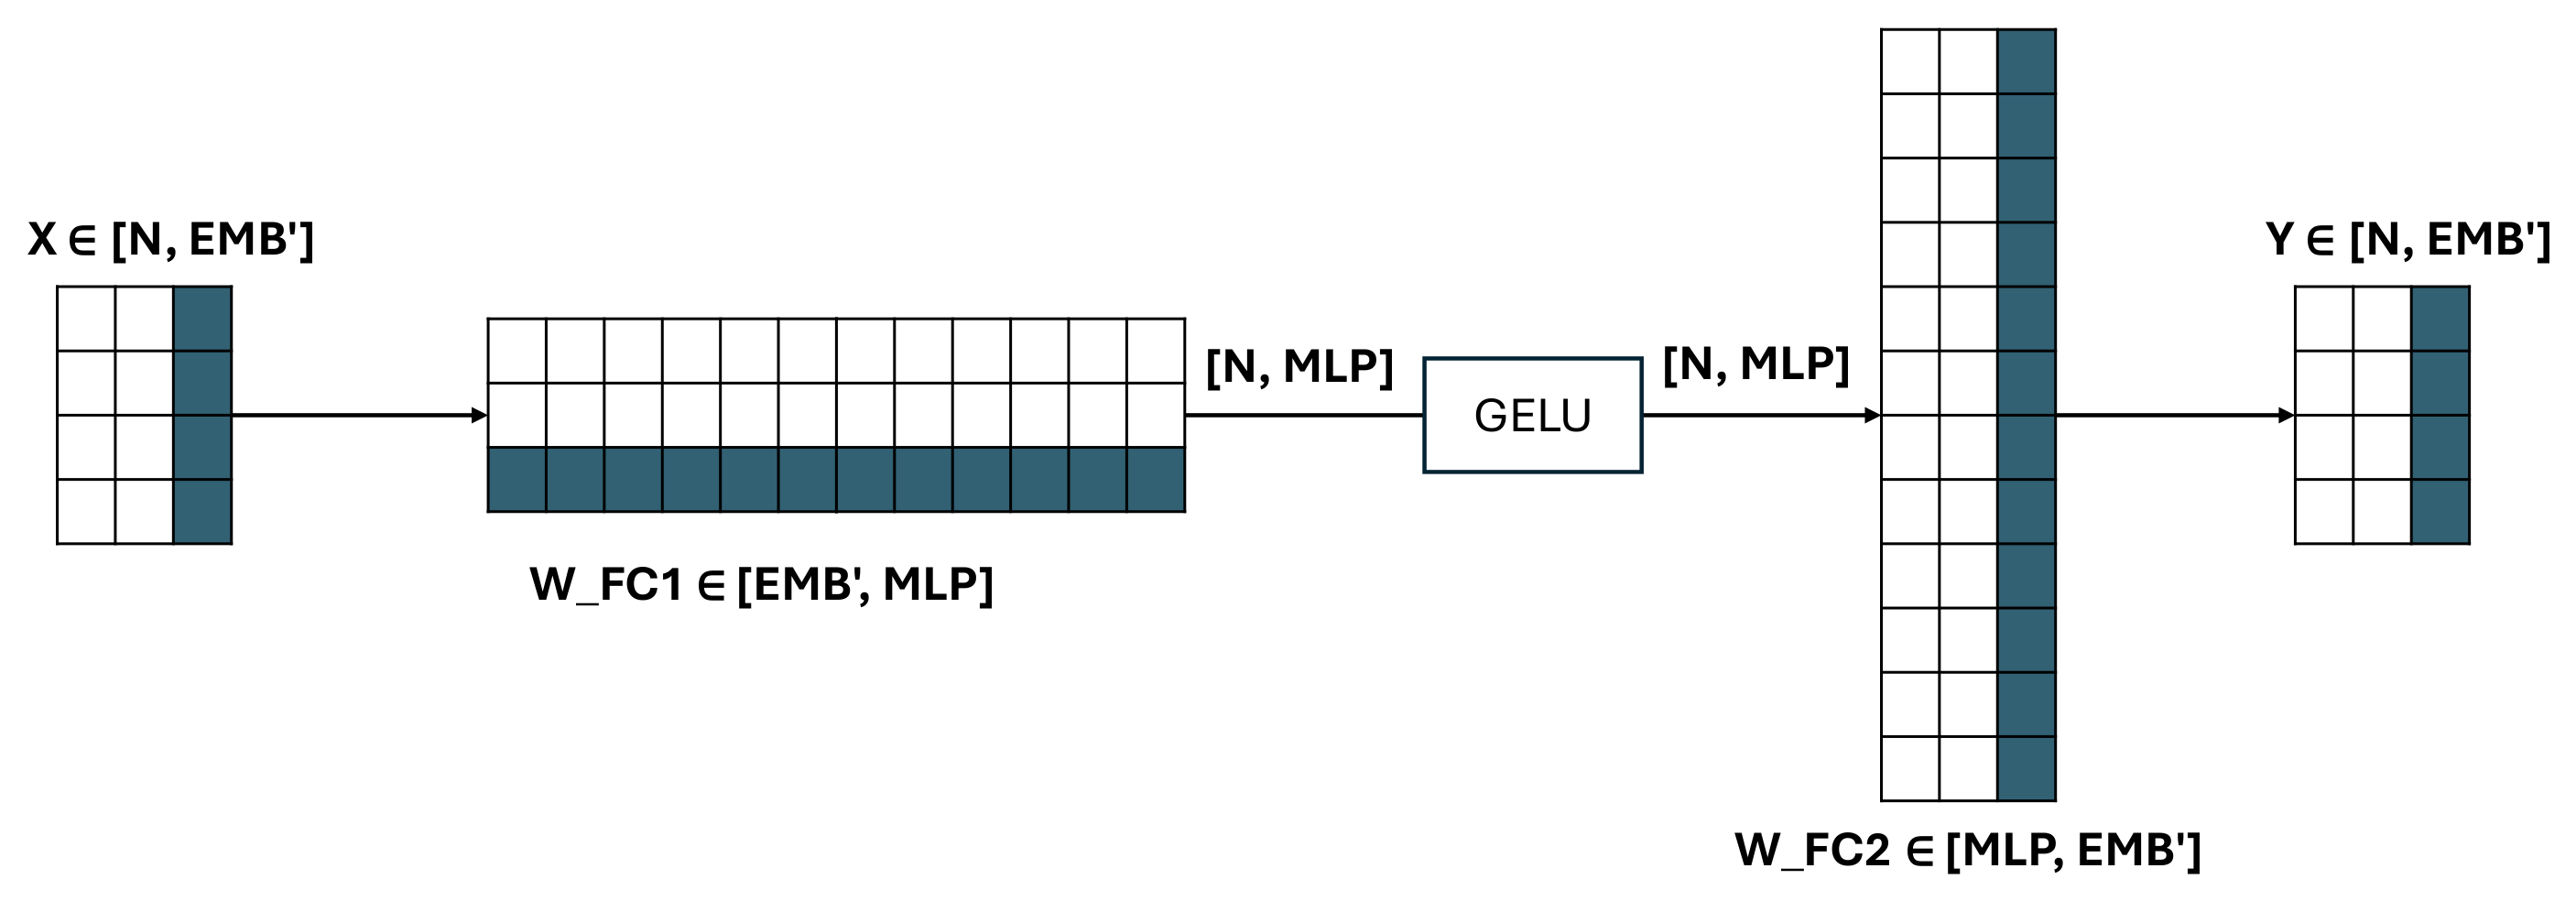
\includegraphics[width=0.75\textwidth]{images/Pruning/EmbMlpPruning.png}
                  \caption{Visualizzazione delle matrici dei pesi mascherate dall'azione di \textit{Emb Pruning}, nella \textit{FFN}.}
                  \label{figure:FFN-emb}
              \end{figure}
    \end{itemize}
}

\section{Derivazione del criterio di importanza}
La metrica di importanza utilizzata combina le informazioni sulla magnitudo dei
pesi e dei gradienti, al fine di misurare la sensibilità di uno specifico
parametro a partire dai dati in input al modello. I parametri meno sensibili
vengono interpretati come di scarso contributo all'output del modello, e di
conseguenza vengono rimossi. La derivazione della metrica di importanza
considera un singolo parametro $w$ e il suo effetto sulla funzione di perdita
$L$. In particolare si analizza la variazione di $L$ al variare di $w$:
\begin{equation}
    \Delta L = L(w + \delta w) - L(w),
\end{equation}
\begin{equation}
    L(w + \delta w) = L(w) + \Delta L.
\end{equation}

Per approssimare il valore della funzione di perdita con il nuovo valore del
parametro $L(w + \delta w)$ si utilizza l'espansione di Taylor al primo ordine:
\begin{equation}
    L(w + \delta w) \approx L(w) + \frac{\partial L}{\partial w} \cdot \delta w + {o}(\delta{w}).
\end{equation}

Dato che l'operazione effettuata è la potatura, il valore del parametro
perturbato è zero (in quanto viene tagliato) e di conseguenza $\delta w = -w$,
da cui possiamo ottenere il valore approssimato della variazione di $L$:
\begin{equation}
    L(w + \delta w) - L(w) \approx (-w) \cdot \frac{\partial L}{\partial w}.
\end{equation}

Applicato ad un gruppo di parametri $W_g$ (ad esempio un intero neurone):
\begin{equation}
    \Delta L(W_g) = \sum_{w \in W_g} \Delta L(w) = \sum_{w \in W_g} -w \cdot \frac{\partial L}{\partial w} = - \sum_{w \in W_g} w \cdot \frac{\partial L}{\partial w}.
\end{equation}

Nonostante l'approssimazione al primo ordine sia ampiamente sfruttata in
letteratura \cite{Metrics} per la sua semplicità computazionale, essa introduce
un rischio sistematico nel caso del pruning strutturato. Si consideri un gruppo
di parametri $W_g$ contenente due parametri $w_1$ e $w_2$. Nell'eventualità in
cui le variazioni individuali della perdita siano opposte, ovvero \mbox{$\Delta
        L(w_1) \approx - \Delta L(w_2)$}, la loro somma algebrica risulterebbe prossima
allo zero:
\begin{equation}
    \Delta L(W_g) = \Delta L(w_1) + \Delta L(w_2) \approx 0.
\end{equation}
Tale risultato porterebbe l'algoritmo a classificare erroneamente il gruppo $W_g$ come irrilevante, ma in realtà è possibile che i singoli parametri possiedano un'elevata sensibilità. Poiché $\Delta L$ è una stima lineare e locale della reale superficie della funzione di perdita, fare affidamento sulla somma con segno dei contributi espone a decisioni di taglio errate, dove componenti critiche vengono rimosse a causa di una reciproca compensazione dei gradienti. \par
La soluzione a questo problema può essere individuata in un approccio più
conservativo, utilizzando i quadrati per permettere la somma dei contributi
individuali (che saranno così sempre positivi):
\begin{equation}
    {\mathbb{I}}(W_g) = \sum_{w \in W_g} \Delta L(w)^2 = \sum_{w \in W_g} \left ( w \cdot \frac{\partial L}{\partial w}\right )^2.
\end{equation} \newline
Notare che il calcolo del gradiente $\frac{\partial L}{\partial w}$ non è banale. Infatti accumulando semplicemente i gradienti, si rischia di incorrere in un fenomeno di cancellazione. Ad esempio detti $b_1$ e $b_2$ i due (unici) \textit{batch} di dati in input, potrebbe accadere che:
\begin{equation}
    \frac{\partial L}{\partial w}(b_1) \approx - \frac{\partial L}{\partial w}(b_2).
\end{equation}
In fase di accumulo questo fenomeno porterebbe a un gradiente complessivo circa nullo, azzerando erroneamente l'importanza del parametro. \par
La soluzione a questo problema può essere facilmente individuata nell'utilizzo
del valore atteso del gradiente sui batch, da cui:
\begin{equation}
    {\mathbb{I}}(w) = w^2 \cdot \mathbb{E}_{b \sim {D}}\left [\left(\frac{\partial L}{\partial w}(b)\right)^2\right ] = w^2 \cdot \frac{1}{N} \sum_{i=1}^{N} \left (\frac{\partial L}{\partial w}(b) \right)^2 \quad,
\end{equation}
con $N$ numero di \textit{batch} in input. \par
Date queste premesse, è possibile definire la seguente metrica di importanza
per un gruppo di parametri $W_g$:
\begin{equation}
    {\mathbb{I}}(W_g) =\sum_{w \in W_g} w^2 \cdot \mathbb{E}_{b \sim {D}} \left[ \left( \frac{\partial L(b)}{\partial w} \right)^2 \right].
\end{equation}

\section{Fisher Information Matrix ed Hessiano}
La metrica di importanza derivata nella sezione precedente combina
l'informazione fornita dalla magnitudo dei parametri con l'approssimazione
diagonale della \textbf{Matrice di Informazione di Fisher}
\cite{molchanov2019importanceestimationneuralnetwork,
    theis2018fastergazepredictiondense}, così definita:
\begin{equation}
    F(w) = \mathbb{E}_{x,y} \left[ \nabla L(y, f(x,w)) \cdot \nabla L(y, f(x,w))^T \right] \in \mathbb{R}^{|w| \times |w|},
\end{equation}
nella quale i singoli elementi rappresentano la correlazione tra i gradienti dei singoli parametri:
\begin{equation}
    F(w_i, w_j) = \mathbb{E}_{x,y} \left[ \frac{\partial L}{\partial w_i} \cdot \frac{\partial L}{\partial w_j} \right].
\end{equation}
Data la cardinalità dei parametri nei modelli \textit{Transformer}, il calcolo e la memorizzazione della matrice completa risultano computazionalmente proibitivi. Si assume pertanto l'indipendenza tra i parametri, operazione che equivale a considerare non nulla esclusivamente la diagonale della matrice:
$$ F(w_i, w_j) = 0 \quad \text{ed} \quad F(w_i, w_i) = \mathbb{E}_{x,y} \left[ \left(\frac{\partial L}{\partial w_i} \right)^2 \right]. $$
Empiricamente tale valore, detto \textbf{Informazione di Fisher}, viene stimato tramite una semplice media su un numero $N$ di \textit{batch} ($x_k$) in input:
\begin{equation}
    F(w) = \frac{1}{N} \sum_{k=1}^{N} \left( \frac{\partial L(x_k)}{\partial w} \right)^2.
\end{equation}
Notare che esiste un profondo legame tra l'\textit{Informazione di Fisher} e l'\textit{Hessiano} della funzione di perdita. A una simile conclusione sono giunti anche Theis et al. \cite{theis2018fastergazepredictiondense}. Di seguito la dimostrazione formale di questo legame, assumendo che la funzione di perdita sia la \textit{Negative Log-Likelihood}. \par
Consideriamo un problema di classificazione in cui il modello definisce una
distribuzione di probabilità $p(y|x,W)$. Per la proprietà di normalizzazione,
la somma delle probabilità su tutte le classi $y \in Y$ è unitaria:
\begin{equation}
    \sum_{y \in Y} p(y|x,W) = 1.
\end{equation}
Derivando rispetto ai parametri $W$ e sfruttando la linearità del gradiente:
\begin{equation}
    \sum_{y} \nabla_W p(y|x,W) = 0.
\end{equation}
Utilizzando una semplice proprietà delle derivate, per cui $\nabla p = p \frac{\nabla p}{p} = p \nabla \log(p)$, possiamo riscrivere l'espressione come:
\begin{equation}
    \sum_{y} p(y|x,W) \cdot \nabla_W \log p(y|x,W) = 0.
\end{equation}
Per brevità di notazione, assumiamo $p(y|x,W) = p(y)$ e deriviamo nuovamente rispetto a $W$:
\begin{equation}
    \nabla_W \sum_{y} p(y) \cdot \nabla_W \log p(y) = 0.
\end{equation}
Applicando la regola del prodotto:
\begin{equation}
    \sum_{y} \left[ \nabla_W p(y) \cdot \nabla_W \log p(y)^T + p(y) \cdot \nabla_W^2 \log p(y) \right] = 0.
\end{equation}
Sostituendo nuovamente $\nabla_W p(y) = p(y) \nabla_W \log p(y)$, otteniamo:
\begin{equation}
    \sum_{y} \left[ p(y) \nabla_W \log p(y) \cdot \nabla_W \log p(y)^T + p(y) \cdot \nabla_W^2 \log p(y) \right] = 0.
\end{equation}
Mettendo in evidenza $p(y)$ è possibile notare che costituisce la distribuzione di probabilità dei dati nel valore atteso $\mathbb{E}_{x,y}$. Sostituendo quindi con quest'ultimo otteniamo:
\begin{equation}
    \mathbb{E}_{x,y} \left[ \nabla_W \log p(y) \nabla_W \log p(y)^T + \nabla_W^2 \log p(y) \right] = 0.
\end{equation}
Da questa relazione, si può notare come $\nabla_W \log p(y) \nabla_W \log p(y)^T$ sia proprio il termine legato alla Matrice di Fisher, mentre $\nabla_W^2 \log p(y)$ è il termine legato all'Hessiano. In particolare, si evince che il valore atteso della Fisher Information e dell'Hessiano sono legati dalla relazione:
\begin{equation}
    \mathbb{E}_{x,y} [\text{Fisher}] + \mathbb{E}_{x,y} [\text{Hessiano}] = 0 \implies \mathbb{E}_{x,y} \left[ \nabla \log p \nabla \log p^T \right] = - \mathbb{E}_{x, y} \left[ \nabla^2 \log p \right].
    \label{eq:eq334}
\end{equation}
Considerato che è assunto l'utilizzo della funzione di perdita Cross-Entropy, che corrisponde alla Negative Log-Likelihood (NLL) nel caso della classificazione:
\begin{equation}
    L = -\log p(y_{true}|x,W).
\end{equation}
Le derivate prima e seconda rispetto ai parametri sono dunque:
\begin{equation}\nabla L = -\nabla_W \log p, \quad \nabla^2 L = -\nabla_W^2 \log p.
\end{equation}
Sostituendo queste identità nella \eqref{eq:eq334}, otteniamo l'equivalenza finale:
\begin{equation}
    \mathbb{E}_{x,y} \left[ \nabla L \cdot \nabla L^T \right] = \mathbb{E}_{x,y} \left[ \nabla^2 L \right]\end{equation},
il che implica, per le singole componenti diagonali:
\begin{equation}
    \mathbb{E}_{x,y} \left[ \left( \frac{\partial L}{\partial W_i} \right)^2 \right] = \mathbb{E}_{x,y} \left[ \frac{\partial^2 L}{\partial W_i^2} \right].
\end{equation}
\subsection*{Considerazioni teoriche}
Sebbene la teoria garantisca che la matrice di Fisher approssimi l'Hessiano, è
importante sottolineare che tale equivalenza è strettamente valida solo quando
il modello rappresenta correttamente la distribuzione dei dati reali, ovvero in
condizioni di convergenza, come descritto approfonditamente da Kunstner et al.
\cite{kunstner2020limitationsempiricalfisherapproximation}. Nel metodo
proposto, questa assunzione è considerata verificata poiché l'estrazione della
metrica di importanza avviene su modelli che sono stati sottoposti ad una fase
di fine-tuning. In tale stato di stabilità e convergenza, la \textit{Fisher
    Information} fornisce una stima affidabile della curvatura della funzione di
perdita, permettendo di identificare con precisione i parametri la cui
rimozione minimizza l'impatto sulle prestazioni del Transformer.

\chapter{Implementazione del Framework}
In questo capitolo viene esposto l'intero framework di compressione proposto, costruito sulle fondamenta teoriche esposte nel Capitolo \ref{cap:teoria}.

\section{Gestione e Divisione dei dati}
Nella fase iniziale il framework di compressione prevede di istanziare il dataset. In particolare, inizialmente viene eseguita la suddivisione in \textit{Dati di Train} e \textit{Dati di Test}, successivamente i primi vengono ulteriormente divisi in \textit{Training Set} e \textit{Validation Set}. Il secondo di questi verrà utilizzato esclusivamente per monitorare l'accuratezza del modello durante le iterazioni di compressione. Per quanto concerne il \textit{Training Set}, questo viene utilizzato alla fine di ogni iterazione per eseguire una serie di epoche di \textit{Fine Tuning}, al fine di permettere un riadattamento dei parametri del modello, ma anche come sorgente da cui estrarre il \textit{Search Set}. \par
Quest'ultimo è formato da un numero ben preciso di campioni per classe $N$, che costituisce un iper-parametro del processo di compressione, in questo modo la sua dimensione corrisponde ad $N \times |Classes|$. Dagli esperimenti effettuati emerge un valore ottimale di $N$ di 25 campioni per classe, poiché permette una buona approssimazione dei gradienti, ma allo stesso tempo consente di mantenere contenuto il tempo necessario alla fase di ricerca. Infatti, il \textit{Search Set} viene utilizzato su ogni nodo dell'albero di ricerca (ovvero su ogni \textit{Subnet}) sia per il calcolo della metrica di importanza per ogni parametro (che prevede quindi un passo di \textit{backpropagation}, dal grande costo computazionale), sia per la valutazione dell'accuratezza.
\begin{figure}[H]
    \centering
    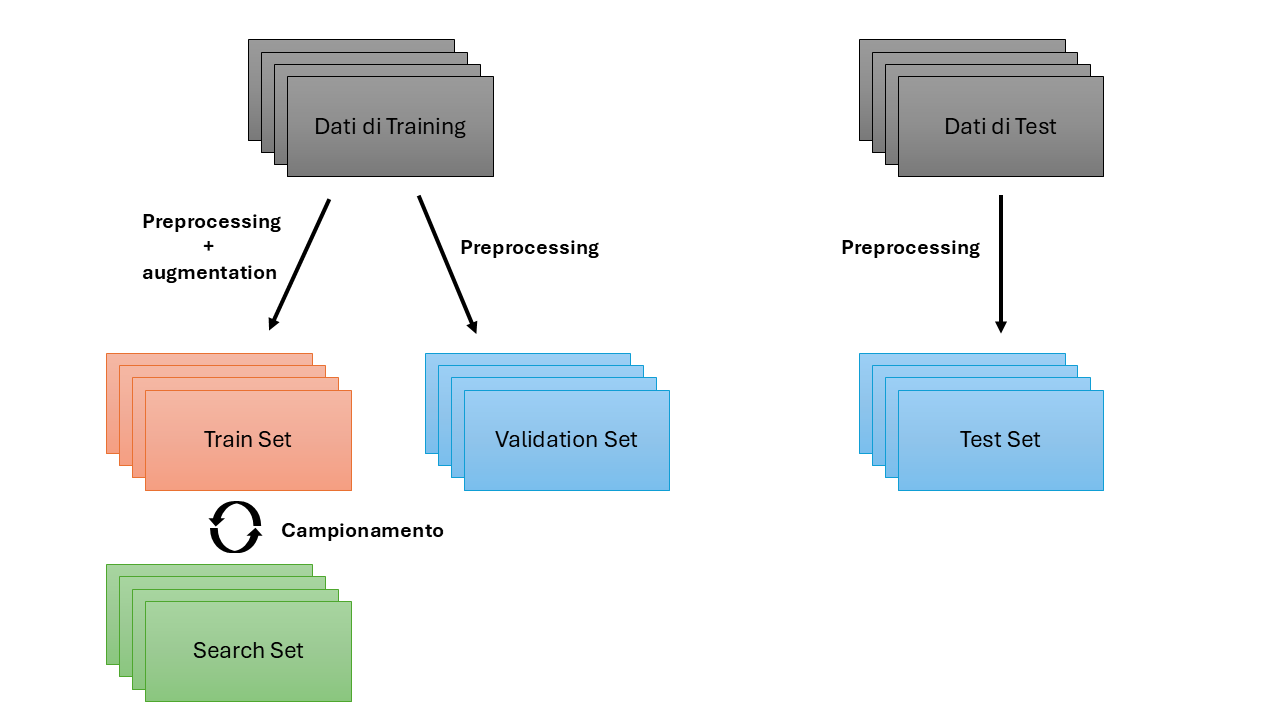
\includegraphics[width=0.7\textwidth]{images/split_dataset.png}
    \caption{Processo di suddivisione del dataset adottato.}
\end{figure}
Per evitare che la fase di ricerca, utilizzando un unico \textit{Search Set} per tutte le iterazioni, provochi un \textit{\textbf{Overfitting Architetturale}}, con conseguenti difficoltà di generalizzazione del modello compresso, il \textit{Search Set} viene \textbf{campionato ad ogni iterazione} a partire dal \textit{Training Set}, fornendo campioni differenti all'algoritmo, di iterazione in iterazione. Questo permette di ottenere un modello risultante che è in grado di generalizzare al meglio sul problema di classificazione, proprio perché l'architettura finale, è il risultato ottenuto con una maggiore quantità e varietà di dati. \par
Un altro contributo fondamentale al mantenimento della capacità di generalizzazione del modello, è dato dalla \textbf{Data Augmentation}, che viene sempre applicata al \textit{Search Set}, ed è la stessa che viene applicata ai dati del \textit{Training Set}. Si potrebbe pensare che questo introduca rumore nei gradienti, e quindi influenzi la precisione e l'affidabilità della metrica di importanza. Nella pratica però il problema del rumore è fortemente limitato dall'utilizzo della media dei gradienti sui batch, per il calcolo della metrica di importanza, com'è possibile osservare nella Formula~\eqref{eq:metrica_importanza}. La \textit{Data Augmentation} applicata al \textit{Search Set} è risultata molto efficace, nei test effettuati, per impedire che venissero sacrificate delle dimensioni del modello essenziali per mantenere la sua capacità di generalizzazione, traducendosi in questo modo in valori di accuratezza sul \textit{Test Set} e sul \textit{Validation Set} più elevati durante tutta l'esecuzione del framework. \par
Notare che è possibile interpretare il framework di compressione come un \textbf{ottimizzazione a due livelli} del modello. In particolare il livello superiore è occupato dal processo di ricerca, che esegue un vero e proprio \textbf{training architetturale}, mentre il livello inferiore è quello del \textit{Fine Tuning}, che invece si occupa di \textbf{ottimizzare i parametri}, date le modifiche architetturali operate dal livello superiore. Questa visione del metodo permette di comprendere al meglio le motivazioni dietro la specifica gestione dei dati, ed in particolare del \textit{Search Set}. Infatti, l'applicazione di tecniche di \textit{data augmentation} a quest'ultimo implica una dinamicità che contribuisce a scongiurare il fenomeno dell'\textit{overfitting architetturale}, analogamente a come tecniche quali l'\textit{early stopping} o i \textit{Learning Rate Scheduler} vengono impiegate per prevenire l'\textit{overfitting} dei parametri del modello.

\section{Framework di Compressione Iterativo}
Una volta definita la strategia di gestione dei dati, è necessario definire la struttura del framework di compressione iterativo, in particolare cosa avviene ad ogni iterazione. \par
\begin{figure}[H]
    \centering
    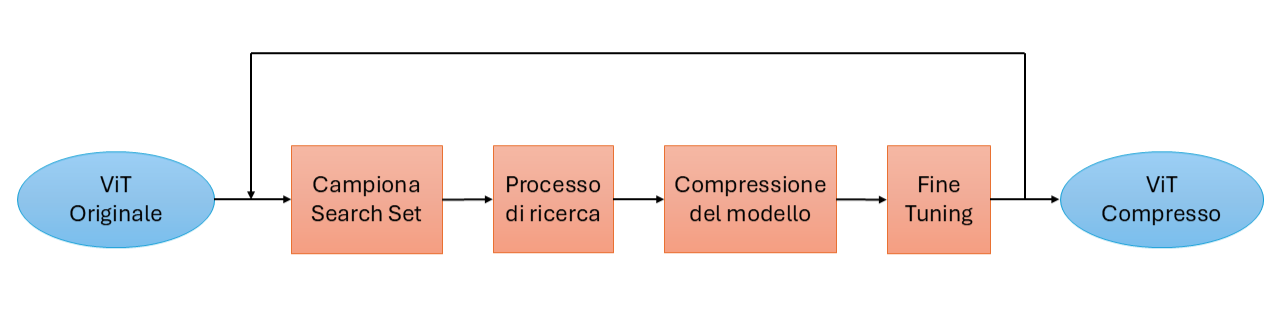
\includegraphics[width=0.9\textwidth]{images/processo.png}
    \caption{Diagramma di flusso del processo di compressione iterativo.}
    \label{fig:processo_compressione}
\end{figure}
Inizialmente viene campionato il \textit{Search Set}, in modo tale da poterlo utilizzare in fase di ricerca. Successivamente inizia la prima fase dell'iterazione: il \textbf{Pruning}. La prima operazione che viene eseguita è l'algoritmo di ricerca \textit{BnB}, che verrà analizzato nella sezione \ref{section:metodo_ricerca}, il quale restituisce lo stato migliore individuato, ovvero una maschera di \textit{pruning} per l'intero modello. \par
A questo punto la maschera viene applicata al modello, e questo viene successivamente ricostruito istanziando tutti i tensori dei parametri ed effettuando una copia solo di quelli non tagliati in fase di ricerca. Viene quindi creato un nuovo modello \textit{ViT}, del quale sono state effettivamente ridotte le dimensioni e questo risulta fondamentale perché implica che il framework proposto non si limita ad applicare delle maschere di \textit{pruning}, che non avrebbero alcun impatto sulle prestazioni effettive del modello sull'hardware, bensì produce dei nuovi modelli di dimensioni realmente minori, con prestazioni realmente superiori. In particolare viene ridotta la latenza in fase di inferenza ma anche la memoria necessaria (VRAM) per utilizzare il modello. \par
Una volta ricostruito il modello, dato che la fase di \textit{Pruning}, avrà introdotto un danno alle performance del modello, è necessario passare alla successiva fase di \textbf{Recovery Fine Tuning}. Si tratta di una serie di epoche di addestramento, volte a consentire ai parametri rimasti del modello di riadattarsi, per poter recuperare l'accuratezza perduta. Risulta fondamentale in questa fase la possibilità di introdurre la \textit{Knowledge Distillation} tramite il modello originale non compresso, che permette tipicamente un recupero più efficace della performance del modello. \par
\begin{algorithm}[H]
\caption{Framework di Compressione Iterativo}
\label{alg:framework_completo}
\begin{algorithmic}[1]
    \State \textbf{Input:} Pre-trained model $M_0$, Dataset $\mathcal{D}$, Iterations $N$, Fine Tuning epochs $K$
    \State \textbf{Output:} Compressed and optimized model $M$
    \State $M_{teacher} \gets M_0$ \Comment{Original model used for distillation}
    \State $M \gets M_0$
    
    \For{$n \gets 1$ \textbf{to} $N$}
        \State $\mathcal{D}_{search} \gets \text{sample\_search\_set}(\mathcal{D}_{train})$ \Comment{Dynamic sampling of the search set}
        \State $m_{pruning} \gets \text{pruning\_algorithm}(M, \mathcal{D}_{search})$ \Comment{obtain pruning mask}
        \State $M_{pruned} \gets \text{compress\_ViT}(M, m_{pruning})$ \Comment{Rebuilding ViT}
        \State $M \gets M_{pruned}$ 
        \State $M \gets \text{FineTuning}(M, M_{teacher}, \mathcal{D}_{train}, \mathcal{D}_{val}, K)$
    \EndFor
    
    \State \Return $M$
\end{algorithmic}
\end{algorithm}

\section{Implementazione dell'algoritmo di ricerca}
\label{section:metodo_ricerca}
In questa sezione viene dettagliata l'implementazione della fase di ricerca con algoritmo \textit{Branch and Bound}, che viene eseguito all'inizio di ogni iterazione di compressione. \par
Al fine di evitare una eccessivo utilizzo di memoria, il processo di ricerca fa utilizzo di stati costituiti come strutture dati a dizionario, invece che vere e proprie copie del modello originale. All'interno di ogni stato è presente una struttura che, per ogni blocco \textit{Transformer} contiene tutte le dimensioni rimosse per ogni tipologia di struttura (MLP, QK, ecc\dots), oltre ad una informazione generale su quali dimensioni di \textit{Embedding} sono state tagliate globalmente. \par
A partire da questa struttura dati è possibile agire su una serie di maschere di \textit{pruning} che vengono applicate al modello, permettendo così di ottenere la vera e propria \textit{subnet}. Per garantire la massima efficienza queste maschere vengono applicate ad un'unica copia del modello iniziale, che, alla fine di ogni esplorazione dello stato vede le proprie maschere reimpostate, per poter applicare i tagli previsti dal successivo stato della ricerca.
\begin{algorithm}[H]
\caption{Ricerca via Depth-First Branch and Bound a profondità limitata}
\label{alg:nas_search}
\begin{algorithmic}[1]
    \State \textbf{Input:} Base Model $M$, Depth Limit $D_{max}$
    \State \textbf{Output:} Optimal State $s_{best}$, Optimal State value $v_{best}$
    \State $s_{init} \gets \text{build\_initial\_state}()$
    \State $stack \gets [s_{init}]$ \Comment{Stack setup}
    \State $M_{work} \gets \text{copy}(M)$
    \State $s_{best} \gets s_{init}$
    \State $v_{best} \gets -\infty$
    \While{$stack$ is not empty}
        \State $s_{curr} \gets stack.\text{pop}()$
        \State $\text{reset\_masks}(M_{work})$
        \State $\text{apply\_masks}(M_{work}, s_{curr})$
        \State $accuracy, active\_params \gets \text{evaluate}(M_{work})$ \Comment{Subnet evaluation}
        \State $v_{curr} \gets \text{compute\_obj}(acc, active\_params)$

        \If{$v_{curr} > v_{best}$}
            \State $v_{best}, s_{best} \gets v_{curr}, s_{curr}$
        \EndIf
        \If{$D_{max}$ reached \textbf{OR} $\text{Bound}(v_{curr}, v_{best})$}
            \State \textbf{continue} \Comment{Bound or depth limit reached}
        \EndIf
        \State // \textit{Branching}
        \State $next\_states \gets \text{Branch}(s_{curr}, M_{work})$
        \For{$s$ in $next\_states$}
            \State $stack.\text{push}(s)$
        \EndFor
    \EndWhile
    
    \State \Return $s_{best}, v_{best}$
\end{algorithmic}
\end{algorithm}




\section{Implementazione delle azioni di Pruning}
\label{section:action_impl}
Data la formulazione matematica delle azioni di ricerca, presentata nella sezione \ref{section:math_actions}, in fase di implementazione, considerato l'elevatissimo numero di dimensioni nel modello, viene addottato un approccio più efficiente.
In particolare, non vengono considerate realmente tutte le possibili combinazioni di dimensioni a $K$ a $K$ di un componente del modello, poiché, dato che è di interesse la somma delle importanze delle singole dimensioni, è sufficiente considerare le $K$ dimensioni le cui importanze sono minime. In particolare, per tutte quelle azioni che agiscono all'interno di un singolo blocco (ovvero tutte tranne il \textit{Pruning} della dimensione di \textit{Embedding}), vengono identificate, per ogni blocco \textit{Transformer} le $K$ dimensioni con il minor valore di importanza. Successivamente, viene selezionato il blocco, il cui gruppo di dimensioni ottimali, hanno una importanza complessiva minore. Questo tipo di approccio semplifica e rende la risoluzione del problema più efficiente. \par
Per quanto riguarda il \textit{Pruning} della dimensione di \textit{Embedding}, l'approccio adottato è il medesimo, con la differenza che, essendo questa una dimensione globale, non vengono considerati singolarmente i blocchi ma complessivamente, riducendo l'algoritmo all'individuazione dei $K$ minimi valori di importanza sull'intero modello. \par
\begin{algorithm}[H]
\caption{Selezione del gruppo di dimensioni ottimale per il taglio}
\label{alg:find_target_gen}
\begin{algorithmic}[1]
    \State \textbf{Input:} Model $M$, Chunk size $K$, Target component $T$
    \State \textbf{Output:} $(\text{block}, [\text{dimension indices}])$ Target dimension group
    \State $v_{best\_imp} \gets \infty$
    \State $target \gets \text{null}$
    
    \For{every block $b$ in $M.blocks$}
        \If{number of dimensions in $T(b) < K$}
            \State \textbf{continue}
        \EndIf
        
        \State $candidates \gets \emptyset$
        
        \For{every dimension $d$ in $T(b)$}
            \If{$d$ is already pruned}
                \State \textbf{continue}
            \EndIf
            \State $imp_d \gets \text{importance\_score}(d)$
            \State $candidates.\text{append}((d, imp_d))$
        \EndFor
        
        \State $candidates \gets$ sort($candidates$, ascending = True) 
        \State $chunk \gets candidates[0 : K]$
        \State $v_{block\_imp} \gets \sum_{(d, i) \in chunk} i$
        
        \If{$v_{block\_imp} < v_{best\_imp}$}
            \State $v_{best\_imp} \gets v_{local\_imp}$
            \State $target \gets (b, \text{chunk.indices})$
        \EndIf
    \EndFor
    
    \State \Return $target$
\end{algorithmic}
\end{algorithm}

\chapter{Esperimenti e risultati}
\label{chap:esperimenti}
In questo capitolo vengono presentati i risultati ottenuti dal framework realizzato, tramite una serie di esperimenti che coinvolgono modelli e dataset differenti.\newline
Tutti gli esperimenti vengono svolti con modelli \textbf{ViT}, preaddestrati sul dataset \textbf{ImageNet}, che lavorano con \textit{patch} di dimensione \textbf{16$\times$16} e immagini in \textit{input} di tipo \textbf{RGB} con risoluzione \textbf{224$\times$224}.

\section{Dataset utilizzati}
Di seguito vengono presentati i dataset utilizzati nei test effettuati sul
framework.

\subsection{CIFAR-100}
Il primo dataset utilizzato per testare il framework è stato il
\textbf{CIFAR100}, che è stato selezionato poiché molto diffuso in letteratura,
in cui è utilizzato come \textbf{benchmark standard} per compiti di
classificazione. Risulta più complesso rispetto al \textit{CIFAR10}, ma
mantiene dimensioni ridotte e quindi permette una ottima rapidità di
\textit{training}. In particolare \textit{CIFAR100} contiene \textbf{60.000
    immagini} totali, suddivise in \textbf{50.000} immagini di addestramento e
\textbf{10.000} di validazione, tutte della risoluzione di
\textbf{32$\times$32} e di tipo \textbf{RGB}. \newline Per i test sul dataset
\textit{CIFAR100} è stata effettuata una ulteriore suddivisione del
\textit{set} di addestramento con rapporto \textbf{90/10}, in modo tale da
ottenere un \textbf{Train Set} finale di \textbf{45.000} immagini e un
\textbf{Held-Out Set} di \textbf{5.000} immagini, quest'ultimo utilizzato per
il monitoraggio del processo di compressione. \newline
\begin{figure}[H]
    \centering
    \includegraphics[width=0.8\textwidth]{images/cifar100_examples.png}
    \caption{Esempio di immagini dal dataset CIFAR100.}
    \label{fig:cifar100_examples}
\end{figure}

\subsection{ImageNet-1K}
Il secondo dataset preso in considerazione per testare il metodo è \textbf{ImageNet-1K}, utilizzatissimo in letteratura e molto più complesso rispetto al CIFAR-100. Si tratta di un \textit{benchmark} utilizzato fin dalle prime reti convoluzionali, come \textit{Alex-Net}, per valutare su task di \textit{Image Classification} e \textit{Object Detection}. Il dataset in questione risulta molto più ampio rispetto al precedente, poiché contiene circa 1.300.000 immagini di addestramento, e 50.000 immagini di validazione, tutte di tipo \textbf{RGB} ma con risoluzione variabile. \newline
Per quanto concerne i test su \textit{Imagenet-1K}, il set di addestramento è stato suddiviso con rapporto \textbf{97/3} al fine di ottenere un \textbf{Held-Out Set} di circa 38.000 immagini, per la validazione del processo di compressione ed eventuale \textit{Early Stop}. 
\begin{figure}[H]
    \centering
    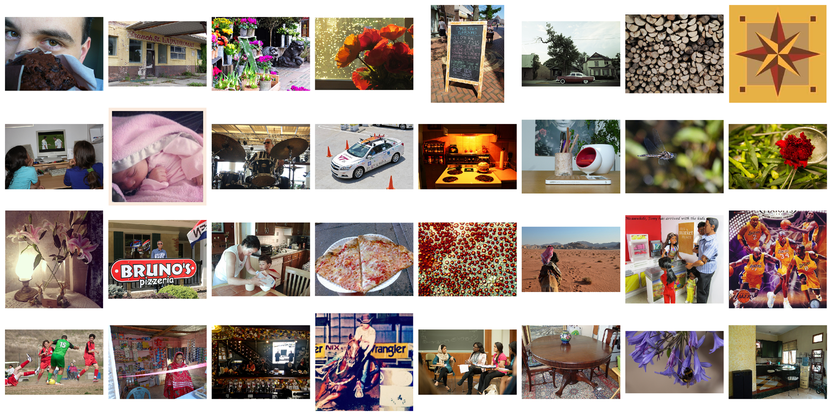
\includegraphics[width=0.9\textwidth]{images/imagenet_examples.png}
    \caption{Esempio di immagini del dataset ImageNet-1K.}
\end{figure}
\section{Data Augmentation}
Data la la grande capacità dei modelli \textit{Vision Transformer}, per
scongiurare il rischio di \textit{overfitting}, sono state adottate delle
tecniche di \textbf{Data Augmentation}, in particolare:
\begin{itemize}
    \item \textbf{Random Resized Crop}: Questa tecnica estrae una porzione casuale dell'immagine originale con un'area compresa tra l'\textbf{80\%} e il \textbf{100\%} della dimensione iniziale. Successivamente, il ritaglio viene ridimensionato alla risoluzione \textit{target} di \textbf{$224 \times 224$} pixel.
    \item \textbf{Random Horizontal Flip}: Consiste nel riflettere l'immagine orizzontalmente con una probabilità del \textbf{50\%}.
    \item \textbf{Color Jitter}: Questa trasformazione applica variazioni casuali alla luminosità, al contrasto e alla saturazione dell'immagine, con un fattore di distorsione impostato a \textbf{0.3} per ciascun parametro.
\end{itemize}
Queste sono state utilizzate per il dataset CIFAR100.

\section{Dettaglio implementativo}
\label{section:impl}
Di seguito i dettagli implementativi delle fasi di \textit{Fine Tuning} dei
modelli, durante la compressione. Per il primo \textit{Fine Tuning}:
\begin{itemize}
    \item \textbf{Ottimizzatore AdamW} con un fattore di \textbf{decadimento dei pesi} pari a \textbf{0.05} e con \textbf{learning rate discriminativi}: \textbf{$0.5 \times 10^{-5}$} per il \textit{backbone} del \textit{Transformer} e \textbf{$0.5 \times 10^{-4}$} per la testa di classificazione.
    \item \textbf{Scheduler} dei \textit{learning rate} di tipo \textbf{Cosine Annealing}.
    \item Dimensione dei \textbf{batch} di \textit{training} pari a \textbf{128}
          campioni.
    \item \textbf{30 epoche} di addestramento con \textbf{early stopping}.
\end{itemize}
Per quanto riguarda invece la fase di \textbf{Recovery Fine-Tuning}, volta a
ripristinare le prestazioni dopo il taglio dei parametri, adotta la medesima
configurazione di ottimizzazione del \textit{Fine-Tuning} iniziale, con due
variazioni: l'impiego di un \textbf{learning rate unico} pari a \textbf{$0.5
        \times 10^{-5}$} per l'intera rete e un limite massimo di \textbf{20 epoche} di
addestramento, sufficienti per stabilizzare i pesi della \textit{subnet}
individuata. \newline Infine, per quanto concerne i test con la
\textbf{Knowledge Distillation} (\textbf{KD}), è stata implementata una
versione \textit{logit-based} seguendo l'approccio proposto da \textit{Hinton
    et al.} \cite{hinton2015distilling}. Il modello \textbf{teacher}, in tutti i test, consiste nel modello \textit{ViT} che fa da \textit{Baseline}, ovvero quello integro, non sottoposto ad alcuna compressione. La funzione di
\textbf{loss composita} utilizzata durante il \textit{Recovery Fine-Tuning}
integra un termine di distillazione con temperatura \textbf{$\tau = 4.0$}. A
tale componente è stato assegnato un \textbf{peso relativo pari a $0.9$},
privilegiando così il trasferimento della conoscenza dal modello
\textit{teacher} alla \textit{subnet} compressa. Questa configurazione ha
permesso di ammorbidire le distribuzioni di probabilità dei \textit{logits},
consentendo al modello \textit{student} di apprendere non solo le etichette
corrette, ma anche le relazioni strutturali tra le classi catturate dal modello
completo. Di seguito i risultati dei test. \newline

\section{Metriche}
Per valutare le prestazioni dei modelli nei test effettuati, e di conseguenza per valutare l'efficacia del framework di compressione, sono state utilizzate le seguenti metriche:
\begin{itemize}
    \item \textbf{Numero di Parametri}: consiste nella quantità di parametri rimasti al modello, dopo l'esecuzione del processo di compressione.
    \item \textbf{Accuracy}: al fine di valutare le prestazioni del modello sul task di riferimento, viene utilizzata la \textit{Top-1 Accuracy}, valutata sui dati di test del dataset utilizzato.
    \item \textbf{GFLOPs}: si tratta del numero di \textit{Floating Point Operations} (operazioni in virgola mobile) che sono necessarie per eseguire un singolo passaggio di inferenza (\textit{forward pass}) sul modello. In particolare 1 GFLOP corrisponde ad $1 \times 10^9$ operazioni in virgola mobile. A differenza della latenza, che risulta legata all'hardware utilizzato, i GFLOPs forniscono una misura deterministica della complessità computazionale del modello.
    \item \textbf{Throughput}: consiste nel numero di immagini al secondo che vengono processate dal modello, e viene calcolato costruendo un batch di immagini "fittizie", ovvero ottenute tramite la generazione di un tensore randomico, e successivamente misurando il tempo necessario al modello per eseguire l'inferenza su tale tensore.
    \item \textbf{Latency}: viene calcolata insieme alla precedente, e misura (in ms) il tempo necessario per l'inferenza di un singolo batch di immagini.  
\end{itemize}


\section{Test sul dataset CIFAR-100}
\label{section:test}
\subsection{Test con ViT-Small}
In questi test è stato utilizzato un modello \textbf{ViT-Small} da \textbf{21.7
    Mln} di parametri, a cui è stata aggiunta una testa di classificazione da
\textbf{100 unità}, e successivamente sottoposto a \textit{Fine Tuning}
iniziale sul dataset in oggetto. Per quanto riguarda il framework, tutti i test
sono stati effettuati con \textbf{15 iterazioni} di compressione. In ogni
iterazione, la \textbf{profondità} dell'albero di ricerca è stata limitata a
\textbf{6}, questo implica che, per ogni iterazione, al modello possono essere
applicate massimo \textbf{6 azioni consecutive} di \textit{pruning}. Viene
inoltre utilizzata una \textbf{soglia di tolleranza} della fase di
\textit{Bound} pari a \textbf{0.005}, in modo tale da permettere una ricerca
più approfondita dello spazio di ricerca, al costo di un numero lievemente
maggiore di nodi esplorati. Infine, la \textbf{funzione obiettivo} utilizza un
valore di \textbf{$\lambda$} pari a \textbf{1.0}, attribuito al contributo dei
parametri. \newline 
\begin{table}[ht]
    \centering
    \label{tab:risultati-cifar100}
    \footnotesize 
    \setlength{\tabcolsep}{3pt} 
    \begin{tabular}{@{} l r r r r r @{}}
        \toprule
        \textbf{Modello} & \multicolumn{1}{c}{\textbf{Parametri (M)}} & \multicolumn{1}{c}{\textbf{Top-1 Acc. (\%)}} & \multicolumn{1}{c}{\textbf{GFLOPs}} & \multicolumn{1}{c}{\textbf{Throughput}} & \multicolumn{1}{c}{\textbf{Latency}} \\ \midrule
        Baseline           & 21.67 \hphantom{(-00.0\%)}        & 90.42\% \hphantom{(-0.00\%)}        & 4.60 \hphantom{(-00.00\%)}        & 1137.5 \hphantom{(+00.00\%)}        & 112.5 \hphantom{(-00.00\%)}       \\
        \midrule
        \textbf{Pruned}    & 15.93 (-26.6\%) & 89.59\% (-0.83\%) & 3.42 (-25.51\%) & 1405.5 (+23.56\%) & 91.1 (-19.02\%) \\
        \midrule
        \textbf{Pruned+KD} & 15.78 (-27.3\%) & 89.86\% (-0.56\%) & 3.39 (-26.19\%) & 1406.0 (+23.60\%) & 91.0 (-19.11\%) \\
        \bottomrule
    \end{tabular}
    \vspace{10pt}
    \caption{Nella tabella sono presentati i risultati comparativi utilizzando il \textit{ViT-Small} e il dataset \textit{CIFAR100}, in particolare vengono evidenziati i valori delle metriche e le variazioni rispetto al modello \textit{Baseline}.}
\end{table}

\section{Test sul dataset ImageNet-1K}
Per questi test è stato utilizzato un modello \textbf{ViT-Small} da 22 Mln di parametri. In particolare è stata aggiunta una testa di classificazione da 1000 unità, che è stata sottoposta a \textit{fine tuning} sul \textit{train set} con la \textit{backbone} del modello \textit{ViT-Small} bloccata. I parametri del framework, per tutti i test, sono stati configurati a \textbf{15 iterazioni} di compressione, la \textbf{profondità} dell'albero di ricerca è stata limitata a
\textbf{6}, la \textbf{soglia di tolleranza} della fase di
\textit{Bound} pari a \textbf{0.005}, la \textbf{funzione obiettivo} con \textbf{$\lambda$} pari a \textbf{1.0} per i parametri. \newline 
\begin{table}[ht]
    \centering
    \label{tab:risultati-cifar100}
    \footnotesize 
    \setlength{\tabcolsep}{3pt} 
    \begin{tabular}{@{} l r r r r r @{}}
        \toprule
        \textbf{Modello} & \multicolumn{1}{c}{\textbf{Parametri (M)}} & \multicolumn{1}{c}{\textbf{Top-1 Acc. (\%)}} & \multicolumn{1}{c}{\textbf{GFLOPs}} & \multicolumn{1}{c}{\textbf{Throughput}} & \multicolumn{1}{c}{\textbf{Latency}} \\ \midrule
        Baseline           & 22.05 \hphantom{(-00.0\%)}        & 81.20\% \hphantom{(-0.00\%)}        & 4.60 \hphantom{(-00.00\%)}        & 1142.6 \hphantom{(+00.00\%)}        & 112.0 \hphantom{(-00.00\%)}       \\
        \midrule
        \textbf{Pruned}    & 18.77 (-14.88\%) & 79.17\% (-2.03\%) & 3.90 (-15.13\%) & 1270.5 (+11.20\%) & 100.7 (-10.07\%) \\
        \bottomrule
    \end{tabular}
    \vspace{10pt}
    \caption{Nella tabella sono presentati i risultati comparativi utilizzando il \textit{ViT-Small} e il dataset \textit{ImageNet-1K}, in particolare vengono evidenziati i valori delle metriche e le variazioni rispetto al modello \textit{Baseline}.}
\end{table}

\section{Analisi dell'algoritmo di ricerca}
Fare test con la loss nella funzione obbiettivo, poi un altro senza la soglia
nel bound e con vari valori.

\section{Ablazione}
Al fine di verificare la bontà del metodo sono stati effettuati dei test per isolare il contributo delle due principali componenti del \textit{framework}, l'algoritmo di ricerca e la metrica di importanza. \newline
I seguenti risultati sono stati ottenuti sul dataset CIFAR100, utilizzando la stessa configurazione riportata nella sezione \ref{section:test} e nella sezione \ref{section:impl}. I test sono stati eseguiti senza l'utilizzo della \textit{Knowledge Distillation} per isolare al meglio l'effetto delle singole componenti del framework. \newline
Di seguito i risultati: \newline 
\begin{table}[ht]
    \centering
    \label{tab:risultati-ablazione}
    \footnotesize 
    \setlength{\tabcolsep}{3pt} 
    \begin{tabular}{@{} l r r r r r @{}}
        \toprule
        \textbf{Modello} & \multicolumn{1}{c}{\textbf{Parametri (M)}} & \multicolumn{1}{c}{\textbf{Top-1 Acc. (\%)}} & \multicolumn{1}{c}{\textbf{GFLOPs}} & \multicolumn{1}{c}{\textbf{Throughput}} & \multicolumn{1}{c}{\textbf{Latency}} \\ \midrule
        Baseline           & 21.67 \hphantom{(-00.0\%)}        & 90.42\% \hphantom{(-0.00\%)}        & 4.60 \hphantom{(-00.00\%)}        & 1137.5 \hphantom{(+00.00\%)}        & 112.5 \hphantom{(-00.00\%)}       \\
        \midrule
        \textbf{ViT-S Pruned (No KD)}    & 15.93 (-26.6\%) & 89.59\% (-0.83\%) & 3.43 (-25.51\%) & 1405.5 (+23.56\%) & 91.1 (-19.02\%) \\
        \midrule
        \textbf{Ricerca Disattivata} & 12.28 (-43.4\%) & 81.17\% (-9.25\%) & 2.64 (-42.66\%) & 1679.9 (+47.68\%) & 76.2 (-32.27\%) \\
        \midrule
        \textbf{Metrica Disattivata} & 19.38 (-10.7\%) & 89.07\% (-1.35\%) & 4.09 (-11.09\%) & 1147.9 (+00.09\%) & 111.5 (-00.09\%) \\
        \bottomrule
    \end{tabular}
    \vspace{10pt}
    \caption{Nella tabella sono presentati i risultati dell'applicazione del \textit{framework} di compressione nella sua interezza e con le componenti disattivate, sul dataset \textit{CIFAR100} e sul modello \textit{ViT-Small}.}
\end{table}

Come è possibile notare, entrambi i test di ablazione hanno dato risultati peggiori rispetto a quanto ottenuto con il \textit{framework} di compressione nella sua interezza. In particolare nel test con la \textbf{ricerca disattivata}, per ogni iterazione, considerando $d$ la massima profondità della ricerca, vengono eseguite casualmente $d$ azioni sul modello. In questo caso il \textit{framework} si è trovato costretto ad eseguire dei tagli su dimensioni importanti, e quindi poco conservativi dal punto di vista delle performance. La metrica di importanza, mantenuta attiva nel test, non è riuscita a limitare i danni portati dai tagli molto aggressivi e indiscriminati, portando così ad una grande diminuzione di accuratezza. Questo primo test ha dimostrato che l'algoritmo di ricerca \textit{BnB} ha un grande contributo nel selezionare accuratamente le azioni, da un lato limitando il livello di compressione a parità di iterazioni di \textit{pruning}, dall'altro consentendo di mantenere dei livelli di prestazioni molto vicini al modello originale. \newline 
Nel secondo test invece, la \textbf{metrica di importanza} è stata disattivata, di conseguenza per ogni azione selezionata dall'algoritmo di ricerca, viene prima selezionato casualmente il blocco \textit{Encoder} su cui agire, e successivamente vengono campionate casualmente le dimensioni da tagliare delle specifiche componenti (QK, MLP, \dots) di quel blocco (tranne per la dimensione di \textit{Embedding}, per il quale non è necessario selezionare prima il blocco su cui agire). I risultati indicano chiaramente una difficoltà dell'algoritmo di ricerca nell'esplorare lo spazio degli stati, causata proprio dalla mancanza dell'azione della metrica di importanza. Selezionando in maniera casuale le dimensioni da tagliare, la maggioranza degli stati (\textit{subnet}) che vengono esplorati risultano poco promettenti e peggiorano il valore della funzione obbiettivo, con un conseguente aumento del numero di nodi esplorati, ed una grande fatica a comprimere il modello. Durante i test che fanno uso della metrica di importanza, si assiste invece ad una progressione stabile e rapida del valore della funzione obbiettivo, che si dimostra quindi molto efficace nel guidare le azioni di \textit{pruning} e la ricerca. \newline 
In questo secondo test è importante notare come le prestazioni del modello si sono mantenute elevate, a conferma del grande lavoro di filtraggio eseguito dal processo di ricerca, che evita di selezionare quegli stati, la cui selezione casuale dei tagli, ha danneggiato gravemente il modello. 



\include{capitoli/ch5}
% ...



%% Conclusioni
\clearpage
\phantomsection
\addcontentsline{toc}{chapter}{Conclusioni}
\chapter*{Conclusioni}
\markboth{Conclusioni}{}

In questo lavoro è stato progettato, implementato e validato un framework automatico per la compressione e l'ottimizzazione di modelli \textit{Vision Transformer} (ViT), con l'obiettivo di ridurne l'impatto computazionale e renderne possibile l'esecuzione efficiente su architetture hardware a risorse limitate, come i dispositivi mobili ed \textit{edge}. La strategia proposta ha integrato una tecnica di \textit{pruning} strutturato con gli algoritmi di ottimizzazione, unendo anche la \textit{Knowledge Distillation}. \par

L'analisi sperimentale, condotta su benchmark standard quali \textit{CIFAR-100} e \textit{ImageNet-1K}, ha confermato l'efficacia dell'approccio e la sua competitività con lo stato dell'arte. I risultati quantitativi hanno evidenziato che sia possibile ottenere una riduzione di circa un terzo dei parametri e dei GFLOPs, con una perdita di accuratezza trascurabile, che corrisponde però ad un incremento significativo del throughput. Sono stati inoltre condotti dei test di inferenza su dispositivi mobili, dimostrando l'impatto reale della compressione sulle latenze registrato a seguito della procedura di \textit{deploy}. \par

Gli studi di ablazione hanno validato l'architettura interna del framework, dimostrando che sia la metrica di importanza basata sul Fisher Score, sia la componente di ricerca contribuiscono ad evitare il decadimento delle prestazioni durante il processo di compressione. \par

Nell'analisi dei risultati ottenuti dai test sono emersi alcuni pattern strutturali interessanti che portano ad alcune considerazioni sulla natura dei modelli ViT e sul loro funzionamento. Da quanto osservato emerge una struttura ad "U", già teorizzata e studiata nella letteratura recente, secondo il quale i layer centrali contengono le rappresentazioni ad alto livello, i concetti semantici, e di conseguenza sono più sensibili al pruning. 


\section{Limitazioni e sviluppi futuri}
Di seguito sono elencate alcune limitazioni del lavoro svolto e possibili sviluppi futuri che potrebbero essere intrapresi per migliorare ulteriormente il framework di compressione proposto:

\begin{itemize}
    \item \textbf{Costo computazionale della compressione:} Il framework di compressione presentato, nonostante l'efficacia dimostrata, richiede un costo computazionale considerevole. Se in particolare si vuole recuperare la massima \textit{accuracy} possibile, è necessario utilizzare un numero elevato di epoche di \textit{fine tuning}, che, se unito ad un elevato numero di iterazioni di ricerca, può portare a costi paragonabili a quelli di un addestramento completo del modello originale. Nonostante ciò, è importante sottolineare che il processo di compressione rappresenta un investimento da eseguire in una singola occasione, che presenta benefici tangibili che potrebbero comunque risultare vantaggiosi in scenari di produzione.
    
    \item \textbf{Mancanza di test sui modelli di grandi dimensioni:} A causa dell'elevato costo computazionale prima esposto, i test sperimentali sono stati condotti su modelli di dimensioni ridotte, che rappresentano comunque un'ottima sfida per la compressione, tuttavia non è stato possibile estendere l'analisi a modelli di maggiori dimensioni, che potrebbero beneficiare maggiormente di un processo di questo tipo. Sarebbe inoltre auspicabile estendere l'analisi a modelli di maggiori dimensioni al fine di verificare la presenza degli stessi pattern strutturali osservati nel test condotti in questo lavoro, in maniera tale da confermare ulteriormente le considerazioni formulate attraverso l'analisi dei risultati.

    \item \textbf{Estensione a compiti di visione complessi:} Oltre a testare il framework su modelli di maggiori dimensioni, sarebbe utile eseguire dei test al di fuori del \textit{task} di classificazione. Questo consentirebbe di verificare la bontà del processo su modelli utilizzati come \textit{backbone} per compiti di \textit{object detection}, \textit{semantic segmentation} o modelli multimodali.
    
    \item \textbf{Confronto con metodo Greedy:} Dato l'impiego di un algoritmo di ricerca avanzato per l'individuazione delle migliori azioni di \textit{pruning} da attuare, sarebbe necessario un confronto con un implementazione di tipo \textit{greedy} del metodo. Tale comparazione permetterebbe di verificare una eventuale superiorità del processo di ricerca con algoritmo \textit{Branch and Bound} rispetto a quanto proposto in questo lavoro, giustificando così l'incremento del costo computazionale.

    \item \textbf{Integrazione con tecniche di quantizzazione:} Il beneficio computazionale potrebbe essere ulteriormente amplificato combinando il \textit{pruning} strutturato con tecniche di quantizzazione post-addestramento (PTQ) o quantizzazione di tipo \textit{training-aware}(QAT). L'integrazione di queste tecniche, oggi molto diffuse nell'ambito dei \textit{Large Language Models} (LLM) e pienamente supportate dall'hardware, permetterebbero di ottenere modelli ancora più performanti, al costo di un leggero decadimento delle prestazioni predittive.
    
    \item \textbf{Applicazione a modelli di tipo \textit{Large Language Models} (LLM):} Un interessante sviluppo futuro potrebbe essere rappresentato dall'estensione del framework a modelli di tipo LLM, che presentano un numero di parametri estremamente elevato, e che potrebbero beneficiare in maniera significativa da un processo di compressione. L'applicazione del framework a questo tipo di modelli potrebbe richiedere alcune modifiche alla strategia di compressione, ma rappresenterebbe un importante passo avanti. La più grande limitazione in questo caso sarebbe costituita dal costo computazionale, che potrebbe essere proibitivo, tuttavia si potrebbe mitigarlo attraverso l'impiego di tecniche di \textit{parameter efficient fine tuning} (PEFT), che permetterebbero di ridurre significativamente il numero di parametri da aggiornare durante la fase di \textit{fine tuning}.
    
    \item \textbf{Utilizzo di tecniche di Token Pruning:} Un ulteriore direzione di ricerca potrebbe essere rappresentato dall'integrazione di tecniche di \textit{token pruning}, che permetterebbero di ridurre in maniera significativa il costo computazionale durante la fase di inferenza, eliminando i token meno rilevanti per la predizione. Questo è facilmente visibile nei risultati ottenuti in \cite{wang2025caittriplewincompressionhigh}, nel quale è stato adottato sia un processo di \textit{pruning} strutturato, sia una tecnica di \textit{token merging}, ottenendo un incremento del 90\% di \textit{throughput}.
    
\end{itemize}





%% Ringraziamenti
\clearpage
\phantomsection
\addcontentsline{toc}{chapter}{Ringraziamenti}
\chapter*{Ringraziamenti}

Desidero esprimere la mia più profonda gratitudine, in primo luogo, alla mia Relatrice, la \relatore, per avermi guidato con costante disponibilità, pazienza e rigore scientifico lungo tutto lo sviluppo di questo lavoro di ricerca. I suoi preziosi consigli e la fiducia che ha riposto nelle mie intuizioni sono stati fondamentali per il superamento delle sfide incontrate lungo il percorso. \par
Successivamente desidero ringraziare tutti i miei colleghi di laboratorio, in particolare i due Gabriele, che mi hanno fornito tante opportunità di confronto e crescita, e mi hanno tirato su nei momenti in cui il morale poteva vacillare. \par 
Un ringraziamento speciale va poi a Gianvito, con il quale ho condiviso questo percorso di studi, una casa e soprattutto un'amicizia sincera e fraterna. \par
Un grazie di cuore va alla mia famiglia e ai miei amici, che mi hanno sempre sostenuto, incoraggiato ma soprattutto sopportato, in questi anni di stress e sacrifici. Senza di loro, questo traguardo non sarebbe stato possibile. \par
Infine, grazie a Paola per essere stata al mio fianco, per tutto il suo amore, la sua pazienza e il suo supporto incondizionato. Senza di lei, questo percorso sarebbe stato molto più difficile e noioso. La sua presenza e il suo affetto sono stati una fonte inesauribile di forza e motivazione. \par
A tutti voi, il mio più sincero grazie.



%% Indice delle figure
\clearpage
\phantomsection
\addcontentsline{toc}{chapter}{Elenco delle figure}
\listoffigures


%% Bibliografia
\clearpage

\phantomsection
\addcontentsline{toc}{chapter}{\bibname}
\markboth{Bibliografia}{}
\printbibliography[heading=bibliografia]

\end{document}